\chapter{Introducción}

    \section{Motivación}
        
        La Agencia Digital de Andalucía presentó en 2021 un plan de inversión para los años 2022-2025 que se centra en varias áreas estratégicas de desarrollo tecnológico, incluyendo la ciberseguridad. Esta inversión del Gobierno andaluz no solo impulsará la creación de un Centro de Ciberseguridad que coordinará la Estrategia Andaluza de Ciberseguridad, sino que además, pretende conseguir que revierta en el desarrollo económico de la región, que ya ha empezado a aceptar empresas como Google, que ha instalado su Centro de Excelencia de Ciberseguridad en Málaga.
        
        Bajo el paraguas de este desarrollo tecnológico, el aumento de la demanda de profesionales en este campo ha despertado un gran interés en los estudiantes por aprender sobre la ciberseguridad.
        
        Sin embargo, muchos de ellos se enfrentan a la dificultad de encontrar recursos educativos completos y accesibles debido a las restricciones que imponen algunas plataformas de entrenamiento, donde los recursos que ofrecen tienen barreras que dificultan el acceso a la formación, incluyendo la necesidad de suscripciones para acceder al contenido completo.
        
        Esto puede desmotivar a los estudiantes y reducir su capacidad para aprender y desarrollar habilidades en el campo de la ciberseguridad.
    
    
    \section{Objetivos}
        \label{sec:objetivos}
    
        Se busca desarrollar una plataforma web que sea ligera, gratuita, \textit{open-source} y fácilmente extensible, con el objetivo principal de simplificar la introducción de futuros estudiantes en el sector de la ciberseguridad, con un enfoque específico en el pentesting.
        
        La plataforma proporcionará información documentada y sintetizada junto con entornos de prueba virtualizados (laboratorios) para facilitar el aprendizaje mediante la experimentación.
        
        A diferencia de otras plataformas como Hack The Box y similares, el enfoque de esta plataforma no estará en la resolución de retos, como serían las pruebas de tipo CTF más habituales en el sector, sino en guiar e instruir a los usuarios de la plataforma sobre distintos conceptos y técnicas de pentesting, proporcionando entornos virtuales diseñados específicamente para experimentar y poner en práctica conceptos concretos.
        
        Esta herramienta brindará a los usuarios una experiencia educativa gratuita y accesible en ciberseguridad, permitiéndoles aprender y desarrollar habilidades prácticas de manera efectiva y en línea con las necesidades del mercado.
    
    
    \section{Metodología}
    
        Se ha empleado un desarrollo incremental para la elaboración del proyecto: se partió de una base a la que se añadieron sucesivas mejoras sin que estas perjudicaran al resto del proyecto desarrollado hasta ese momento.

        \begin{figure}[htbp]
            \centering

            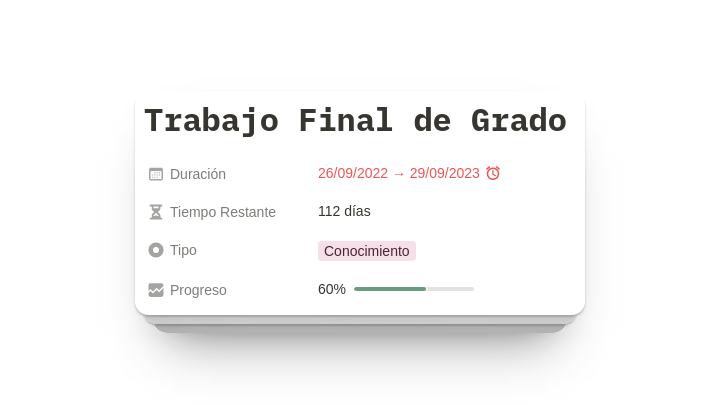
\includegraphics[width=0.75\textwidth]{images/Capturas/Notion resumen.png}

            \caption{Resumen del estado del proyecto en Notion al momento de la captura}
            \label{fig:notion-resumen}
        \end{figure}

        Se ha utilizado la herramienta Notion para llevar a cabo este proyecto, una aplicación que permite la creación de notas -llamadas páginas- cuyo contenido puede ser variado: texto, imágenes, tablas, listas, archivos, enlaces, etc. y que además, permite la creación de bases de datos que pueden ser utilizadas para definir tablones Kanban, diagramas de Gantt, y otros tipos de vistas dinámicas.

        Notion también cuenta con otra funcionalidad recientemente añadida: la integración con GitHub \cite{github}. Esto permite añadir a cualquier página de Notion una base de datos generada a partir del estado de un repositorio remoto -\textit{Issues}, \textit{Projects} y \textit{Pull Requests}-, permitiendo además la manipulación y la actualización del contenido en ambas direcciones, todo sincronizado en tiempo real. 

        El proceso que se ha seguido para el desarrollo del proyecto ha sido definir tareas en Notion y descomponerlas en tareas más simples, atómicas y tratables, clasificadas en función de su propósito: componer la memoria, desarrollar la plataforma web o crear entornos de pruebas virtualizados (sección \ref{sec:estructura-global}). Por otra parte, se han asignado dependencias entre las tareas, por lo que en la mayoría de ocasiones resultaba intuitivo y visual establecer el orden que debían seguir dichas tareas.

        \newpage

        \begin{figure}[!htbp]
            \centering

            \begin{subfigure}[!htbp]{\textwidth}
                \centering

                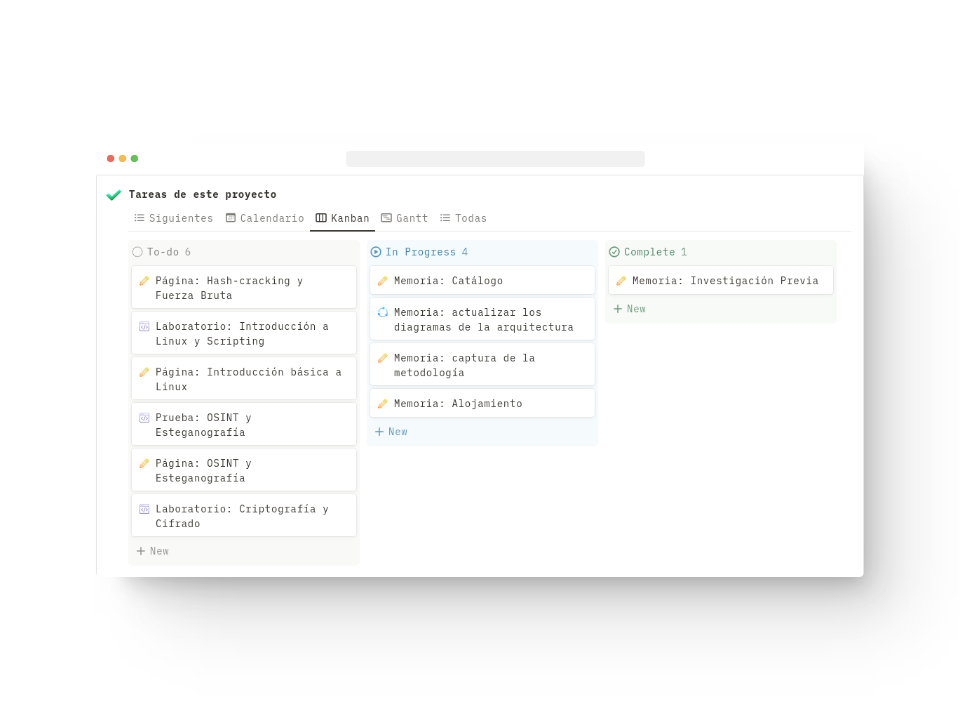
\includegraphics[width=0.8\textwidth]{images/Capturas/Notion Kanban.png}
                \caption{Vista de Kanban}
            \end{subfigure}
            
            \begin{subfigure}[!htbp]{\textwidth}
                \centering

                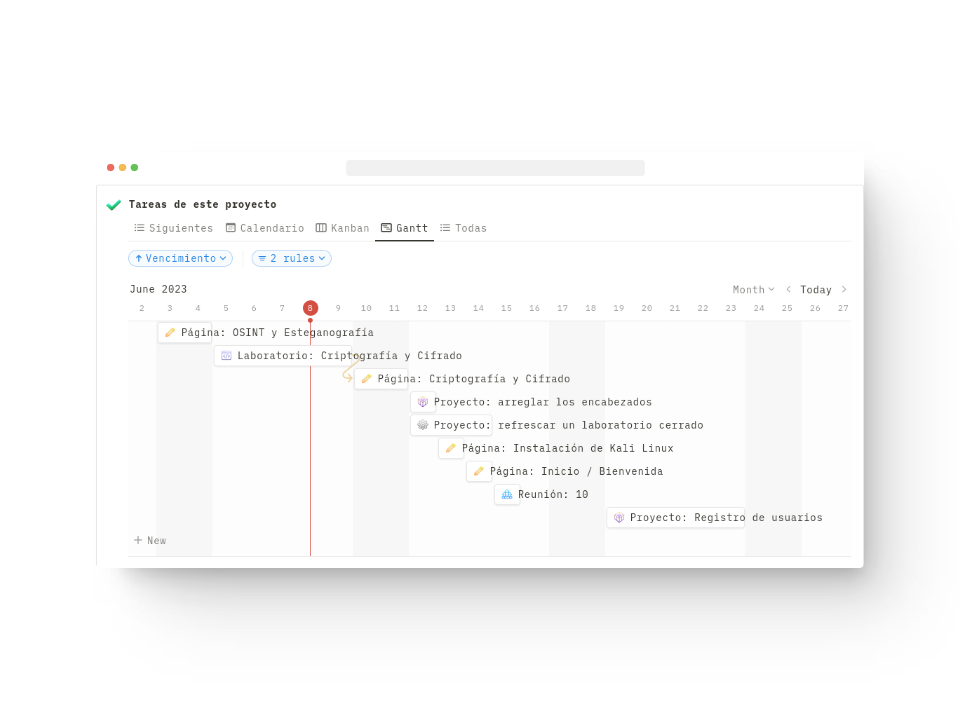
\includegraphics[width=0.8\textwidth]{images/Capturas/Notion Gantt.png}
                \caption{Vista de Gantt}
            \end{subfigure}
            
            \caption{Gestión de tareas del proyecto en una base de datos de Notion}
            \label{fig:notion-vistas}
        \end{figure}
        
        El desarrollo se ha llevado a cabo utilizando, principalmente, las vistas de los sistemas: Kanban, con las tareas clasificadas en función de su estado; y Gantt, con las tareas clasificadas y ordenadas en función de sus dependencias. No obstante, también se han utilizado las vistas de Lista para visualizar las tareas de una forma más compacta y ordenada, y de Calendario para visualizar las tareas en función de su fecha de finalización.
        
        \newpage
    

    \section{Estructura global del proyecto}
        \label{sec:estructura-global}
        
        El proyecto se divide en tres pilares principales: la creación de una plataforma web, la investigación -y selección- de conceptos de pentesting y la virtualización de los entornos de prueba:
        
        \begin{figure}[h]
            \centering

            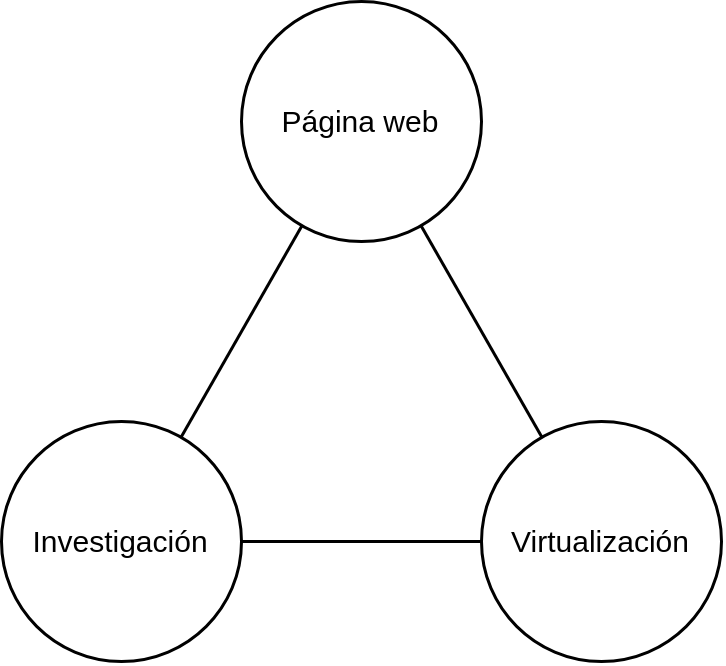
\includegraphics[scale=0.30]{images/Diagramas/Estructura global.png}
            
            \caption{Pilares fundamentales del proyecto}
            \label{fig:estructura-global}
        \end{figure}
            
        \subsection{Página web}
        
            La primera toma de contacto del usuario con la plataforma, la página web será la interfaz de usuario para acceder a los laboratorios y contenidos relacionados con la ciberseguridad.
            
            Respecto a su construcción, se han considerado dos opciones:
            
            \begin{itemize}
                \item \textbf{Programación desde cero}: se consideró el uso del framework Astro, que permite crear sitios web rápidamente, además de proporcionar un amplio conjunto de herramientas para su personalización.
                \item \textbf{Utilizar un CMS (Sistema de Gestión de Contenido)}: se consideró el uso de WordPress, uno de los CMS más utilizados en el mundo y que cuenta con una amplia variedad de plantillas disponibles, lo que facilitaría el diseño de la interfaz.
            \end{itemize}

            Finalmente, se decidió usar WordPress por su sencillez y su biblioteca de plugins, que permitiría integrar diferentes funcionalidades extra en lugar de programarlas manualmente como podría haber ocurrido con el uso de un framework.
                
            \subsubsection{Alojamiento}
            
                Respecto al alojamiento, se han considerado varias opciones, tales como GitHub Pages, Vercel, OVHcloud o Heroku.
                
                Sin embargo, al tratarse de una prueba de concepto, se ha decidido elaborar la infraestructura de forma local, lo que permitirá un mayor control y flexibilidad en el desarrollo, dando lugar a mejoras en futuras líneas de trabajo (sección \ref{sec:futuras-lineas-trabajo}).

                En cuanto a la base de datos, se ha decidido utilizar MySQL por ser una opción muy utilizada, fácil de configurar y ser nativamente compatible con WordPress. La base de datos tendrá la menor cantidad de tablas posibles, almacenando únicamente la información necesaria sobre los usuarios registrados y sobre los laboratorios.
            
        \subsection{Investigación}
        
            Se centrará en recopilar y seleccionar diferentes conceptos y técnicas relacionados con el pentesting. Este apartado se verá mejor reflejado en la sección \ref{cap:catalogo}.

            La investigación se llevará a cabo en paralelo con el desarrollo de la plataforma web, ya que los resultados de la investigación se utilizarán para crear los laboratorios.
        
        \subsection{Virtualización}

            La virtualización es una parte integral del proyecto, ya que permite la creación de varios laboratorios de prueba donde los usuarios aplicarán los conocimientos adquiridos en la plataforma. Concretamente, se consideraron contenedores de Docker y máquinas virtuales para crear estos laboratorios.
            
            Elegir Docker como plataforma de contenedores es una buena opción porque ofrece una gestión de recursos eficiente y una generación de imágenes sencilla; por otro lado, Vagrant Cloud es una buena opción para crear máquinas virtuales, ya que ofrece una amplia gama de imágenes preconfiguradas y un entorno de desarrollo fácil de usar.
            
            Por otro lado, también se consideraron plataformas que brindan servicios de almacenamiento y distribución de imágenes, como DockerHub para imágenes de contenedores de Docker y Vagrant Cloud para máquinas virtuales preconfiguradas. Estas dos plataformas brindan enlaces de descargas con las que un usuario puede acceder a recursos previamente construidos por su autor.

            \newpage

            
    \section{Tecnologías empleadas}
        \label{tecnologias}

        Esta sección recoge de forma directa las tecnologías y herramientas que se usaron para llevar a cabo el proyecto. Algunas de ellas fueron una elección clara, mientras que otras pasaron por un proceso de análisis, recogido en la sección \ref{analisis-tecnologias}.
        
        \subsection{GitHub}
        
            GitHub es una plataforma de desarrollo colaborativo de software que ofrece alojamiento de código fuente, seguimiento de problemas y herramientas de colaboración para proyectos de programación.
            
            Esta plataforma es muy popular en la comunidad de desarrolladores, ya que les permite compartir su trabajo con otros usuarios, pudiendo ser clonado, modificado y actualizado por otros desarrolladores, permitiendo la colaboración y el intercambio de conocimientos, así como mantenerlo privado para uso personal o empresarial.
            
            Además del alojamiento de código fuente, GitHub también ofrece herramientas de seguimiento de problemas, donde los desarrolladores pueden reportar y resolver errores, solicitar nuevas características y discutir mejoras en el software. Esto facilita la comunicación y la colaboración entre los usuarios, además de mejorar la calidad del software desarrollado.

            GitHub se ha empleado para llevar un control de versiones sobre la construcción del sitio web, el desarrollo de los laboratorios de la plataforma, y la elaboración de este mismo documento (a modo de copias de seguridad).
            
        \subsection{WordPress}
            
            WordPress \cite{wordpress} es una plataforma de código abierto para la creación y gestión de sitios web que fue publicada en 2003 y desde entonces, se ha convertido en una de las plataformas más populares y utilizadas en todo el mundo, siendo especialmente popular para la creación de blogs, aunque también es utilizada para sitios web corporativos, tiendas en línea, portafolios, entre otros. 
            
            WordPress es utilizado por muchos grandes sitios web y empresas, como el blog de noticias TIME \cite{time-web} y el sitio web de la BBC America \cite{bbc-america-web}. También es utilizado por miles de bloggers y pequeñas empresas en todo el mundo debido a su facilidad de uso y capacidad de personalización.

            Una de las principales ventajas de WordPress es que es muy fácil de usar y no se requiere experiencia técnica previa para comenzar a utilizarlo. Otra ventaja de WordPress es su personalización gracias a la gran cantidad de temas y complementos (plugins) disponibles. Estos complementos permiten añadir nuevas funcionalidades a un sitio web, como formularios de contacto, galerías de imágenes, integración con redes sociales, etc. evitando la necesidad de programar dichas funcionalidades de forma manual.
            
            WordPress se ha usado para crear la página web de la plataforma; además, se ha empleado el tema Divi \cite{divi}, uno de los temas más populares de WordPress y que además, incluye su propio editor de páginas (Divi Builder).
            
            \newpage

            
        \subsection{Docker}
            \label{sec:docker}
        
            Docker es una plataforma de software que permite crear, implementar y administrar aplicaciones en contenedores, siendo un contenedor un entorno aislado y seguro que recoge una aplicación y todas sus dependencias, lo que permite que se ejecute sin problemas en cualquier entorno informático, independientemente de las diferencias entre los sistemas operativos o las configuraciones de hardware.
            
            \begin{figure}[h]
                \centering
                
                \begin{subfigure}[h]{\textwidth}
                    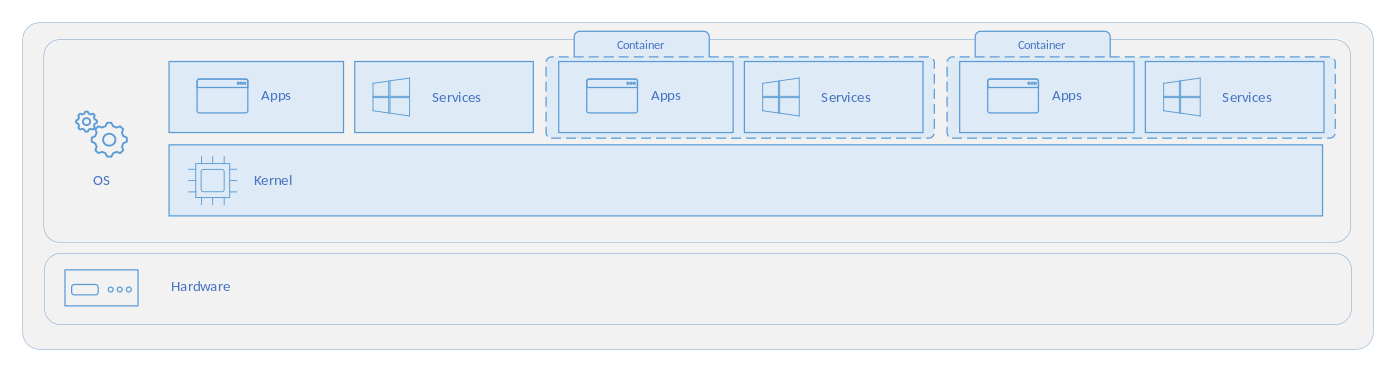
\includegraphics[width=\textwidth]{images/Diagramas/Esquema de Contenedores.png}
                    \caption{Arquitectura de los contenedores}
                    \label{fig:arquitectura-contenedores}
                \end{subfigure}
                
                \begin{subfigure}[h]{\textwidth}
                    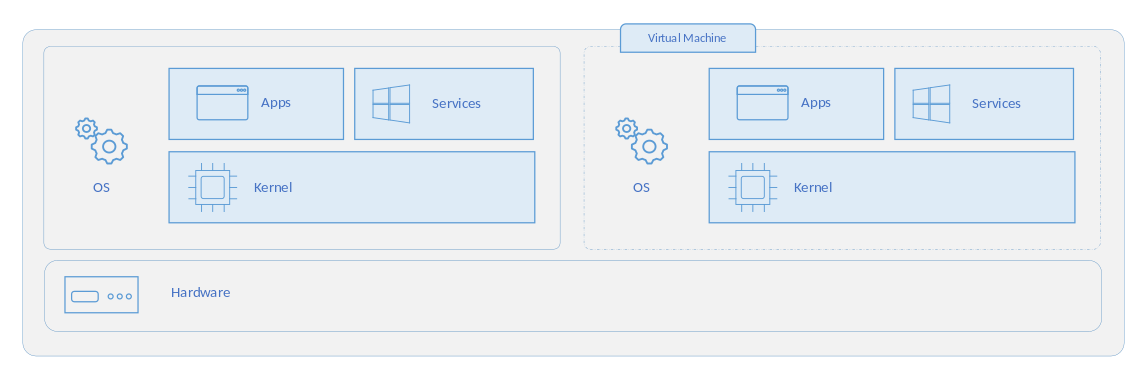
\includegraphics[width=\textwidth]{images/Diagramas/Esquema de MVs.png}
                    \caption{Arquitectura de las máquinas virtuales}
                    \label{fig:arquitectura-maquinasvirtuales}
                \end{subfigure}
                
                \caption{Diferencias entre contenedores y las máquinas virtuales}
                \label{fig:contenedores-vs-maquinasvirtuales}
            \end{figure}
            
            Docker funciona con imágenes, que son plantillas o modelos que contienen todos los componentes necesarios para ejecutar una aplicación en un contenedor, incluidos el código fuente, las librerías, los archivos de configuración y las dependencias del sistema. Estas imágenes pueden ser descargadas desde un registro centralizado llamado Docker Hub \cite{docker-hub} o construirse localmente por los desarrolladores.
            
            Una vez obtenida una imagen, se puede crear un contenedor a partir de ella, lo que implica crear una instancia de una aplicación y, por tanto, el entorno en el que se ejecuta. Los contenedores de Docker se pueden transferir fácilmente entre diferentes sistemas y entornos, lo que facilita la implementación y el escalado de aplicaciones.
            
            Además, Docker proporciona herramientas de administración de contenedores, como la capacidad de iniciar, detener, reiniciar y eliminar contenedores, así como la capacidad de monitorear su uso y rendimiento.

            Docker se ha empleado para crear los laboratorios de la plataforma; concretamente, cada laboratorio parte de un fichero Dockerfile cuya imagen es generada y almacenada en el sistema, y cuyos contenedores se crean y se destruyen bajo petición del usuario de la plataforma.
            
            \newpage

        \subsection{LAMP}

            Este es un acrónimo que se utiliza comúnmente en el mundo de los servidores para describir un conjunto de tecnologías de código abierto que se utilizan para construir y ejecutar aplicaciones web dinámicas.

            \begin{table}[!htbp]
                  \centering
                  
                  \begin{tabular}{|>{\centering\arraybackslash}m{3cm}|>{\centering\arraybackslash}m{3cm}|>{\centering\arraybackslash}m{8cm}|}
                        \hline
                        \textbf{Componente} & \textbf{Tipo} & \textbf{Descripción} \\
                        \hline
                        \hline
                        \textbf{Linux} & Sistema Operativo & Utilizado ampliamente en servidores web debido a su fiabilidad, seguridad y flexibilidad. \\
                        \hline
                        \textbf{Apache} & Servidor Web & Alojamiento de sitios web y aplicaciones web. \\
                        \hline
                        \textbf{MySQL} & RDBMS & Almacenamiento y recuperación de información para aplicaciones web. \\
                        \hline
                        \textbf{PHP} & Lenguaje de Programación & Creación de sitios web y aplicaciones web dinámicas. Procesa la lógica de la aplicación en el servidor. \\
                        \hline
                  \end{tabular}

                  \caption{Componentes habituales de la pila de software LAMP}
                  \label{table:lamp}
            \end{table}

            Esta pila ha sido ampliamente adoptada en la comunidad de desarrollo web y ha sido utilizada para crear una amplia variedad de aplicaciones, desde sitios web simples hasta aplicaciones web complejas y de alto tráfico.

            Además de los componentes principales mencionados anteriormente, la pila LAMP se puede personalizar y ampliar utilizando una variedad de tecnologías y herramientas adicionales, como frameworks de desarrollo, sistemas de caché, servidores de aplicaciones y más, según las necesidades específicas de cada proyecto.

            LAMP se ha empleado para crear la infraestructura de la plataforma web, y esta a su vez se ha desarrollado en un servidor local.

            \cleardoublepage

    
     
\chapter{Estado del arte}
    \label{cap:estado-arte}

    Actualmente existen diversas plataformas web de entrenamiento en ciberseguridad que ofrecen laboratorios y desafíos para mejorar las habilidades de seguridad ofensiva y defensiva de los usuarios.
    
    Dichas plataformas han experimentado un crecimiento en popularidad en los últimos años debido a la creciente demanda de profesionales en el campo de la seguridad informática y a la necesidad de mejorar las habilidades tanto de los estudiantes como de los profesionales en el campo.
    
    Estas plataformas varían en su enfoque y contenido, desde laboratorios que simulan entornos de la vida real hasta desafíos de explotación de vulnerabilidades, así como eventos de naturaleza más lúdica y competitiva como los retos de capturar la bandera, también conocidos como CTFs (\textit{Capture The Flag}).
    
    Algunas de estas plataformas han sido utilizadas en la educación, ya que permiten a los usuarios practicar y aplicar conceptos teóricos de seguridad informática en un entorno práctico, y también pueden ser útiles para empresas y organizaciones, ya sea para evaluar las habilidades de seguridad de los empleados o para mejorar la seguridad de sus sistemas.
    
    Respecto al futuro, se espera que continúen creciendo en popularidad y que aumente la variedad de laboratorios y desafíos que ofrecen, siendo muy probable que se produzca una mayor integración con otras tecnologías de inteligencia artificial, quizás dando lugar a una mejora en la calidad de esos desafíos y laboratorios mencionados, para que proporcionen una experiencia de usuario más personalizada.
    
    A continuación se presenta una breve descripción de algunas de las plataformas más populares actualmente, donde se muestran sus similitudes y sus diferencias:
    
    \newpage
    
    
    \section{Hack The Box}
    
        Plataforma web de entrenamiento que ofrece más de 200 desafíos y laboratorios de amplia variedad, diseñados para mejorar las habilidades de seguridad ofensiva y defensiva de los usuarios. Hack The Box se ha vuelto \textbf{la plataforma más popular} en la comunidad de seguridad informática debido a su \textbf{enfoque en la calidad de los desafíos y laboratorios} y su \textbf{comunidad activa de usuarios}.
        
        Sus retos abarcan desde desafíos básicos de hacking hasta laboratorios avanzados, y también ofrece una función llamada \textit{Boxes} diseñada para simular entornos de la vida real, como redes empresariales, que contienen múltiples vulnerabilidades que los usuarios pueden explotar para ganar acceso a sistemas y obtener información confidencial.
        
        \begin{figure}[h]
            \centering

            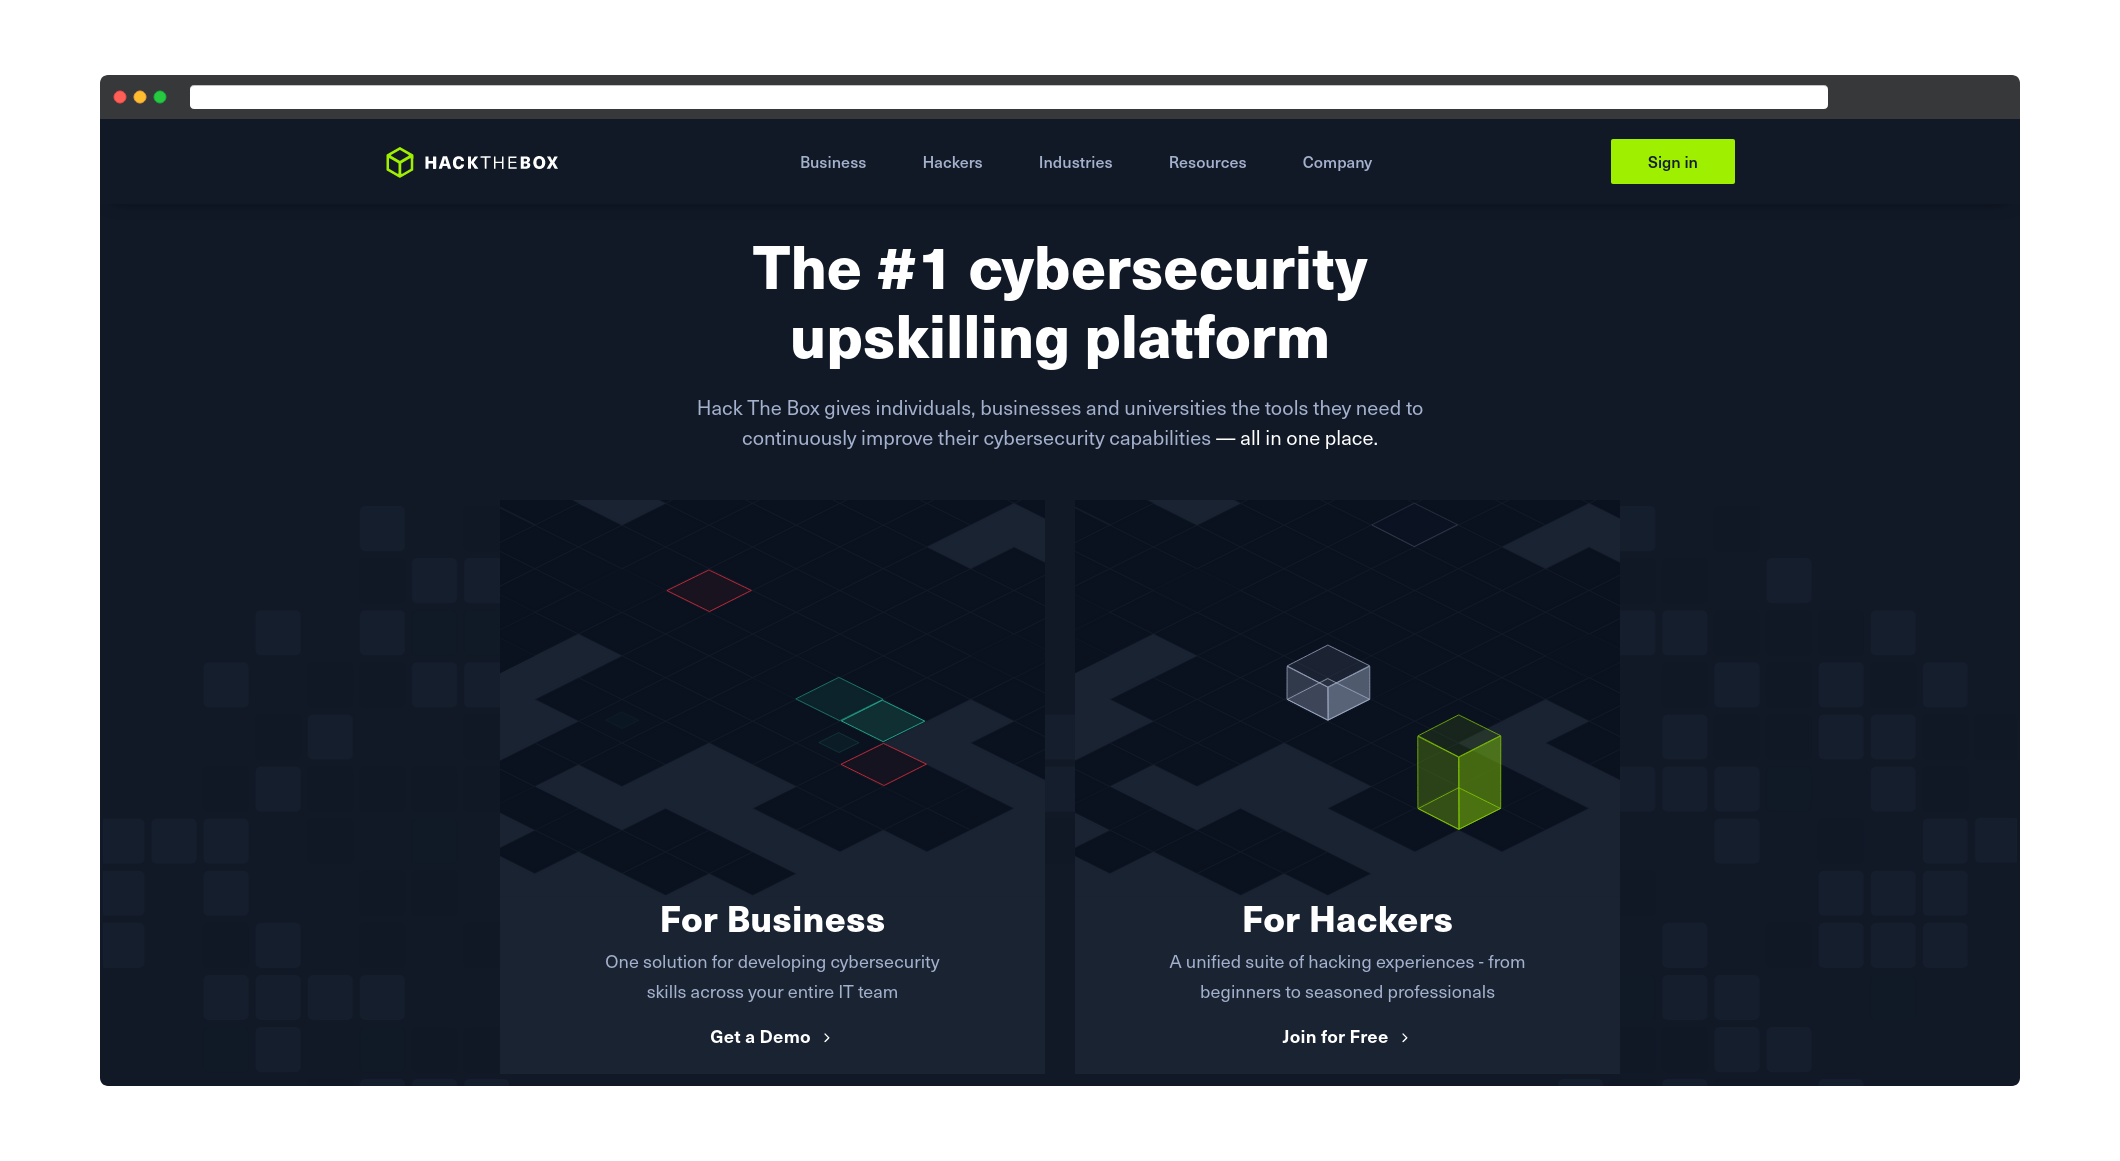
\includegraphics[width=\textwidth]{images/Capturas/Web de HTB.png}

            \caption{Web de Hack The Box}
            \label{fig:HTB-web}
        \end{figure}
        
        Una de las características más interesantes de esta plataforma es su enfoque en el hacking ético, ya que se fomenta una cultura de hacking responsable y legal y requiere que los usuarios acepten un código de conducta antes de unirse. Los usuarios también son alentados a informar sobre cualquier vulnerabilidad que encuentren en la plataforma.
        
        Hack the Box ofrece diferentes \textbf{planes de suscripción} para los usuarios interesados en acceder a su contenido:
        
        \begin{itemize}
            \item \textbf{Plan gratuito}: acceso limitado a una selección de desafíos y laboratorios, pero no incluye acceso a los \textit{boxes}.
        
            \item \textbf{Plan VIP}: acceso completo a la plataforma (todos los laboratorios, desafíos y \textit{boxes} disponibles).
        
            \item \textbf{Planes empresariales}: personalizados para empresas y organizaciones que deseen utilizar la plataforma para la formación y evaluación de sus empleados en seguridad informática.
        \end{itemize}
        
        \newpage

    
    \subsection{HTB Academy}
    
        Esta es una iniciativa de Hack The Box que también ofrece formación, pero al contrario que Hack The Box, centrada en la práctica y el desafío en tiempo real, HTB Academy \textbf{se enfoca en la enseñanza práctica de habilidades a través de cursos y laboratorios}.
        
        \begin{figure}[h]
            \centering

            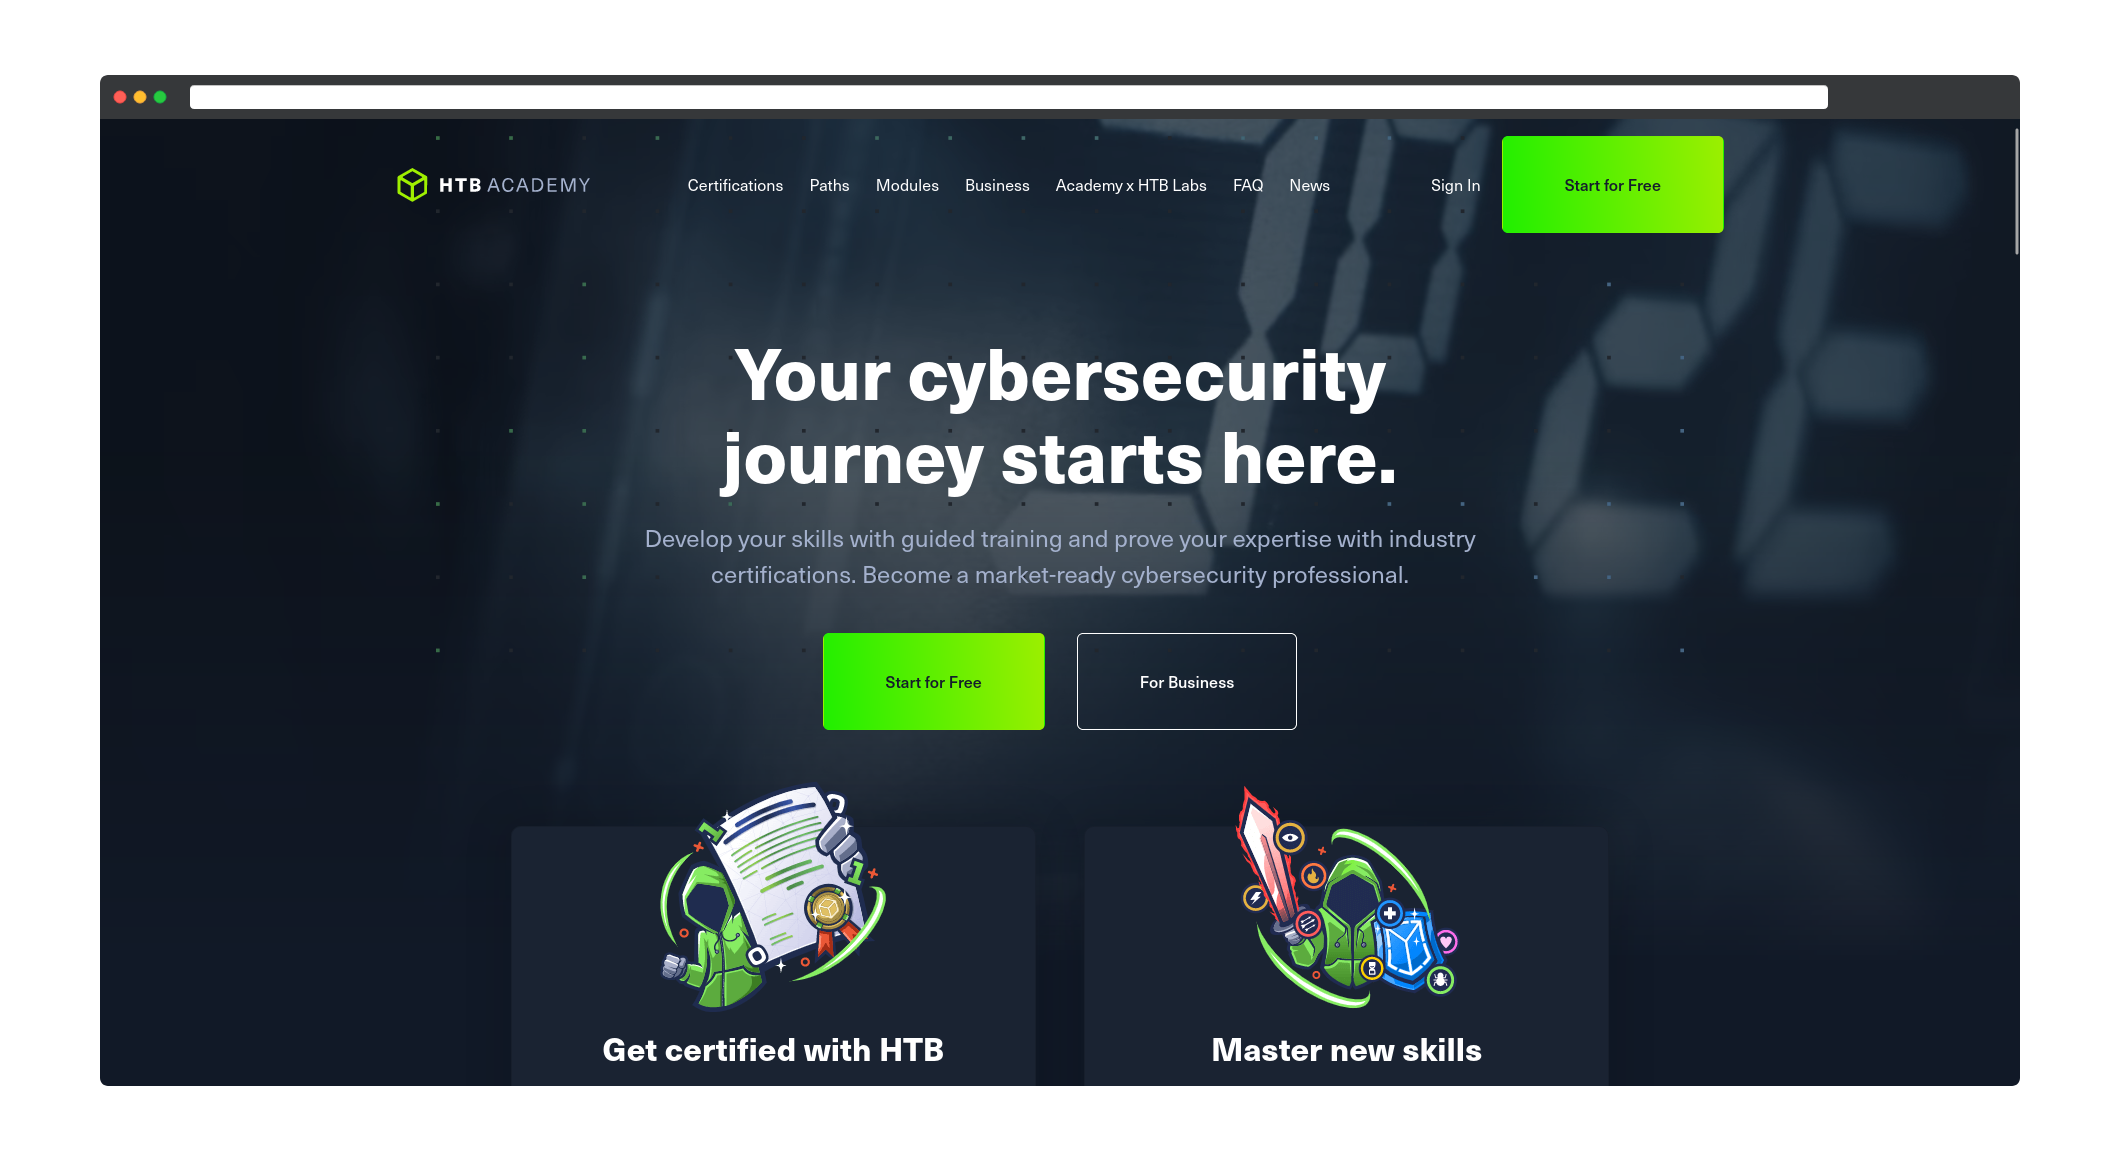
\includegraphics[width=\textwidth]{images/Capturas/Web de HTB Academy.png}
            
            \caption{Web de HTB Academy}
            \label{fig:HTB-Academy-web}
        \end{figure}
        
        Los cursos están diseñados para ser prácticos, con una orientación en la experimentación activa que permite a los usuarios adquirir habilidades en la práctica, y no solo a través de la teoría.
        
        Cubren una amplia gama de temas, desde los fundamentos de la seguridad informática hasta temas avanzados como el análisis de malware, el hacking web y la ingeniería inversa, ya que están diseñados para ser accesibles desde principiantes hasta expertos en el sector.
        
        Esta plataforma cuenta con los mismos tipos de \textbf{planes de suscripción} que Hack The Box: gratuito, VIP y empresarial; aunque es importante destacar que tanto Hack The Box como HTB Academy son servicios diferentes, por lo que \textbf{los planes de ambas plataformas son completamente independientes entre sí}.
        
        \newpage
    
    
    \section{TryHackMe}
    
        Plataforma de aprendizaje de ciberseguridad basada en la experimentación activa, que proporciona una variedad de entornos de laboratorio virtuales y desafíos prácticos para ayudar a los usuarios a aprender y mejorar sus habilidades en seguridad informática. Su contenido se encuentra organizado en \textbf{diferentes rutas de aprendizaje} que permiten a los usuarios desarrollar su conocimiento de forma estructurada.
        
        \begin{figure}[h]
            \centering

            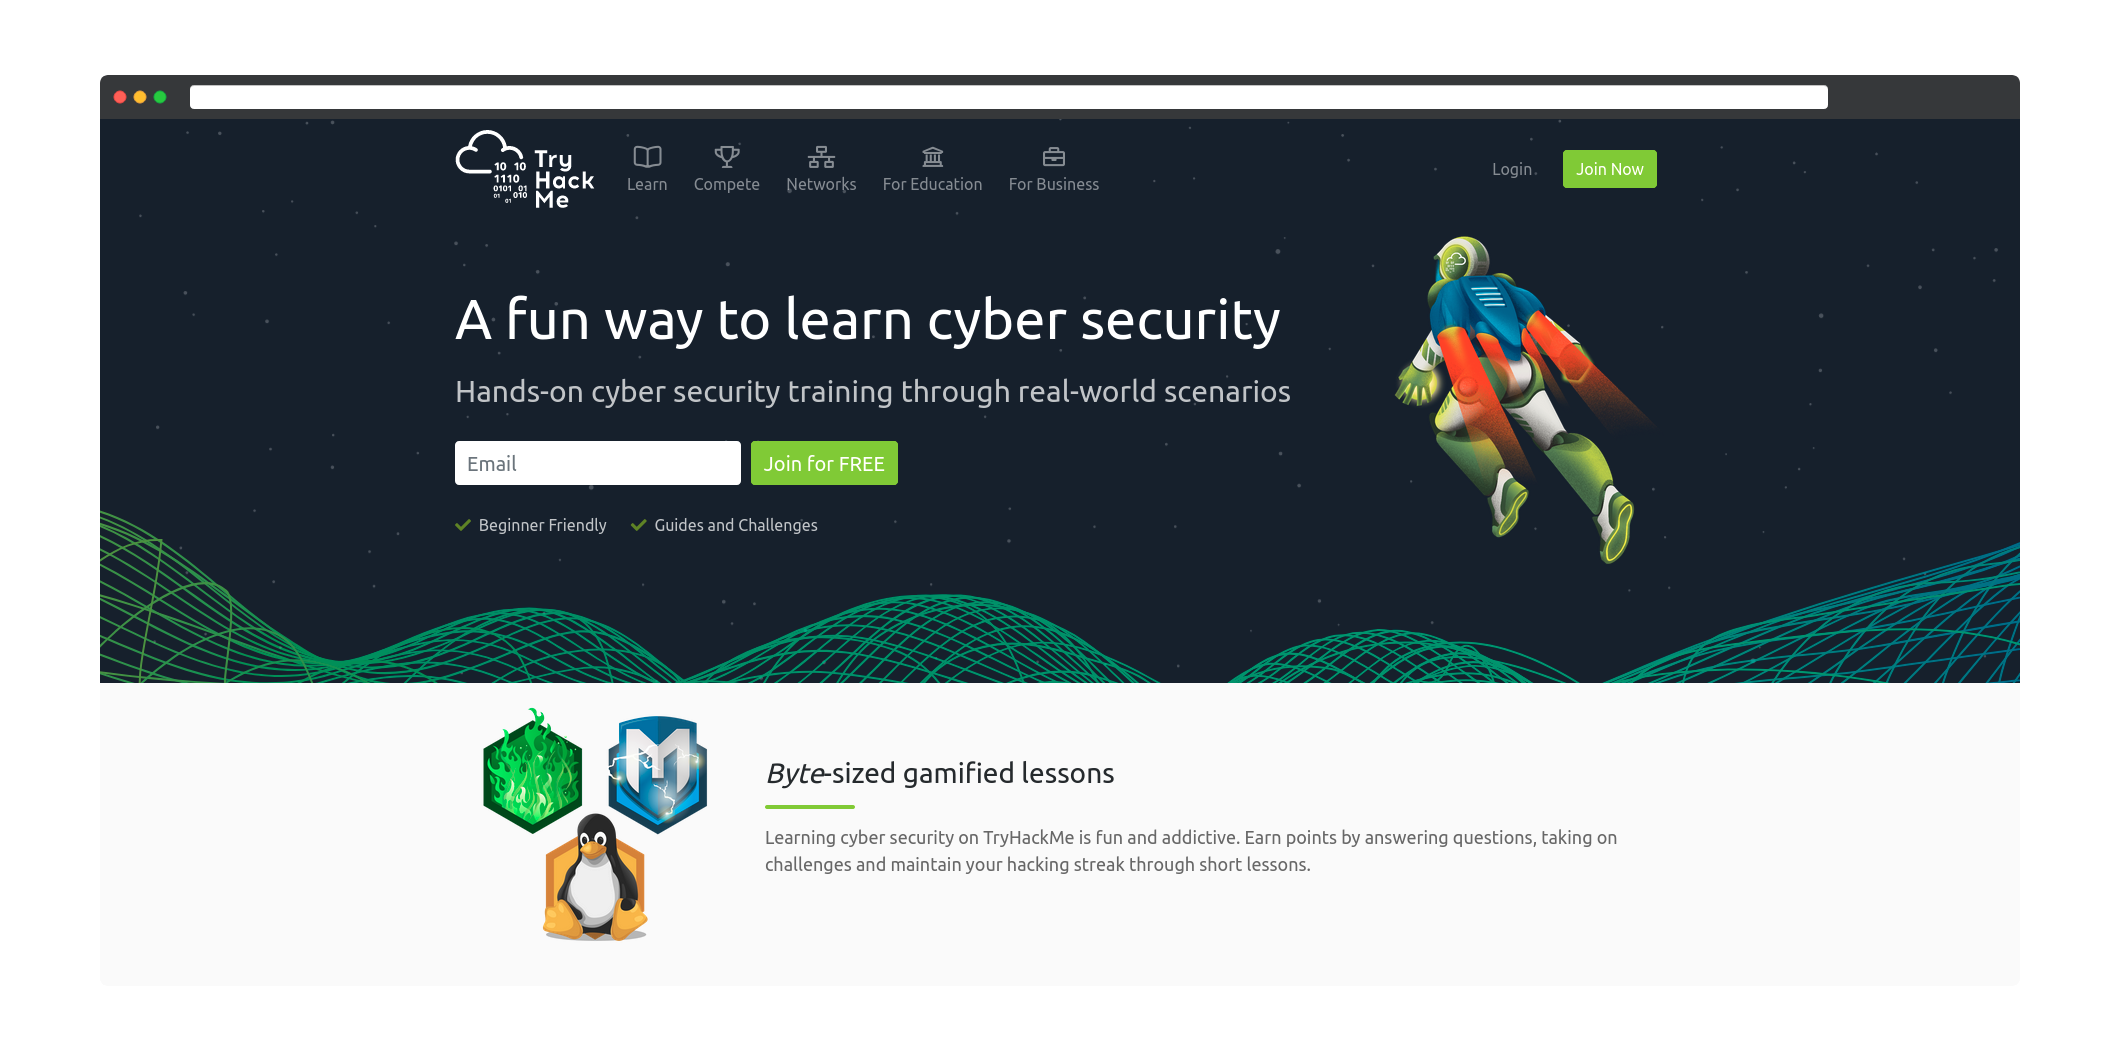
\includegraphics[width=\textwidth]{images/Capturas/Web de THM.png}

            \caption{Web de TryHackMe}
            \label{fig:THM-web}
        \end{figure}
        
        La plataforma también cuenta con una comunidad activa y una función de \textit{gamificación} que proporciona una experiencia de aprendizaje más interactiva y entretenida, permitiendo que los usuarios puedan competir entre ellos, ganando puntos y recompensas por completar desafíos y resolver problemas de seguridad.
        
        TryHackMe ofrece diferentes \textbf{planes de suscripción} para los usuarios interesados:
        
        \begin{itemize}
            \item \textbf{Plan gratuito}: acceso limitado a una selección de desafíos y laboratorios.
        
            \item \textbf{Plan premium}: acceso completo a la plataforma (todos los laboratorios y desafíos).
        
            \item \textbf{Planes empresariales}: personalizados para empresas y organizaciones que deseen utilizar la plataforma para la formación y evaluación de sus empleados en seguridad informática.
        \end{itemize}
        
        \newpage
    
    
    \section{VulnHub}
    
        Plataforma de laboratorios que proporciona una gran cantidad de \textbf{máquinas virtuales vulnerables que los usuarios pueden descargar} y configurar en sus propios entornos de laboratorio para luego explotar sus vulnerabilidades. Cada máquina virtual cuenta con descripción detallada de su objetivo y una guía paso a paso para ayudar a los usuarios en su proceso de aprendizaje.
        
        \begin{figure}[h]
            \centering

            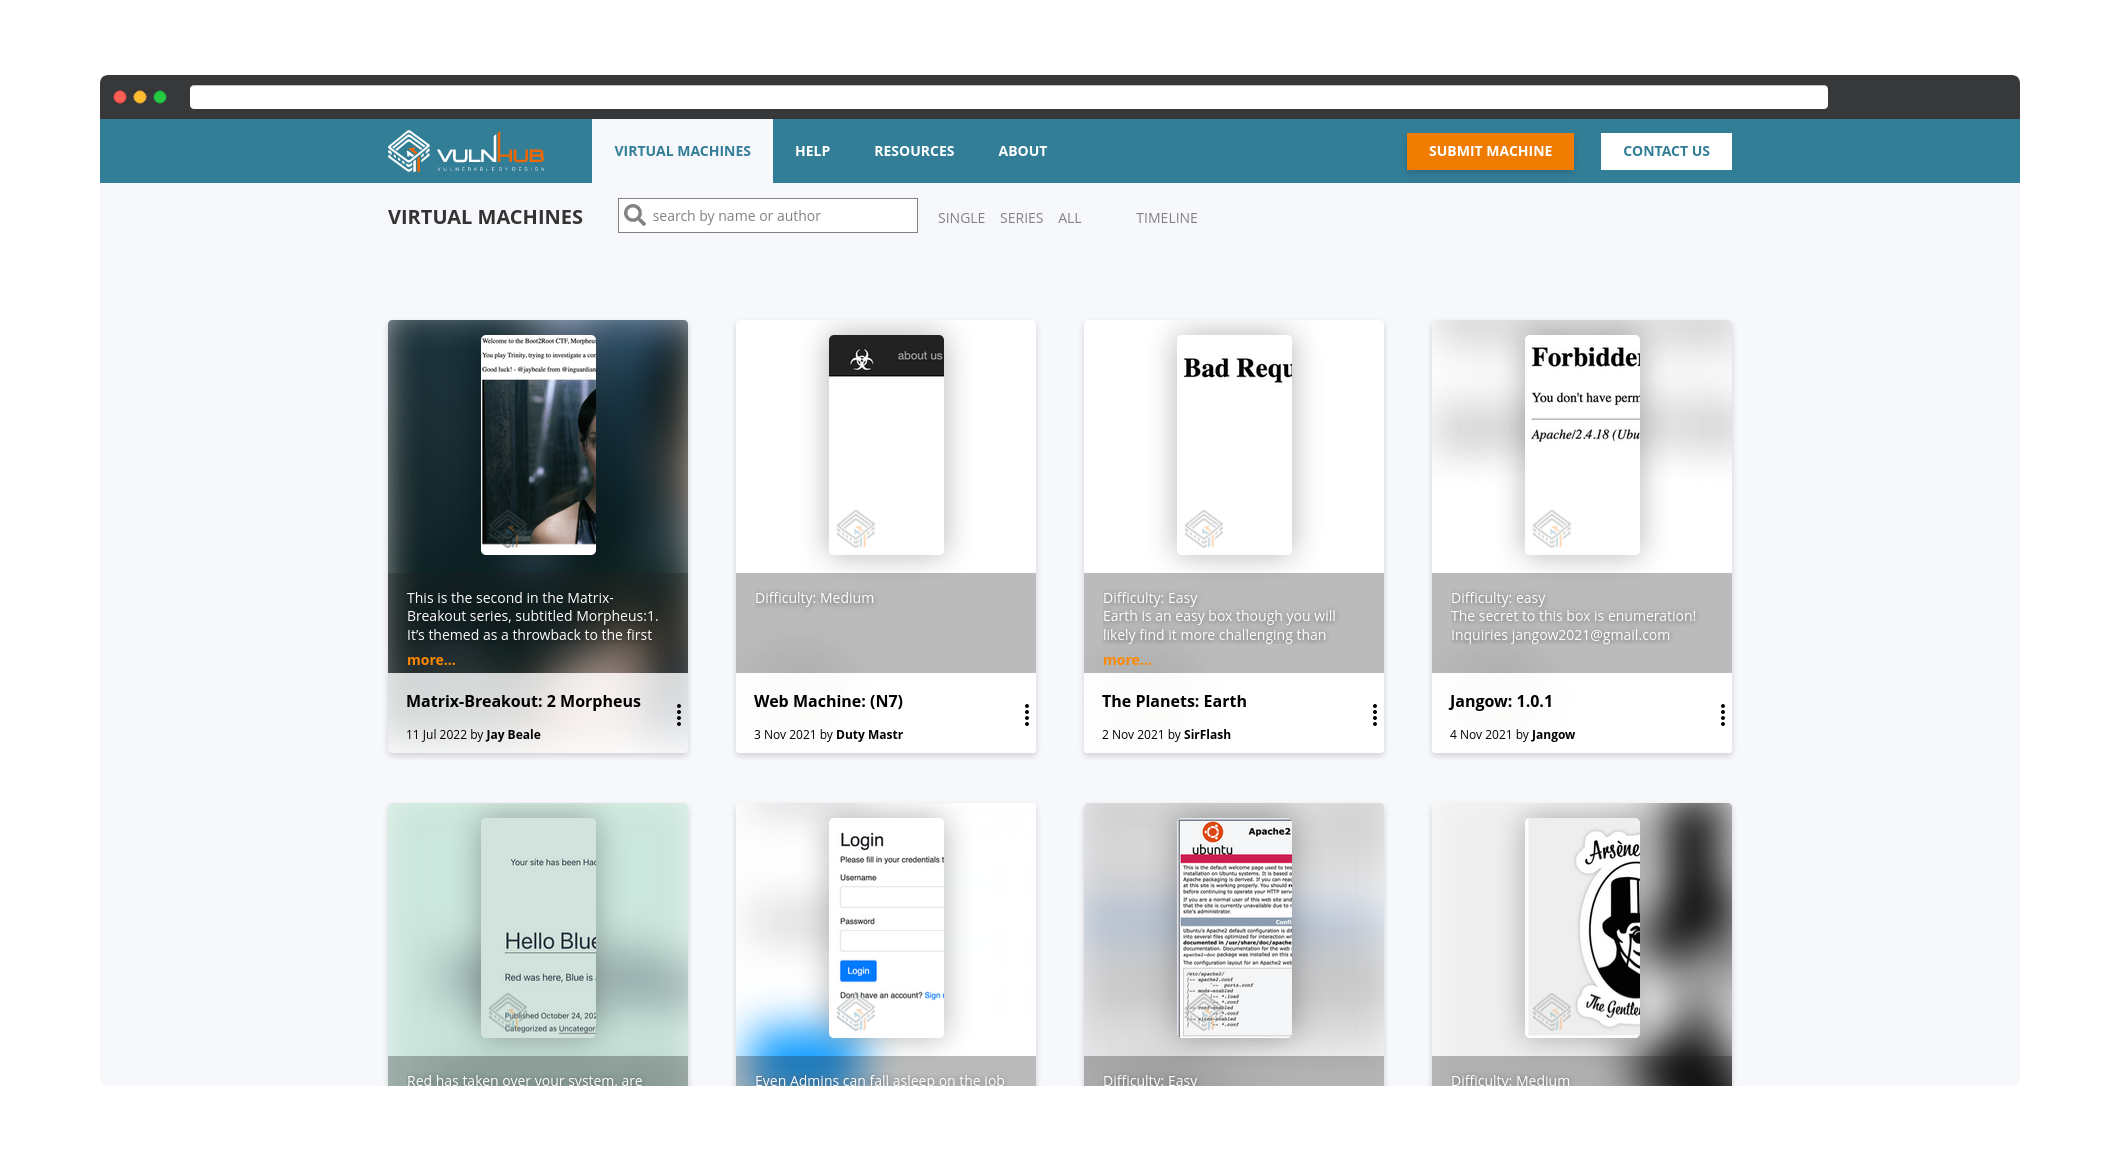
\includegraphics[width=\textwidth]{images/Capturas/Web de VulnHub.png}

            \caption{Web de VulnHub}
            \label{fig:VulnHub-web}
        \end{figure}
        
        Estos desafíos son diseñados por la comunidad, y la plataforma también ofrece la opción de que los usuarios puedan crear y compartir sus propios desafíos y máquinas virtuales.
        
        Al contrario de lo que sucede con otras plataformas, entre ellas Hack The Box y TryHackMe mencionadas anteriormente, \textbf{esta plataforma es completamente gratuita} y todo su contenido está construido por y para los usuarios.
        
        \newpage
    
    
    \section{OverTheWire}
    
        Plataforma de laboratorios \textbf{diseñada de manera progresiva}, donde los usuarios pueden avanzar en su aprendizaje de forma gradual, comenzando con los niveles más fáciles y avanzando hacia los más complejos. Cada nivel de desafío presenta un objetivo diferente, haciendo que los usuarios deban usar su ingenio y habilidades en seguridad informática para resolver los desafíos y avanzar al siguiente nivel.
        
        \begin{figure}[h]
            \centering

            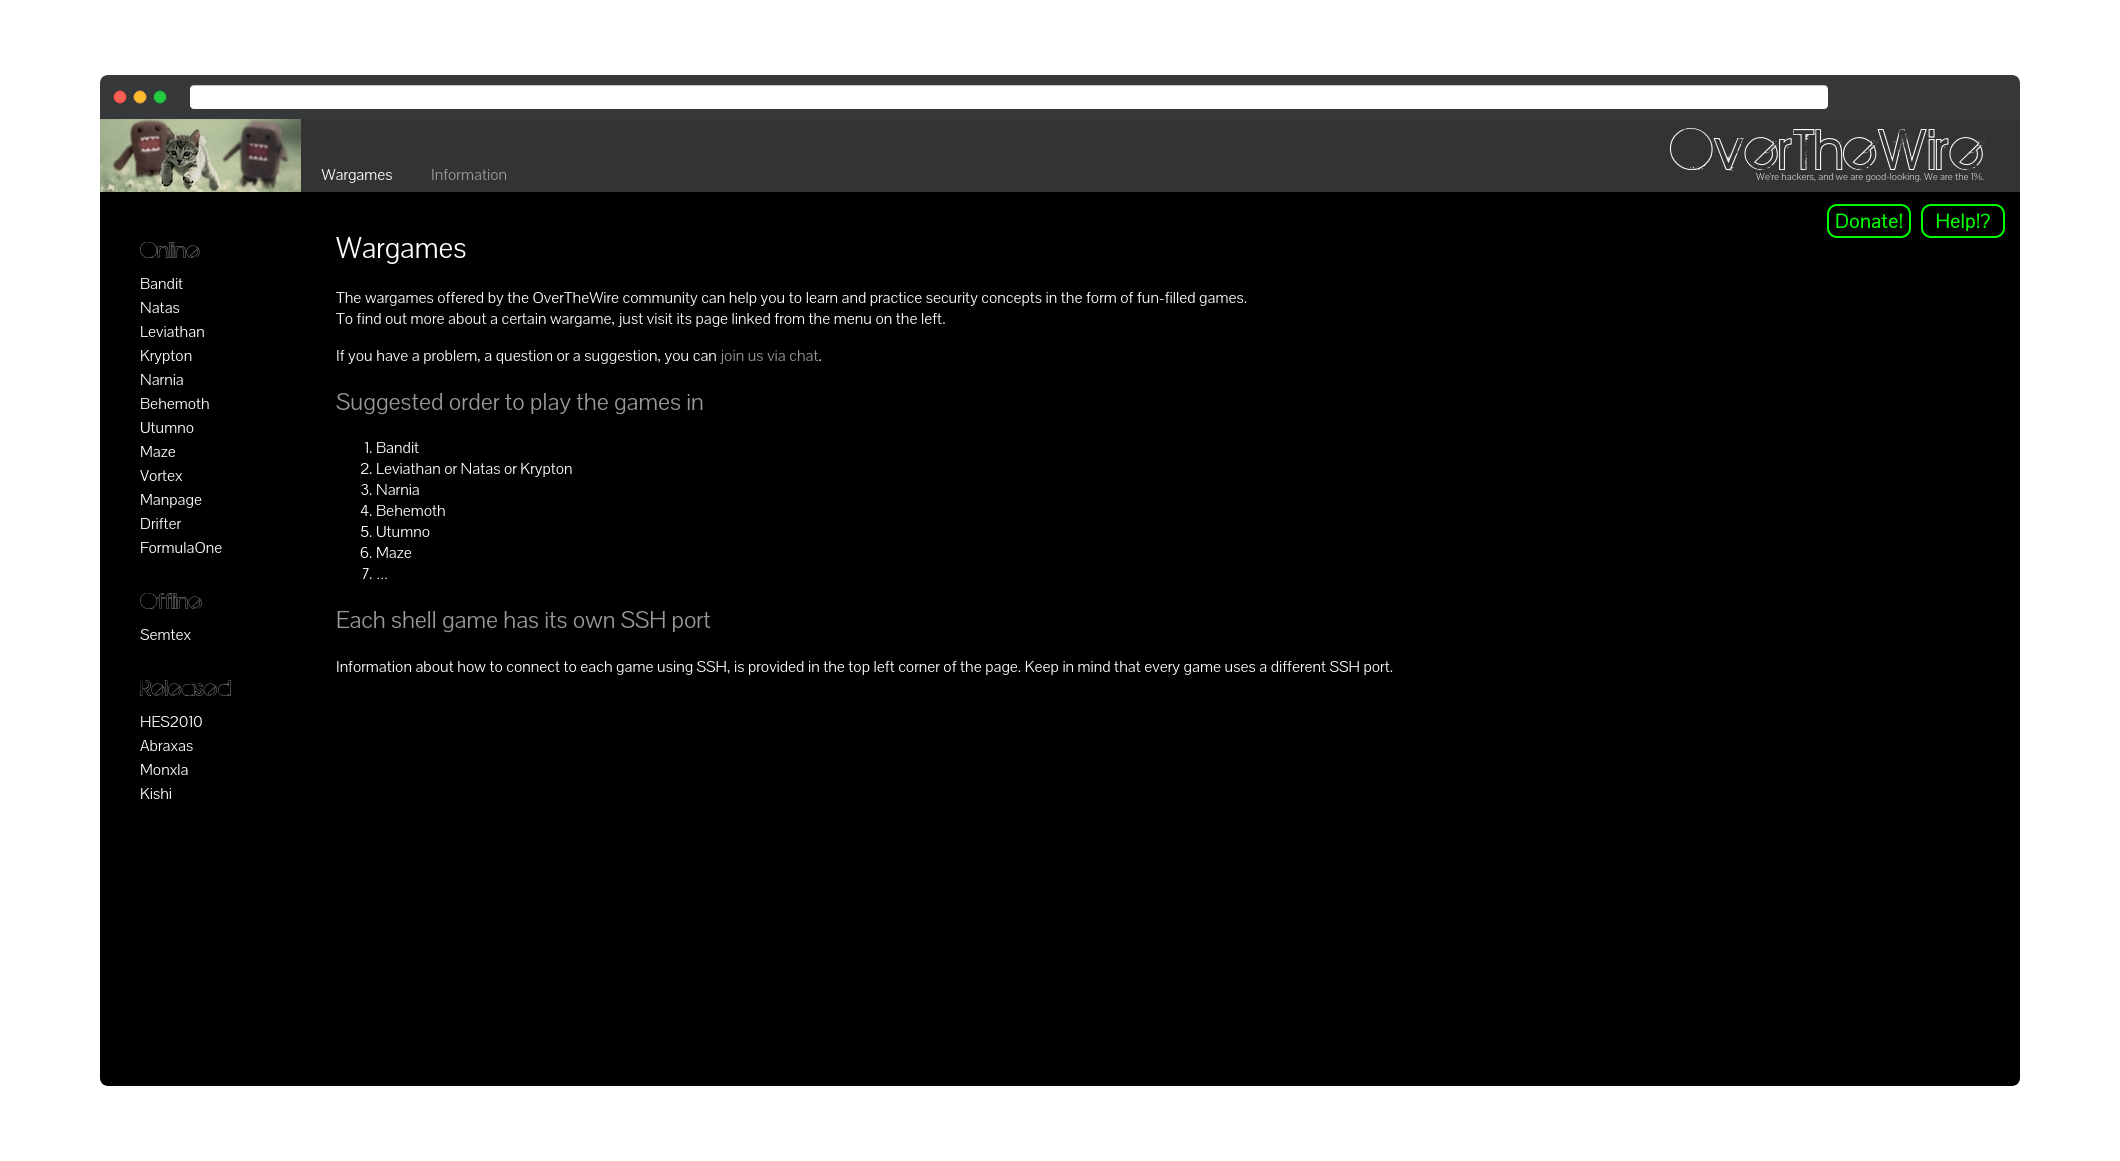
\includegraphics[width=\textwidth]{images/Capturas/Web de OverTheWire.png}

            \caption{Web de OverTheWire}
            \label{fig:OverTheWire-web}
        \end{figure}
        
        Uno de los aspectos únicos de OverTheWire es que los desafíos están diseñados para simular situaciones del mundo real, lo que permite a los usuarios adquirir habilidades prácticas y relevantes para el mundo laboral de la ciberseguridad, pudiendo aplicar lo aprendido a situaciones reales y utilizar sus habilidades para asegurar sistemas y aplicaciones.
        
        Al contrario de lo que sucede con otras plataformas, entre ellas Hack The Box y TryHackMe mencionadas anteriormente, \textbf{esta plataforma es completamente gratuita} y todo su contenido está construido por y para los usuarios.
        
        \cleardoublepage
    
    

\chapter{Investigación previa}
    \label{cap:investigacion-previa}

    \section{Proceso creativo}
        \label{sec:proceso-creativo}

        Antes de comenzar a desarrollar el proyecto, resulta importante saber de forma más específica \textit{qué} se quiere llevar a cabo, y una vez decidio el objetivo, analizar las posibles opciones para conseguirlo.
        
        Ya se realizó una investigación previa sobre las diferentes plataformas de aprendizaje de ciberseguridad existentes -descritas en el Estado del Arte (capítulo \ref{cap:estado-arte})- con el objetivo de analizar sus características y funcionalidades.
        
        La mayoría -y más conocidas- de estas plataformas son CTFs (Capture The Flag), y aunque son muy útiles para poner en práctica los conocimientos adquiridos, no suelen ofrecer un entorno de aprendizaje guiado, sino que el usuario debe resolver los desafíos por su cuenta, sin ningún tipo de documentación que le ayude a resolverlos, más allá de las pistas que ofrezca la propia plataforma o las soluciones que hayan publicado otros usuarios en Internet.

        Sin embargo, esto no siempre es así, ya que como se vió en el apartado anterior, Try Hack Me \cite{tryhackme} ofrece tanto retos instructivos como retos puramente prácticos y competitivos; mientras que Hack The Box \cite{hackthebox}, la plataforma más reconocida, ha sido capaz de lanzar su propia plataforma educativa con retos guiados: HTB Academy \cite{hackthebox-academy}.

        Teniendo eso en cuenta, se plantearon las siguientes ideas para afrontar el proyecto.

        \subsection{Plataforma de CTFs}

            La primera idea planteada fue, precisamente, replicar una plataforma de CTFs (Capture The Flag). Esta versión del proyecto se centraría más en enseñar distintos conceptos de la ciberseguridad al usuario, acompañados de una serie de retos que pondrían a prueba los conocimientos adquiridos, parecido a las plataformas TryHackMe y HTB Academy mencionadas en el apartado anterior.

            Esta idea fue descartada porque ya existen muchas plataformas de CTFs y se pretendía hacer algo distinto con este proyecto. Se requería un entorno de aprendizaje guiado y como se mencionó anteriormente, los CTFs no suelen ofrecerlo.

        \subsection{Plataforma como portal de descargas}

            Tomando como ejemplo los retos descargables de la Academia Hacker de Incibe \cite{retos-INCIBE}, se planteó la posibilidad de crear máquinas virtuales y alojarlas en el servidor a modo de elementos descargables.
            
            Es decir, la plataforma contaría con un sitio web que ofrecería información documentada sobre distintos conceptos de ciberseguridad, pero la virtualización se llevaría a cabo por el propio usuario en su equipo, experimentando localmente.

            Esta idea también fue descartada porque plantea un gran problema de fricción entre el usuario y el objetivo de la plataforma: no existiría la posibilidad de ofrecer un entorno de trabajo en el que el usuario pudiera interactuar con los laboratorios de forma remota y con herramientas aisladas, sino que este debería descargar y configurar un hypervisor, o instalar Docker para acceder a los entornos de prueba en su equipo. Debido a esto, se perdería esa esencia de minimalismo y sencillez que debería ofrecer la plataforma.
            
            Además, plantea otros problemas relacionados con el espacio de almacenamiento (tanto en el servidor como en el equipo del usuario).
            
            También puede ser útil incluir en la plataforma de una guía introductoria a la configuración de una máquina virtual para tests de intrusión (pentesing) con Kali Linux, ya que si bien no es objeto de este proyecto que los usuarios aprendan sobre virtualización, no se puede ignorar el hecho de que es necesario el uso de máquinas virtuales para el sector de la ciberseguridad.

        \subsection{Plataforma de laboratorios}

            Por último, se planteó crear una plataforma de laboratorios con la que el usuario pudiera acceder a distintos entornos de forma remota, sin necesidad de descargar ni configurar nada en su equipo. La plataforma estaría compuesta de un sitio web donde estaría recogida la documentación, mientras que el servidor alojaría los entornos virtualizados asociados a dicha documentación.
            
            La principal diferencia y rasgo a destacar de este planteamiento es que los laboratorios actuarían como \textit{sandboxes}; es decir, ofrecería al usuario un entorno con herramientas preinstaladas en el caso de querer hacer sus propias pruebas sobre un concepto en específico.

            Esta idea fue la que más se acercaba a los objetivos del proyecto, y por tanto fue la que se escogió para su desarrollo: solventaba las fricciones de las ideas anteriores, y además ofrecía un entorno de aprendizaje guiado y práctico, que era el objetivo principal del proyecto.

        \subsection{Docker para los laboratorios}

            Docker, descrito en la sección \ref{sec:docker}, permitiría la creación de contenedores para los distintos laboratorios, siendo una solución mucho más ligera que el uso de máquinas virtuales.
                
            Esta idea surgió a partir del artículo \textit{Cyber Security Testbeds and Malware Testing} \cite{securitylab-malware-analysis} de la Universidad de Trento, donde un grupo de investigación realizaban un estudio sobre los efectos de un \textit{exploit} de una aplicación sobre varias versiones de la misma y usada en distintos entornos de desarrollo.

            \begin{quotation}
                
                Given a software environment $E$, an exploit $X$ that successfully subverts an application $A$, that is running on $E$:
                
                \begin{itemize}
                    \item Will $X$ be successful on an application $A$ running on another environment $E'$?
                    \item Will $X$ be successful on another version of $A$, $A'$, running on $E$?
                    \item Will $X$ be successful on another version of $A$, $A'$, running on $E'$?
                \end{itemize}

            \end{quotation}

            Para ello, el grupo de investigación desarrolló un conjunto de pruebas a partir de contenedores, usando combinaciones de un conenedor principal junto a contenedores secundarios.

            \begin{quote}

                Instead of creating separate virtual machines for every application/configuration we use the Linux Containers technology that provides virtualization capabilities on the operation system level. \[...\] We use Docker to implement two types of containers: (1) software-specific that contain operating system, webserver and database engine; (2) application-specific that is build on top of a desired software-specific container and also encapsulates the application files. The figure on the right shows an example Wordpress3.2 application container that has been built on top of the “ubuntu-apache-mysql” software container.

            \end{quote}

            Y la figura que representa dicho planteamiento es la siguiente:

            \begin{figure}[htbp]
                \centering

                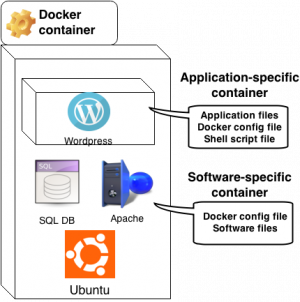
\includegraphics[scale=0.75]{images/Diagramas/Articulo.png}

                \caption{Ejemplo de contenedor extraído del artículo \cite{securitylab-malware-analysis}}
                \label{fig:articulo}
            \end{figure}

            \newpage
                
            \subsubsection{Solución del artículo}

                La estructura descrita en el artículo se forma a través del uso de la tecnología de contenedores de Linux, alojando cada aplicación y configuración de software en un contenedor.

                Una posible réplica de ese mecanismo podría realizarse de la siguiente forma:

                \begin{enumerate}

                    \item \textbf{Instalar Docker en el sistema operativo}
                    
                    Realizable siguiendo las instrucciones de instalación en el sitio web oficial de Docker.
                
                    \item \textbf{Crear imágenes específicas del software}
                    
                    Realizable utilizando un archivo Dockerfile que describa la configuración y los componentes que deben incluirse en dicha imagen.

                    \item \textbf{Crear un contenedor específico de la aplicación}

                    Para crear este tipo de contenedor, se debe construir sobre un contenedor específico del software previamente creado; para ello, se deben encapsular los archivos de la aplicación dentro del contenedor específico del software.

                    \item \textbf{Ejecutar contenedores}
                    
                    Una vez creados los contenedores específicos del software y de la aplicación, pueden ejecutarse con el comando \texttt{docker run} de Docker.

                \end{enumerate}
                
                \begin{figure}[!htbp]
                    \centering

                    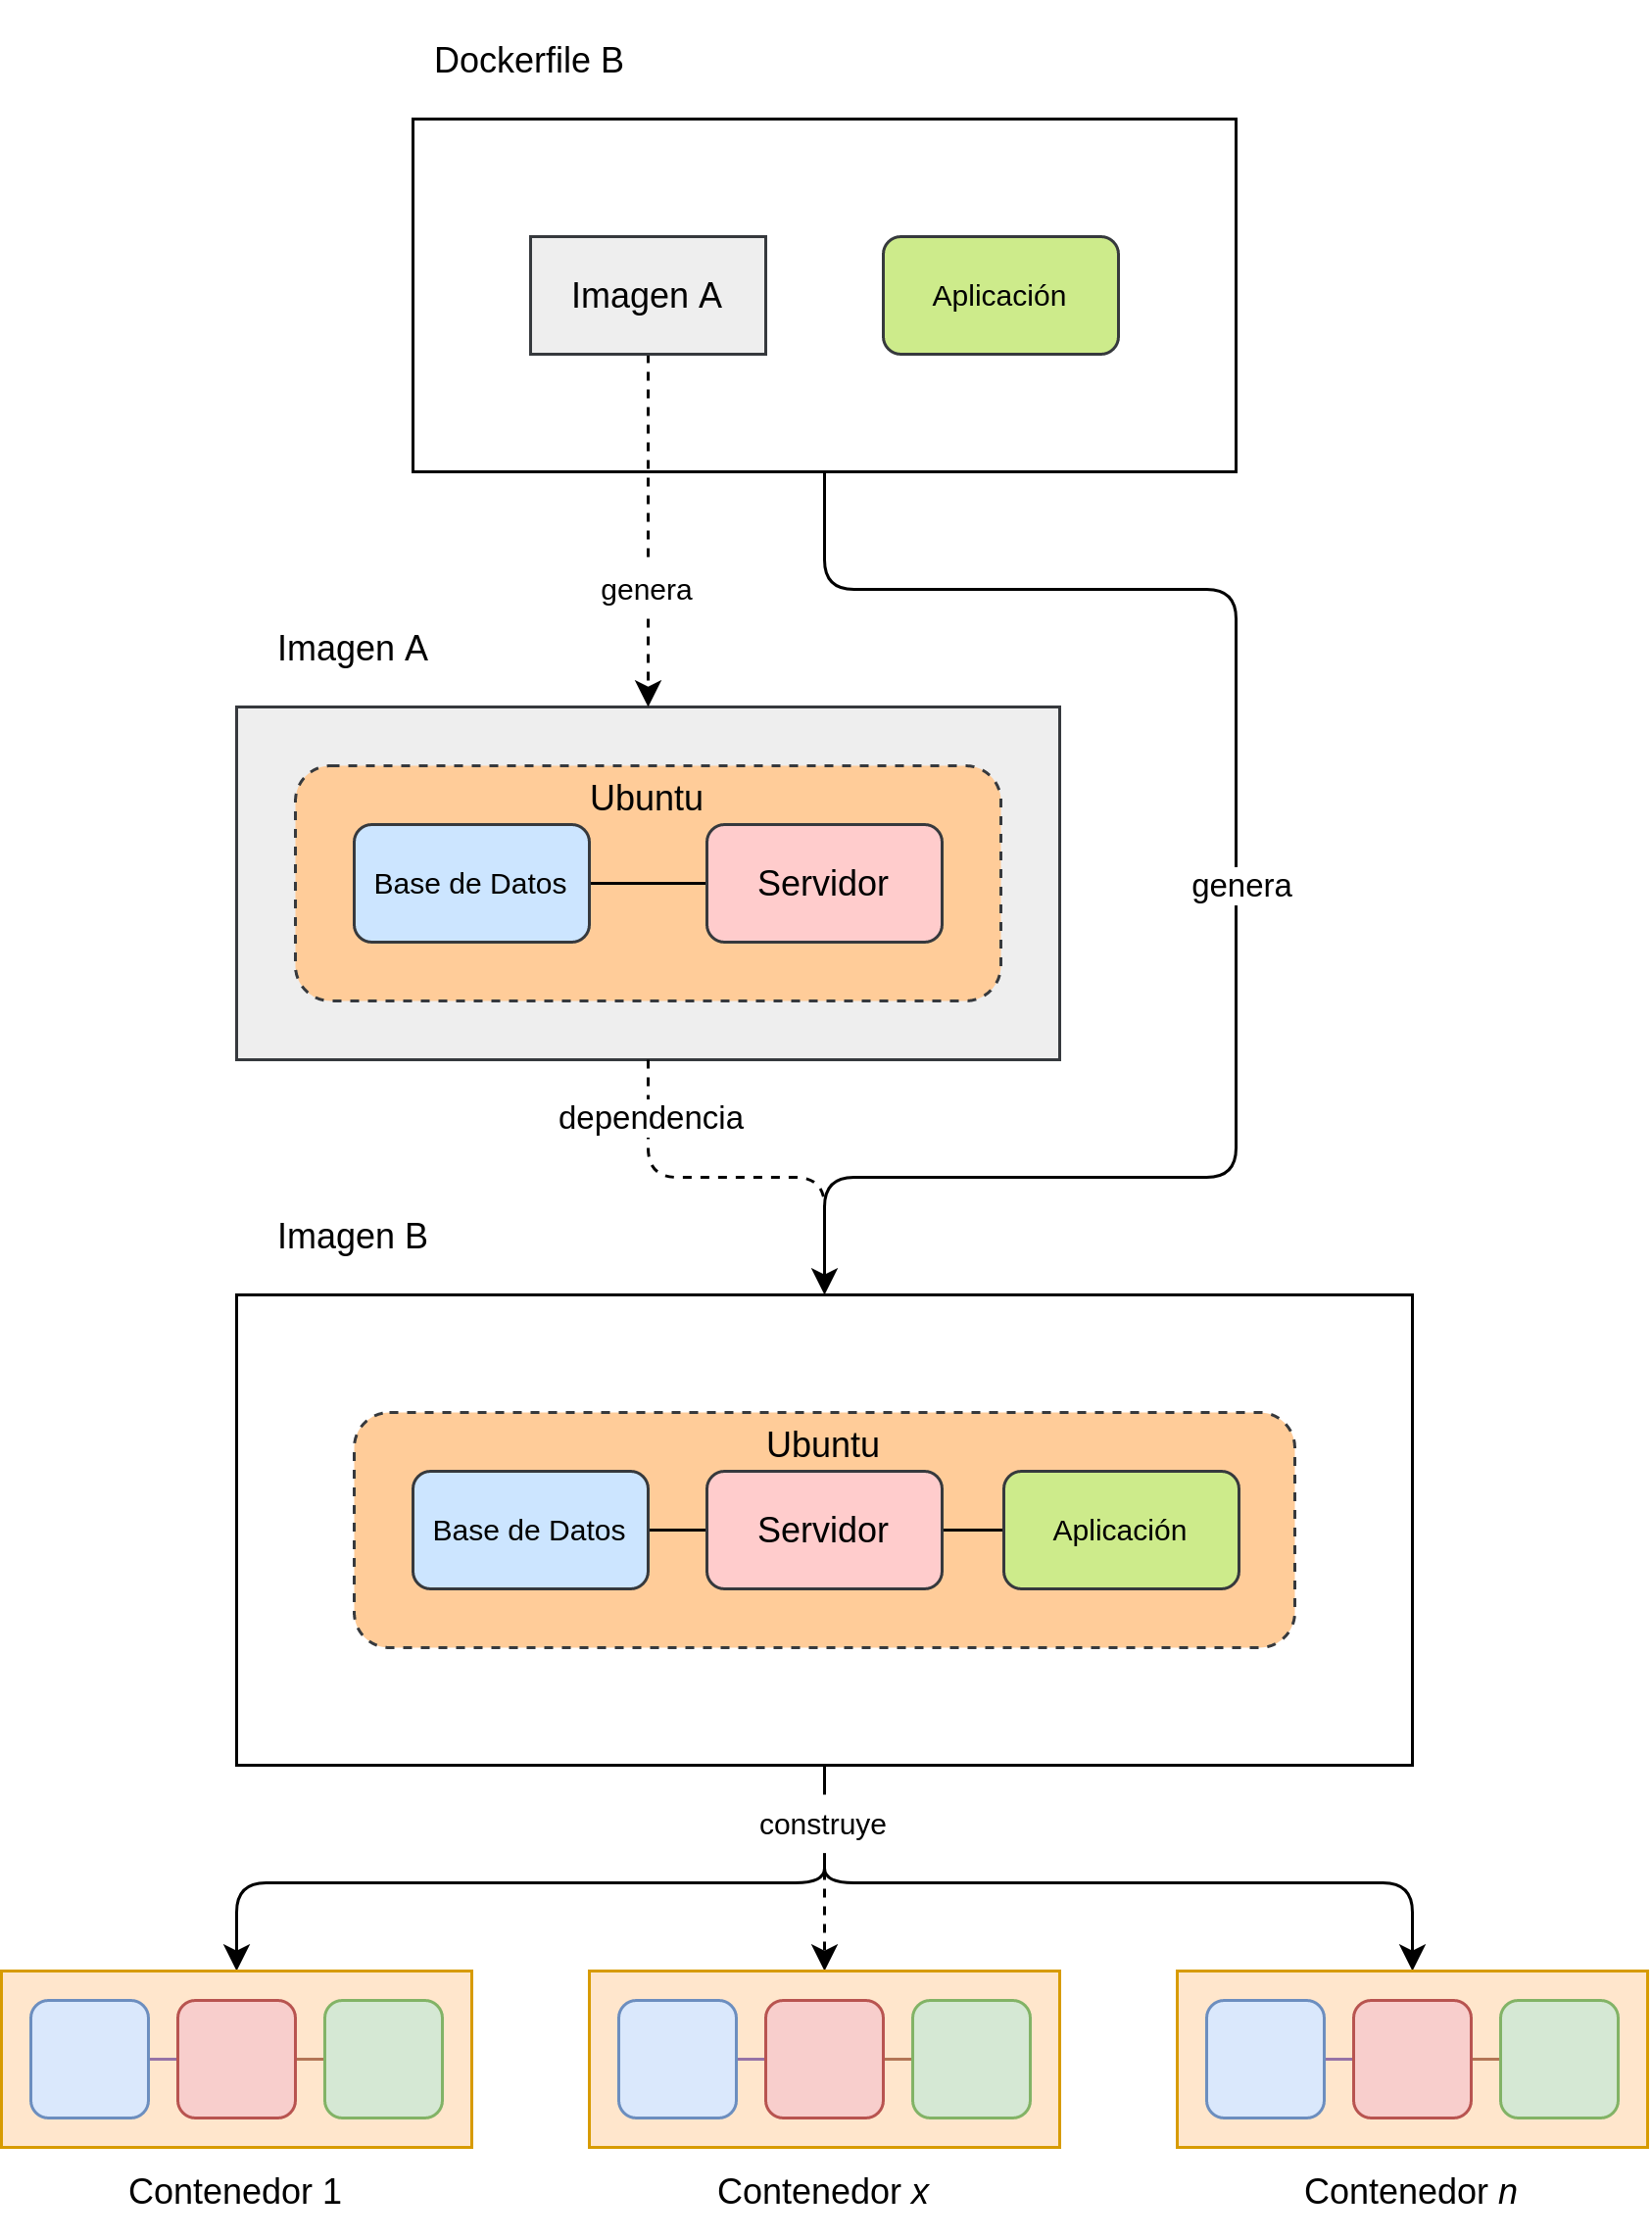
\includegraphics[scale=0.15]{images/Diagramas/Contenedor B.png}

                    \caption{Creación de contenedores a partir de una imagen $A$ padre}
                    \label{fig:contenedor-hijo}
                \end{figure}
                
                \newpage

                En el paso 2, se crea una imagen específica del software a partir de un archivo Dockerfile que describe la configuración y los componentes que deben incluirse en los contenedores resultantes de dicha imagen.

                En el paso 3, se crea una imagen específica de la aplicación que se construye sobre la imagen del software previamente creada; es decir, se crea una nueva imagen que constituye una capa de configuración adicional sobre la configuración de la propia imagen del software, que actua como base. Esta nueva imagen encapsula los archivos de la aplicación y se crea también a partir de un archivo Dockerfile.

                El resultado final es un contenedor específico de la aplicación que reutiliza el sistema operativo y los componentes incluidos en la imagen del software, pero que añade los archivos específicos para el funcionamiento de la aplicación.

                A continuación se muestran dos ejemplos de pseudo-código de ficheros Dockerfile que describen la creación de imágenes específicas del software y de la aplicación, respectivamente.

                \paragraph{Imagen padre} Este Dockerfile establece una configuración básica del sistema operativo, y se instala el software necesario para el funcionamiento de la aplicación. Su propósito es servir como base para la creación de la imagen hija, que contendrá los archivos de la aplicación y se construirá sobre la imagen padre:
                \\

                \begin{lstlisting}[style=dockerfile_style, caption={Dockerfile de una imagen principal (padre)}]
    # Se usa una imagen base con ubuntu
    FROM ubuntu:20.04
    
    # Se instala el servidor web Apache
    RUN apt-get update && apt-get install apache2 -y
    
    # Se instala el motor de la base de datos MySQL
    RUN apt-get install mysql-server -y
    
    # Se especifica la ruta de ejecucion del servidor web
    CMD ["/usr/sbin/apache2ctl", "-D", "FOREGROUND"]
                \end{lstlisting}

                \newpage
                
                \paragraph{Imagen hija} Este Dockerfile hace referencia a la imagen padre mediante la línea \texttt{FROM software\_container}, estableciendo la dependencia. Además, se copian los archivos de la aplicación en la imagen y se establece como el directorio de trabajo. Finalmente, se ejecuta la aplicación con la línea $\verb|CMD ["python", "app.py"]|$, lo que mantendrá activos los contenedores resultantes de dicha imagen.
                \\

                \begin{lstlisting}[style=dockerfile_style, caption={Dockerfile de una imagen secundaria (hija)}]
    # Se usa la imagen especifica del software como padre
    FROM software_image

    # Se copian los archivos de la aplicacion en la imagen
    COPY . /var/www/html/app

    # Se establece el directorio de trabajo
    WORKDIR /var/www/html/app

    # Se ejecuta la aplicacion
    CMD ["python", "app.py"]
                \end{lstlisting}

            \subsubsection{Solución del proyecto}

                Si bien el enfoque planteado por el artículo presenta una mayor eficiencia, se ha usado una solución más simple y minimalista para el proyecto, ya que los conceptos planteados en el catálogo (capítulo \ref{cap:catalogo}) no requieren de una gran cantidad de software para su funcionamiento, y por tanto, no es necesario crear un sistema de imagen padre e imágenes hijas.

                La mayoría de laboratorios de este proyecto solo requieren de la instalación de herramientas, por lo que basta con usar una imagen de un sistema operativo y añadir las herramientas necesarias para cada laboratorio a través de sus ficheros Dokerfile. Se han usado dos imágenes de sistemas operativos basados en Linux para los laboratorios:

                \begin{itemize}
                    \item \textbf{Alpine Linux \cite{alpine}}: un sistema construido especialmente para su uso en contenedores, ya que es muy ligero, eficiente y seguro; se usó en aquellos laboratorios que no emplean herramientas de penetración convencionales.
                    \item \textbf{Debian \cite{debian}}: uno de los sistemas más usados y reconocidos mundialmente; se usó en aquellos laboratorios que emplean herramientas de penetración habituales.
                \end{itemize}

                Las herramientas mencionadas se han obtenido a través de sus repositorios oficiales y mediante el gestor de paquetes de cada sistema operativo (\texttt{apk} para Alpine Linux y \texttt{apt} para Debian).

                Por otra parte, existen laboratorios que emplean imágenes específicas que ya implementan un servicio o funcionalidad concreta con el que poder experimentar. Estas imágenes se han obtenido a través de Docker Hub y ofrecen la misma dinámica que el resto de laboratorios.

                \newpage

    
    \section{Análisis de Tecnologías}

        \subsection{Página web}

            \begin{table}[!htbp]
                \centering
                
                \small
                
                \begin{tabular}{|>{\centering\arraybackslash}m{3cm}|>{\centering\arraybackslash}m{3.5cm}|>{\centering\arraybackslash}m{3.5cm}|>{\centering\arraybackslash}m{3.5cm}|}
                    \hline
                    \textbf{Características} & \textbf{WordPress} & \textbf{Astro} & \textbf{Drupal} \\
                    \hline
                    \hline
                    \textbf{Tipo de plataforma} & CMS & Framework & CMS \\
                    \hline
                    \textbf{Orientación} & Sitios web: pequeños y medianos & Aplicaciones web & Sitios web: grandes y complejos\\
                    \hline
                    \textbf{Lenguaje de programación} & PHP & Javascript & PHP \\
                    \hline
                    \textbf{Facilidad de uso} & Simple: no requiere experiencia técnica ni programación & Compleja: requiere experiencia técnica y en programación & Compleja: requiere experiencia con el propio CMS \\
                    \hline
                    \textbf{Personalización} & Alta: temas y plugins & Muy alta: desarrollo web & Alta: módulos y extensiones \\
                    \hline
                    \textbf{Escalabilidad} & Sí: sitios web pequeños y medianos & Sí: aplicaciones web pequeñas y grandes & Sí: sitios grandes y complejos \\
                    \hline
                    \textbf{Comunidad} & Grande: usuarios y desarrolladores & Creciente: desarrolladores & Mediana: usuarios y desarrolladores, muy dedicados y comprometidos \\
                    \hline
                    \textbf{Popularidad} & El CMS más popular & Un framework relativamente nuevo & Uno de los CMS más usados \\
                    \hline
                    \textbf{Seguridad} & Alta: pero es vulnerable a ataques por su popularidad & Variable: depende de la implementación del desarrollador & Alta: CMS centrado en la seguridad y la protección \\
                    \hline
                \end{tabular}
                
                \caption{Comparativa entre WordPress, Astro y Drupal}
                \label{tab:wordpress-vs-astro-vs-drupal}
            \end{table}

            Se ha elegido WordPress como la plataforma para la creación de la página web del proyecto debido a sus ventajas en cuanto a facilidad de uso, personalización y escalabilidad, que eran los principales aspectos a tener en cuenta para el desarrollo.
            
            \subsubsection{WordPress y Astro}

                \paragraph{Facilidad de uso}
                    
                    Factor importante en la decisión de elegir esta herramienta, ya que no se cuentan con conocimientos previos de programación web a nivel técnico, por lo que debía usarse una herramienta que no tuviera en cuenta esas necesidades.
                    
                    WordPress parece cubrir ese aspecto de forma notable debido a que su popularidad se basa, precisamente, en la cantidad de usuarios que son capaces de crear una página web sin necesidad de ser desarrolladores o contar con experiencia previa.

                    En cambio, Astro \cite{astro} es un framework para desarrollo de aplicaciones web en lugar de un CMS, por lo que inicialmente requiere de cierta experiencia previa en programación web para poder usarlo.
                
                \paragraph{Personalización}
                
                    También fue considerada un factor clave ya que se contaba con la creación de una página web atractiva y funcional.
                    
                    Teniendo en cuenta lo mencionado en el punto anterior acerca de la falta de conocimientos previos, se hubiera empleado una gran cantidad de tiempo no solo en aprender a elaborar un buen \textit{frontend} desde cero, sino que el objetivo principal de este trabajo de fin de grado no se centra tanto en la página web, sino en el sistema completo, pudiendo considerar la mejora del \textit{frontend} como una posible futura línea de trabajo (sección \ref{sec:futuras-lineas-trabajo}).
                
                \paragraph{Escalabilidad}
                
                    Uno de los objetivos (sección \ref{sec:objetivos}) a tener en cuenta para la plataforma, era que esta fuera fácilmente escalable.

                    La escalabilidad de WordPress es una de sus principales fortalezas y uno de los motivos por los que es una plataforma popular y confiable para la creación de sitios web de cualquier tamaño. Su arquitectura modular y su capacidad para trabajar con bases de datos y servidores de alta gama, la convierten en una opción sólida para aquellos que buscan crear sitios web que puedan crecer y adaptarse a sus necesidades en el futuro.

                    Astro no se queda atrás, ya que también es una herramienta escalable, pero en este caso, para el desarrollo de aplicaciones web. No obstante, aunque uno de los pilares de esta herramienta sea precisamente, la escalabilidad, no deja de ser un factor variable que depende de la implementación del desarrollador, por lo que no se considera una opción tan sólida como WordPress.

            \subsubsection{WordPress y Drupal}

                También se tuvo en cuenta Drupal \cite{drupal}, otro CMS \textit{open-source} que se encuentra entre los más populares y que, a pesar de no ser tan conocido como WordPress, también es una opción muy interesante para la creación de páginas web.

                \paragraph{Facilidad de uso, personalización y escalabilidad}
                
                    Observando la tabla anterior se puede apreciar varios motivos por los que se ha optado usar Wordpress en lugar de Drupal, pero todos ellos relacionados al mismo punto: la complejidad de Drupal no se ajusta a las necesidades de este proyecto.
    
                    Si bien puede ser una idea interesante a largo plazo y en un hipotético caso de evolución de la plataforma web a un proyecto superior, pero para el propósito actual, se considera óptimo elegir una herramienta más sencilla y fácil de usar.
    
        \subsection{Base de Datos}
        
            \subsubsection{SQLite vs MySQL}

                SQLite \cite{sqlite} es un RDBMS que se caracteriza por ser ligero, rápido y fácil de usar. Se trata de una buena opción para proyectos pequeños, pero no es recomendable para proyectos de gran envergadura, ya que no es capaz de manejar grandes cantidades de datos.
                
                Por otro lado, MySQL \cite{mysql} también es otro RDBMS que se caracteriza por ser rápido, seguro y fácil de usar. Al contrario que con SQLite, MySQL sí es recomendable para proyectos de gran envergadura, ya que es capaz de manejar grandes cantidades de datos.

                \begin{table}[h]
                    \centering
                    
                    \begin{tabular}{|>{\centering\arraybackslash}m{4cm}|>{\centering\arraybackslash}m{5cm}|>{\centering\arraybackslash}m{5cm}|}
                        \hline
                        \textbf{Características} & \textbf{SQLite} & \textbf{MySQL} \\
                        \hline
                        \hline
                        \textbf{Tipo de base de datos} & Relacional, integrada & Relacional, cliente-servidor \\
                        \hline
                        \textbf{Gestión de usuarios} & Debe programarse & Integrada \\
                        \hline
                        \textbf{Escalabilidad} & Limitada: por su naturaleza integrada & Escalable: en función del hardware disponible \\
                        \hline
                        \textbf{Confiabilidad} & Menor capacidad de recuperación de datos & Mayor capacidad de recuperación de datos \\
                        \hline
                        \textbf{Flexibilidad} & Limitada en cuanto a configuración de memoria & Mayor flexibilidad en configuración \\
                        \hline
                        \textbf{Seguridad} & Limitada: no ofrece encriptación de datos & Mayor seguridad: ofrece encriptación de datos \\
                        \hline
                    \end{tabular}
                        
                    \caption{Comparativa entre SQLite y MySQL}
                    \label{tabla:mysql-vs-sqlite}
                \end{table}

                En función de la naturaleza del proyecto a realizar, se ha considerado usar MySQl debido a las siguientes razones:
                    
                \paragraph{Gestión de usuarios integrada}
                    
                    Al tratarse de una plataforma web que requiere la gestión de usuarios, MySQL ofrece una gestión de usuarios integrada, lo que simplifica y agiliza el proceso de gestión de usuarios en comparación con SQLite.
                
                \paragraph{Escalabilidad}
                    
                    MySQL ofrece una mayor escalabilidad que SQLite debido a su arquitectura cliente-servidor. Esto significa que puede manejar grandes cantidades de datos y muchos usuarios de manera simultánea, lo que es importante en un entorno en el que se espera que varios usuarios se conecten y utilicen la plataforma al mismo tiempo.

                \paragraph{Confiabilidad}
                    
                    MySQL ofrece una mayor capacidad de recuperación de datos en comparación con SQLite. Esto es importante en un proyecto que busca ser utilizado por varias personas, ya que cualquier pérdida de datos podría tener un impacto significativo.

                \paragraph{Seguridad}
                    
                    MySQL ofrece mayor seguridad que SQLite al contar con encriptación de datos. Esto es importante en un proyecto que busca proteger los datos de los usuarios y prevenir posibles ciberataques.

                    Además, también se ha tenido en cuenta su integración con WordPress, herramienta seleccionada para la página web de la plataforma, ya que WordPress cuenta con integración inmediata con MySQL desde su instalación.    

        \subsection{Alojamiento}
            \label{sec:alojamiento}

            \subsubsection{Local}

                Inicialmente, se planteó el uso de un servidor local para el alojamiento de la plataforma web, lo que permite realizar pruebas de forma maś rápida y sencilla, sin necesidad de contratar un servidor externo.

                Actualmente, esta es la opción que se está utilizando para el proyecto, pero se espera trasladarlo a una plataforma cloud para que este sea accesible públicamente, primeramente para beta-testers y posteriormente, usuarios finales.
                
            \subsubsection{Linode}

                Esta empresa ofrece servicios de alojamiento en la nube mediante servidores virtuales privados (VPS) con diferentes características y precios, lo que permite a los usuarios elegir el plan que mejor se adapte a sus necesidades.

                Se presenta a sí misma como la alternativa a \textit{AWS} (sección \ref{sec:aws}).

                Además, Linode cuenta con una interfaz de usuario intuitiva y fácil de usar, así como con una amplia documentación y soporte técnico para ayudar a los usuarios a configurar y administrar sus servidores.

                Este proyecto requiere la gestión de contenedores Docker, por lo que se buscaba un servicio que integrara Kubernetes para facilitar la gestión de los mismos.
                
                Linode ofrece un servicio de Kubernetes que permite a los usuarios implementar y administrar clústeres de Kubernetes en la nube.

                \paragraph{Linode Kubernetes Engine (LKE)}

                    Este servicio se encarga de la configuración, el aprovisionamiento y la administración de los nodos del clúster, lo que permite a los usuarios centrarse en el desarrollo de sus aplicaciones en lugar de en la gestión de la infraestructura subyacente.
                    
                    Además, Linode Kubernetes Engine (LKE) es compatible con herramientas y servicios de terceros, lo que permite a los usuarios integrar fácilmente sus aplicaciones con otros servicios en la nube.

            \subsubsection{Amazon Web Service (AWS)}
                \label{sec:aws}

                Esta plataforma de servicios en la nube ofrece una amplia gama de servicios, incluyendo almacenamiento, bases de datos, redes, análisis, aprendizaje automático, etc.
                
                AWS permite a los usuarios crear aplicaciones escalables y de alta disponibilidad sin necesidad de invertir en hardware o infraestructura física.

                Como se mencionó anteriormente, este proyecto requiere la gestión de contenedores Docker, por lo que se buscaba un servicio que integrara Kubernetes para facilitar la gestión de los mismos.

                AWS cuenta con el servicio Amazon Elastic Kubernetes Service (EKS), que permite a los usuarios implementar y administrar clústeres de Kubernetes en la nube.

                \paragraph{Amazon Elastic Kubernetes Service (EKS)}

                    Este servicio se encarga de la configuración, el aprovisionamiento y la administración de los nodos del clúster, lo que permite a los usuarios centrarse en el desarrollo de sus aplicaciones en lugar de en la gestión de la infraestructura subyacente.


            \subsubsection{Google Cloud Platform (GCP)}

                Esta plataforma de Google ofrece una gran cantidad de servicios en la nube con la que poder alojar distintos proyectos en función de sus necesidades: almacenamiento, bases de datos, redes, análisis, aprendizaje automático, etc.
                
                Permite a los usuarios crear aplicaciones escalables y de alta disponibilidad sin necesidad de invertir en hardware o infraestructura física.

                Se planteó el uso de esta herramienta para el alojamiento del proyecto porque ofrece un saldo gratuito equivalentes a 3 meses de uso sus servicios, resultando muy interesante para el desarrollo del mismo.

                Cuenta con varios servicios potencialmente compatibles con el proyecto, de los cuales se analizaron los siguientes:

                \paragraph{Google Kubernetes Engine (GKE)}

                    Este servicio permite ejecutar aplicaciones en contenedores de forma sencilla y rápida, sin necesidad de gestionar la infraestructura subyacente.

                    Este servicio se planteó como una opción para la gestión de los contenedores Docker que son los laboratorios del proyecto.

                    Sin embargo, se descartó esta opción debido a que la complejidad de la herramienta no se ajustaba a las necesidades del proyecto, ya que se buscaba una herramienta que facilitara la gestión de los contenedores Docker, pero de forma más sencilla.

                    \newpage

                \paragraph{Google Cloud Run}

                    Este servicio de computación sin servidor (\textit{serverless}) de Google permite a los desarrolladores implementar fácilmente aplicaciones en contenedores en un entorno completamente administrado, sin la necesidad de administrar la infraestructura subyacente.
                    
                    Cloud Run es compatible con contenedores basados en Docker, lo que significa que es posible empaquetar una aplicación en un contenedor y luego implementarla en Cloud Run.

                    Este servicio se planteó como una opción para el alojamiento completo del proyecto, pero se descartó tras analizarlo, ya que este no requiere de un servicio de computación sin servidor.

                    Por otra parte, como se mencionó, esta herramienta está más orientada al uso de aplicaciones en contenedores, mientras que este proyecto se basa en la gestión de contenedores Docker en sí misma.

                \paragraph{Google Compute Engine}

                    Este servicio de infraestructura (IaaS) de Google permite crear máquinas virtuales en la nube, lo que resulta muy interesante para el desarrollo de este proyecto.

                    Compute Engine permite a los usuarios tener un control total sobre la configuración y personalización de sus máquinas virtuales: cantidad de CPU, memoria RAM, almacenamiento y la opción de elegir entre diferentes tipos de instancias según el rendimiento y el costo requeridos. También es posible seleccionar el sistema operativo y personalizar la configuración de red y seguridad de las instancias.

                    Este servicio se considera el más compatible con la arquitectura del proyecto, ya que en términos simples, podría implementarse en un primer momento de forma local, y luego trasladarlo a una instancia de Compute Engine sin necesidad de realizar grandes cambios.

                    Esta acción intentó llevarse a cabo una vez finalizado el desarrollo de la plataforma web, pero no pudo aplicarse adecuadamente debido a los continuos problemas de visibilidad que presentaba la instancia generada en Compute Engine, impidiendo el acceso público a la plataforma web. Tuvo que descartarse la idea en base al tiempo restante del proyecto.

                    \cleardoublepage



\chapter{Diseño y desarrollo de la plataforma}
    
    \section{Ingeniería de Requisitos}
        \label{sec:ingenieria-requisitos}
        
        El único actor de la plataforma será el usuario que haga uso de ella, esté o no registrado en la misma, por lo que no se especificará este detalle en los Casos de Uso (sección \ref{sec:casos-uso}) puesto que siempre será el mismo.
        
        \subsection{Casos de uso}
            \label{sec:casos-uso}
            
            \begin{figure}[h]
                \centering

                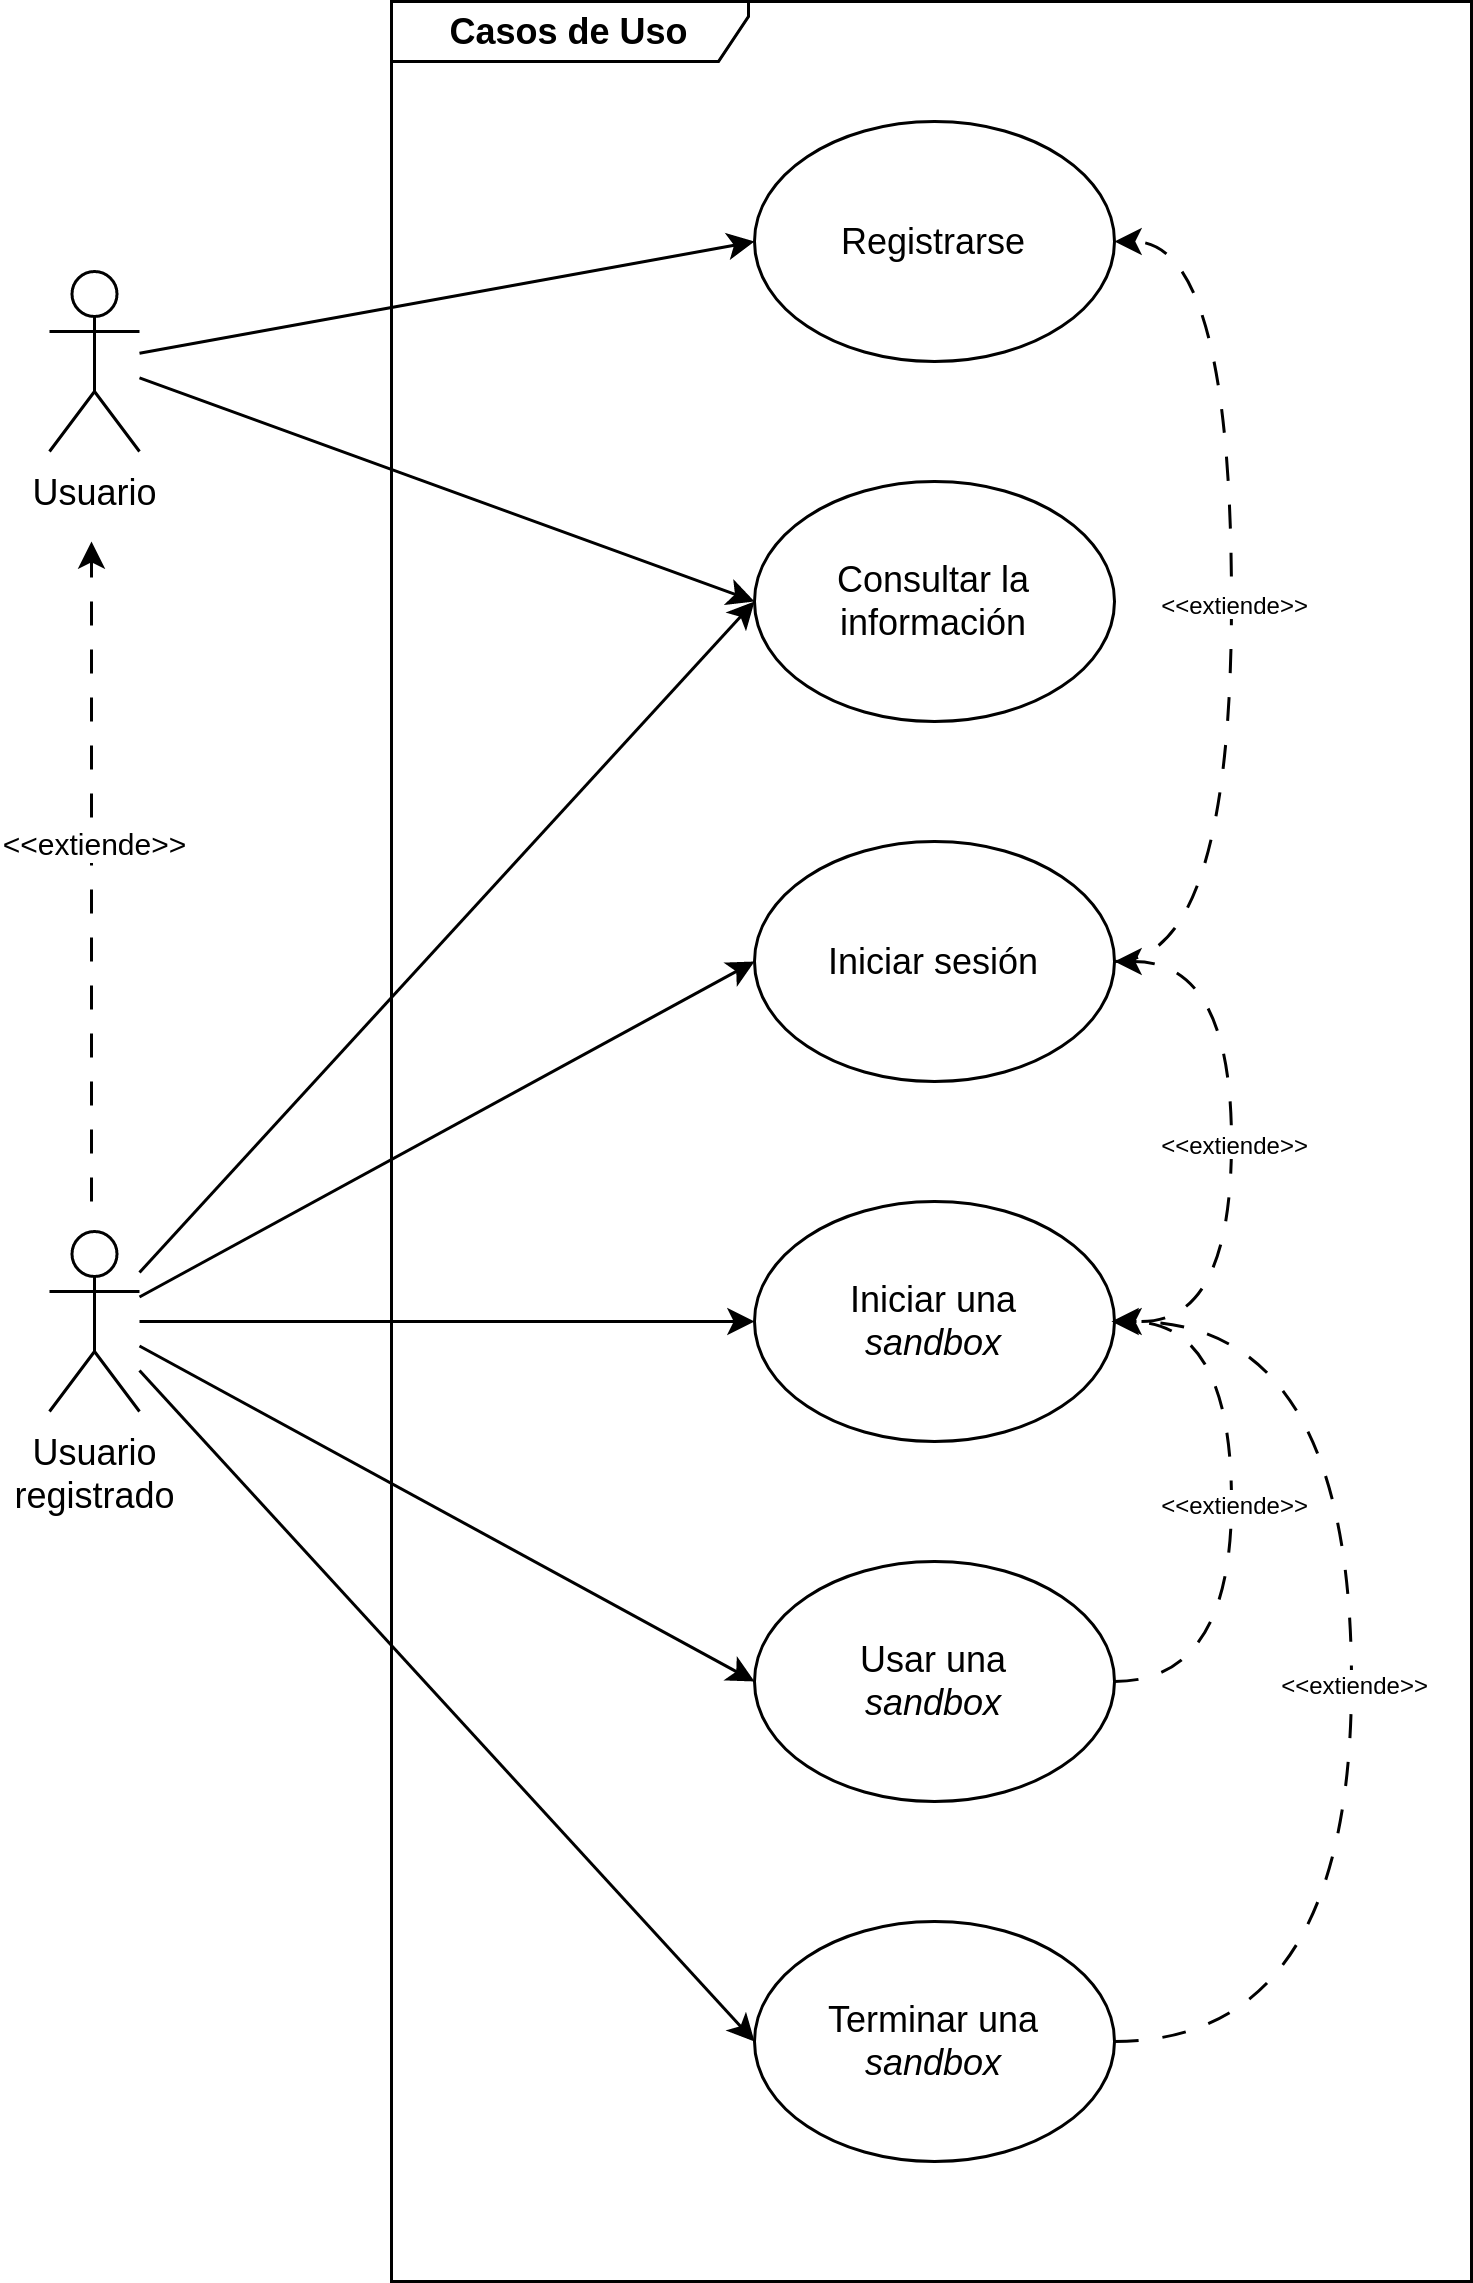
\includegraphics[scale=0.125]{images/Diagramas/Casos de uso.png}

                \caption{Casos de uso}
                \label{fig:casos-uso}
            \end{figure}
            
            \newpage
        
        \subsection{Requisitos funcionales}
            \label{sec:requisitos-funcionales}
            
            Los casos de uso permiten identificar los requisitos funcionales necesarios para satisfacer las necesidades del usuario y asegurarse de que el sistema cumpla con sus objetivos y expectativas. Teniendo eso en cuenta, los casos de uso describen cómo interactúan los usuarios con el sistema y qué acciones o funcionalidades deben estar disponibles en cada situación.
            
            Para este proyecto, se han definido los siguientes requisitos en función de los casos de uso mencionados en el apartado anterior:
            
            \subsubsection{Usuarios}
            
                Requisitos relacionados con la gestión de usuarios y sus datos.
                
                \begin{table}[!htbp]
                    \centering

                    \begin{tabular}{|c|c|}
                        \hline
                        \textbf{RF - 01} & \textbf{Registro de usuarios} \\
                        \hline
                        \multicolumn{2}{|p{15cm}|}{
                            El sistema debe permitir que los usuarios se registren y creen una cuenta en la plataforma para poder usar los laboratorios de pruebas.
                        } \\
                        \hline
                        \multicolumn{2}{|p{15cm}|}{
                            \begin{itemize}
                                \item Nombre de usuario.
                                \item Dirección de correo electrónico.
                                \item Contraseña.
                            \end{itemize}
                            } \\
                        \hline
                    \end{tabular}

                    \label{tab:RF01}
                \end{table}
                
                \begin{table}[!htbp]
                    \centering

                    \begin{tabular}{|c|c|}
                        \hline
                        \textbf{RF - 02} & \textbf{Inicio de sesión} \\
                        \hline
                        \multicolumn{2}{|p{15cm}|}{
                            El sistema debe permitir que los usuarios registrados puedan iniciar sesión para poder acceder al uso de los laboratorios de pruebas.
                        } \\
                        \hline
                    \end{tabular}

                    \label{tab:RF02}
                \end{table}
                
                \begin{table}[!htbp]
                    \centering

                    \begin{tabular}{|c|c|}
                        \hline
                        \textbf{RF - 03} & \textbf{Validación de los datos de registro} \\
                        \hline
                        \multicolumn{2}{|p{15cm}|}{
                            El sistema debe comprobar que los datos de registro de un usuario sean válidos.
                        } \\
                        \hline
                        \multicolumn{2}{|p{15cm}|}{
                            \begin{itemize}
                                \item No se registró un usuario con el mismo nombre de usuario ni correo electrónico.
                                \item Si alguno de los datos no es válido (error), se informará al usuario.
                            \end{itemize}
                            } \\
                        \hline
                    \end{tabular}

                    \label{tab:RF03}
                \end{table}
            
            \subsubsection{Contenido}
            
                Requisitos relacionados con la gestión de contenido y sus características.
                
                \begin{table}[!htbp]
                    \centering

                    \begin{tabular}{|c|c|}
                        \hline
                        \textbf{RF - 04} & \textbf{Consulta de contenido} \\
                        \hline
                        \multicolumn{2}{|p{15cm}|}{
                            El sistema debe proporcionar contenido relevante que permita a los usuarios adquirir los conocimientos necesarios para realizar las pruebas.
                        } \\
                        \hline
                    \end{tabular}

                    \label{tab:RF04}
                \end{table}
                
                \newpage
            
            \subsubsection{Laboratorios de pruebas}
            
                Requisitos relacionados con la gestión de los entornos virtualizados.
                
                \begin{table}[!htbp]
                    \centering

                    \begin{tabular}{|c|c|}
                        \hline
                        \textbf{RF - 05} & \textbf{Inicio de laboratorios de pruebas} \\
                        \hline
                        \multicolumn{2}{|p{15cm}|}{
                            El sistema debe permitir que los usuarios seleccionen e inicien un laboratorio de pruebas que deseen realizar.
                        } \\
                        \hline
                        \multicolumn{2}{|p{15cm}|}{
                            \begin{itemize}
                                \item Si no es posible iniciar un laboratorio (error), se informará al usuario.
                            \end{itemize}
                            } \\
                        \hline
                    \end{tabular}

                    \label{tab:RF05}
                \end{table}
                
                \begin{table}[!htbp]
                    \centering

                    \begin{tabular}{|c|c|}
                        \hline
                        \textbf{RF - 06} & \textbf{Tiempo de vida de los laboratorios de pruebas} \\
                        \hline
                        \multicolumn{2}{|p{15cm}|}{
                            El sistema debe destruir automáticamente un laboratorio iniciado una vez que se haya superado un tiempo de vida definido.
                        } \\
                        \hline
                        \multicolumn{2}{|p{15cm}|}{
                            \begin{itemize}
                                \item Definir un tiempo de vida fijo para los laboratorios de pruebas.
                            \end{itemize}
                            } \\
                        \hline
                    \end{tabular}

                    \label{tab:RF06}
                \end{table}
                
                \begin{table}[!htbp]
                    \centering

                    \begin{tabular}{|c|c|}
                        \hline
                        \textbf{RF - 07} & \textbf{Número máximo de laboratorios de pruebas} \\
                        \hline
                        \multicolumn{2}{|p{15cm}|}{
                            El sistema no debe permitir el inicio de infinitos laboratorios por parte de un usuario.
                        } \\
                        \hline
                        \multicolumn{2}{|p{15cm}|}{
                            \begin{itemize}
                                \item Un usuario solo podrá tener activo un laboratorio a la vez.
                            \end{itemize}
                            } \\
                        \hline
                    \end{tabular}

                    \label{tab:RF07}
                \end{table}
                
                \begin{table}[!htbp]
                    \centering

                    \begin{tabular}{|c|c|}
                        \hline
                        \textbf{RF - 08} & \textbf{Uso de un laboratorio de pruebas iniciado} \\
                        \hline
                        \multicolumn{2}{|p{15cm}|}{
                            El sistema debe permitir que los usuarios puedan conectarse a un laboratorio una vez este se haya iniciado.
                        } \\
                        \hline
                        \multicolumn{2}{|p{15cm}|}{
                            \begin{itemize}
                                \item Proporcionar los datos de conexión a un laboratorio al usuario.
                                \item La conexión se realizará por el propio usuario a través de SSH.
                            \end{itemize}
                            } \\
                        \hline
                    \end{tabular}

                    \label{tab:RF08}
                \end{table}
                
                \begin{table}[!htbp]
                    \centering

                    \begin{tabular}{|c|c|}
                        \hline
                        \textbf{RF - 09} & \textbf{Detención de laboratorios de pruebas} \\
                        \hline
                        \multicolumn{2}{|p{15cm}|}{
                            El sistema debe permitir que los usuarios puedan apagar un laboratorio de pruebas, lo que equivale a destruirla manualmente (en lugar de esperar a que se cumpla su tiempo de vida).
                        } \\
                        \hline
                        \multicolumn{2}{|p{15cm}|}{
                            \begin{itemize}
                                \item Si no es posible destruir un laboratorio (error), se informará al usuario.
                                \item Un administrador podrá acceder a registros de uso de los laboratorios.
                            \end{itemize}
                            } \\
                        \hline
                    \end{tabular}

                    \label{tab:RF09}
                \end{table}
                
                \newpage
        
        \subsection{Requisitos no funcionales}
            \label{sec:requisitos-nofuncionales}
            
            Por otro lado, los requisitos no funcionales describen las cualidades o atributos que debe tener un sistema, enfocándose en cómo hace el sistema lo que hace; es decir, cómo se comporta en términos de calidad.
            
            Para este proyecto, se han definido los siguientes requisitos en función de los requisitos mencionados en la sección anterior, así como los objetivos de la plataforma:
            
            \begin{table}[!htbp]
                \centering

                \begin{tabular}{|c|c|}
                    \hline
                    \textbf{RNF - 01} & \textbf{Privacidad de los datos} \\
                    \hline
                    \multicolumn{2}{|p{15cm}|}{
                        El sistema debe garantizar la seguridad y privacidad de los datos de los usuarios.
                    } \\
                    \hline
                    \multicolumn{2}{|p{15cm}|}{
                        \begin{itemize}
                            \item Aplicar una política de cifrado para las contraseñas.
                        \end{itemize}
                        } \\
                    \hline
                \end{tabular}

                \label{tab:RNF1}
            \end{table}
            
            \begin{table}[!htbp]
                \centering

                \begin{tabular}{|c|c|}
                    \hline
                    \textbf{RNF - 02} & \textbf{Aislamiento de los laboratorios de pruebas} \\
                    \hline
                    \multicolumn{2}{|p{15cm}|}{
                        El sistema debe garantizar la seguridad y aislamiento de los laboratorios de prueba de la plataforma.
                    } \\
                    \hline
                    \multicolumn{2}{|p{15cm}|}{
                        \begin{itemize}
                            \item Aislar completamente los laboratorios sin afectar al resto de la plataforma.
                        \end{itemize}
                        } \\
                    \hline
                \end{tabular}

                \label{tab:RNF2}
            \end{table}
            
            \begin{table}[!htbp]
                \centering

                \begin{tabular}{|c|c|}
                    \hline
                    \textbf{RNF - 03} & \textbf{Seguridad de la plataforma} \\
                    \hline
                    \multicolumn{2}{|p{15cm}|}{
                        El sistema debe implementar medidas de seguridad para prevenir ataques externos o internos a la plataforma.
                    } \\
                    \hline
                    \multicolumn{2}{|p{15cm}|}{
                        \begin{itemize}
                            \item Medidas de autenticación y autorización para garantizar el acceso solo a usuarios autorizados.
                        \end{itemize}
                        } \\
                    \hline
                \end{tabular}

                \label{tab:RNF3}
            \end{table}
            
            \begin{table}[!htbp]
                \centering

                \begin{tabular}{|c|c|}
                    \hline
                    \textbf{RNF - 04} & \textbf{Accesibilidad} \\
                    \hline
                    \multicolumn{2}{|p{15cm}|}{
                        La plataforma debe ser accesible para cualquier usuario, independientemente de su nivel de experiencia en ciberseguridad.
                    } \\
                    \hline
                    \multicolumn{2}{|p{15cm}|}{
                        \begin{itemize}
                            \item Contenido claro, accesible y bien estructurado.
                        \end{itemize}
                        } \\
                    \hline
                \end{tabular}

                \label{tab:RNF4}
            \end{table}
            
            \begin{table}[!htbp]
                \centering

                \begin{tabular}{|c|c|}
                    \hline
                    \textbf{RNF - 05} & \textbf{Usabilidad} \\
                    \hline
                    \multicolumn{2}{|p{15cm}|}{
                        La plataforma debe ser fácil de usar y accesible para cualquier usuario, independientemente de su nivel de experiencia en ciberseguridad.
                    } \\
                    \hline
                    \multicolumn{2}{|p{15cm}|}{
                        \begin{itemize}
                            \item Interfaz de usuario intuitiva, clara y organizada.
                        \end{itemize}
                        } \\
                    \hline
                \end{tabular}

                \label{tab:RNF5}
            \end{table}
            
            \begin{table}[H]
                \centering

                \begin{tabular}{|c|c|}
                    \hline
                    \textbf{RNF - 06} & \textbf{Extensibilidad} \\
                    \hline
                    \multicolumn{2}{|p{15cm}|}{
                        La plataforma debe ser fácilmente extensible, permitiendo la futura integración de más contenido y laboratorios de pruebas.
                    } \\
                    \hline
                    \multicolumn{2}{|p{15cm}|}{
                        \begin{itemize}
                            \item Definir y documentar claramente cómo añadir contenido y laboratorios.
                        \end{itemize}
                        } \\
                    \hline
                \end{tabular}

                \label{tab:RNF6}
            \end{table}
            
            \newpage
    
    \section{Arquitectura}
        \label{sec:arquitectura}
        
        \begin{figure}[h]
            \centering

            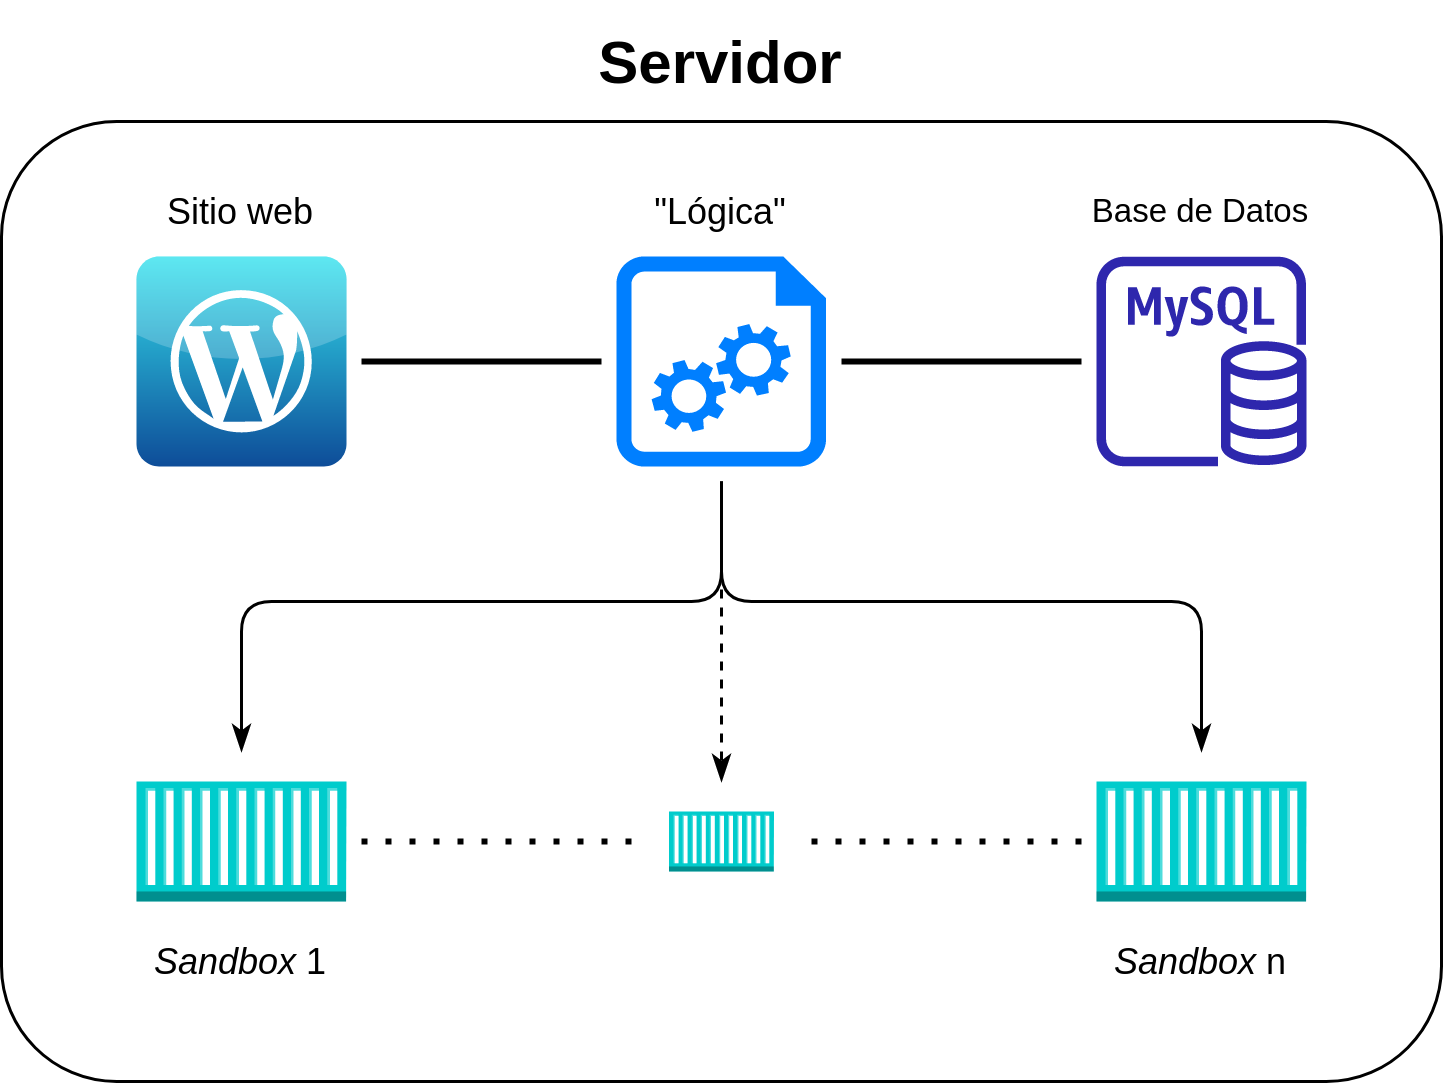
\includegraphics[scale=0.20]{images/Diagramas/Arquitectura.png}

            \caption{Arquitectura}
            \label{fig:arquitectura}
        \end{figure}

        Los componentes de la plataforma podrían dividirse en 4 partes fundamentales: el front-end, el back-end, la base de datos y los contenedores Docker (laboratorios). Todos estos están desplegados en un servidor que utiliza LAMP.

        \subsection{\textit{Front-end}: WordPress}

            El front-end es la parte de la plataforma que interactúa con el usuario; en este caso, se ha desarrollado una aplicación web que permite al usuario acceder a la plataforma y realizar las acciones que se describen en la sección \ref{sec:casos-uso}.
            
            Esta plataforma web se ha desarrollado utilizando el gestor de contenidos WordPress, ya que permite crear sitios web de forma rápida y sencilla, sin necesidad de tener conocimientos avanzados de programación. Además, cuenta con una gran comunidad de desarrolladores que crean y mantienen plugins y temas para extender las funcionalidades de la plataforma.

            Se ha usado un tema hijo del tema \textit{Divi}, que permite crear sitios web de forma visual, sin necesidad de escribir código. Este tema hijo se ha usado para personalizar el tema \textit{Divi} y adaptarlo a las necesidades de la plataforma. Se seleccionó este tema porque es muy conocido y está muy bien valorado en la comunidad.

        \subsection{\textit{Back-end}: \texttt{functions.php}}
        
            El back-end es la parte de la plataforma que se encarga de procesar las peticiones del usuario y de gestionar los recursos de la plataforma; en este proyecto, se encarga de gestionar las peticiones del usuario y de comunicarse con la base de datos y los contenedores Docker.
            
            Se ha usado el fichero \texttt{functions.php} de WordPress para implementar el back-end de la plataforma, ya que permite extender las funcionalidades de un sitio web de WordPress de forma sencilla.
            
            Este fichero se ejecuta en cada petición que se realiza a la plataforma, lo que permite interactuar con la página cada vez que un usuario interactúa con ella.

            \subsubsection{\textit{Back-end}: Tareas de Cron}

                Las tareas de cron son tareas que se ejecutan de forma periódica en el servidor. Se ha usado una para comprobar si algún laboratorio de pruebas superó su tiempo de vida (1 hora) y detenerlo de forma automática.
                
                Esta tarea se ha implementado directamente en el servidor, ya que se consideró la opción más rápida y sencilla: se ejecuta cada minuto y destruye aquellos laboratorios que hayan excedido su tiempo de vida, liberando recursos en el sistema y permitiendo un uso de contenedores dinámico.

        \subsection{Base de datos: MySQL}

            La base de datos es la parte de la plataforma que se encarga de almacenar la información de los usuarios y de los laboratorios de pruebas; en este caso, se ha usado para almacenar la información de los usuarios registrados en la plataforma y de los laboratorios de pruebas que han sido creados por dichos usuarios.
            
            Se ha usado MySQL como gestor de base de datos, ya que es un sistema de gestión de bases de datos relacional, de código abierto y muy popular. Además, es compatible con WordPress, por lo que se puede acceder a la base de datos desde el fichero \textit{functions.php}.
        
        \subsection{Contenedores Docker: laboratorios de pruebas}

            Los contenedores Docker son la parte de la plataforma que se encarga de ejecutar los laboratorios de pruebas. En este caso, se ha usado para ejecutar los laboratorios de pruebas que han sido creados por los usuarios.
            
            Se ha usado Docker para ejecutar los laboratorios de pruebas, ya que permite ejecutar aplicaciones en contenedores de software. Estos contenedores son ligeros y portables, por lo que se pueden ejecutar en cualquier máquina que tenga Docker instalado. Además, se pueden crear imágenes de los contenedores, lo que permite crear laboratorios de pruebas personalizados y compartirlos con otros usuarios.

            Por otra parte, los laboratorios son construidos a partir de imágenes contruidas con ficheros \texttt{Dockerfile} locales, por lo que pueden crearse nuevos laboratorios de pruebas de forma rápida y sencilla para extender la plataforma.
            
            \newpage
    
    \section{Modelado de actividades y transiciones}
        \label{sec:modelado-actividades-transiciones}

        Los diagramas mostrados a continuación presentan las actividades que puede realizar un usuario en la plataforma y las transiciones entre dichas actividades.
        
        Estos diagramas se han desarrollado utilizando la herramienta \textit{draw.io}.
        
        \subsection{Tratamiento de usuarios}
        
            \begin{figure}[h]
                \centering

                \begin{subfigure}{0.45\textwidth}
                    \centering
                    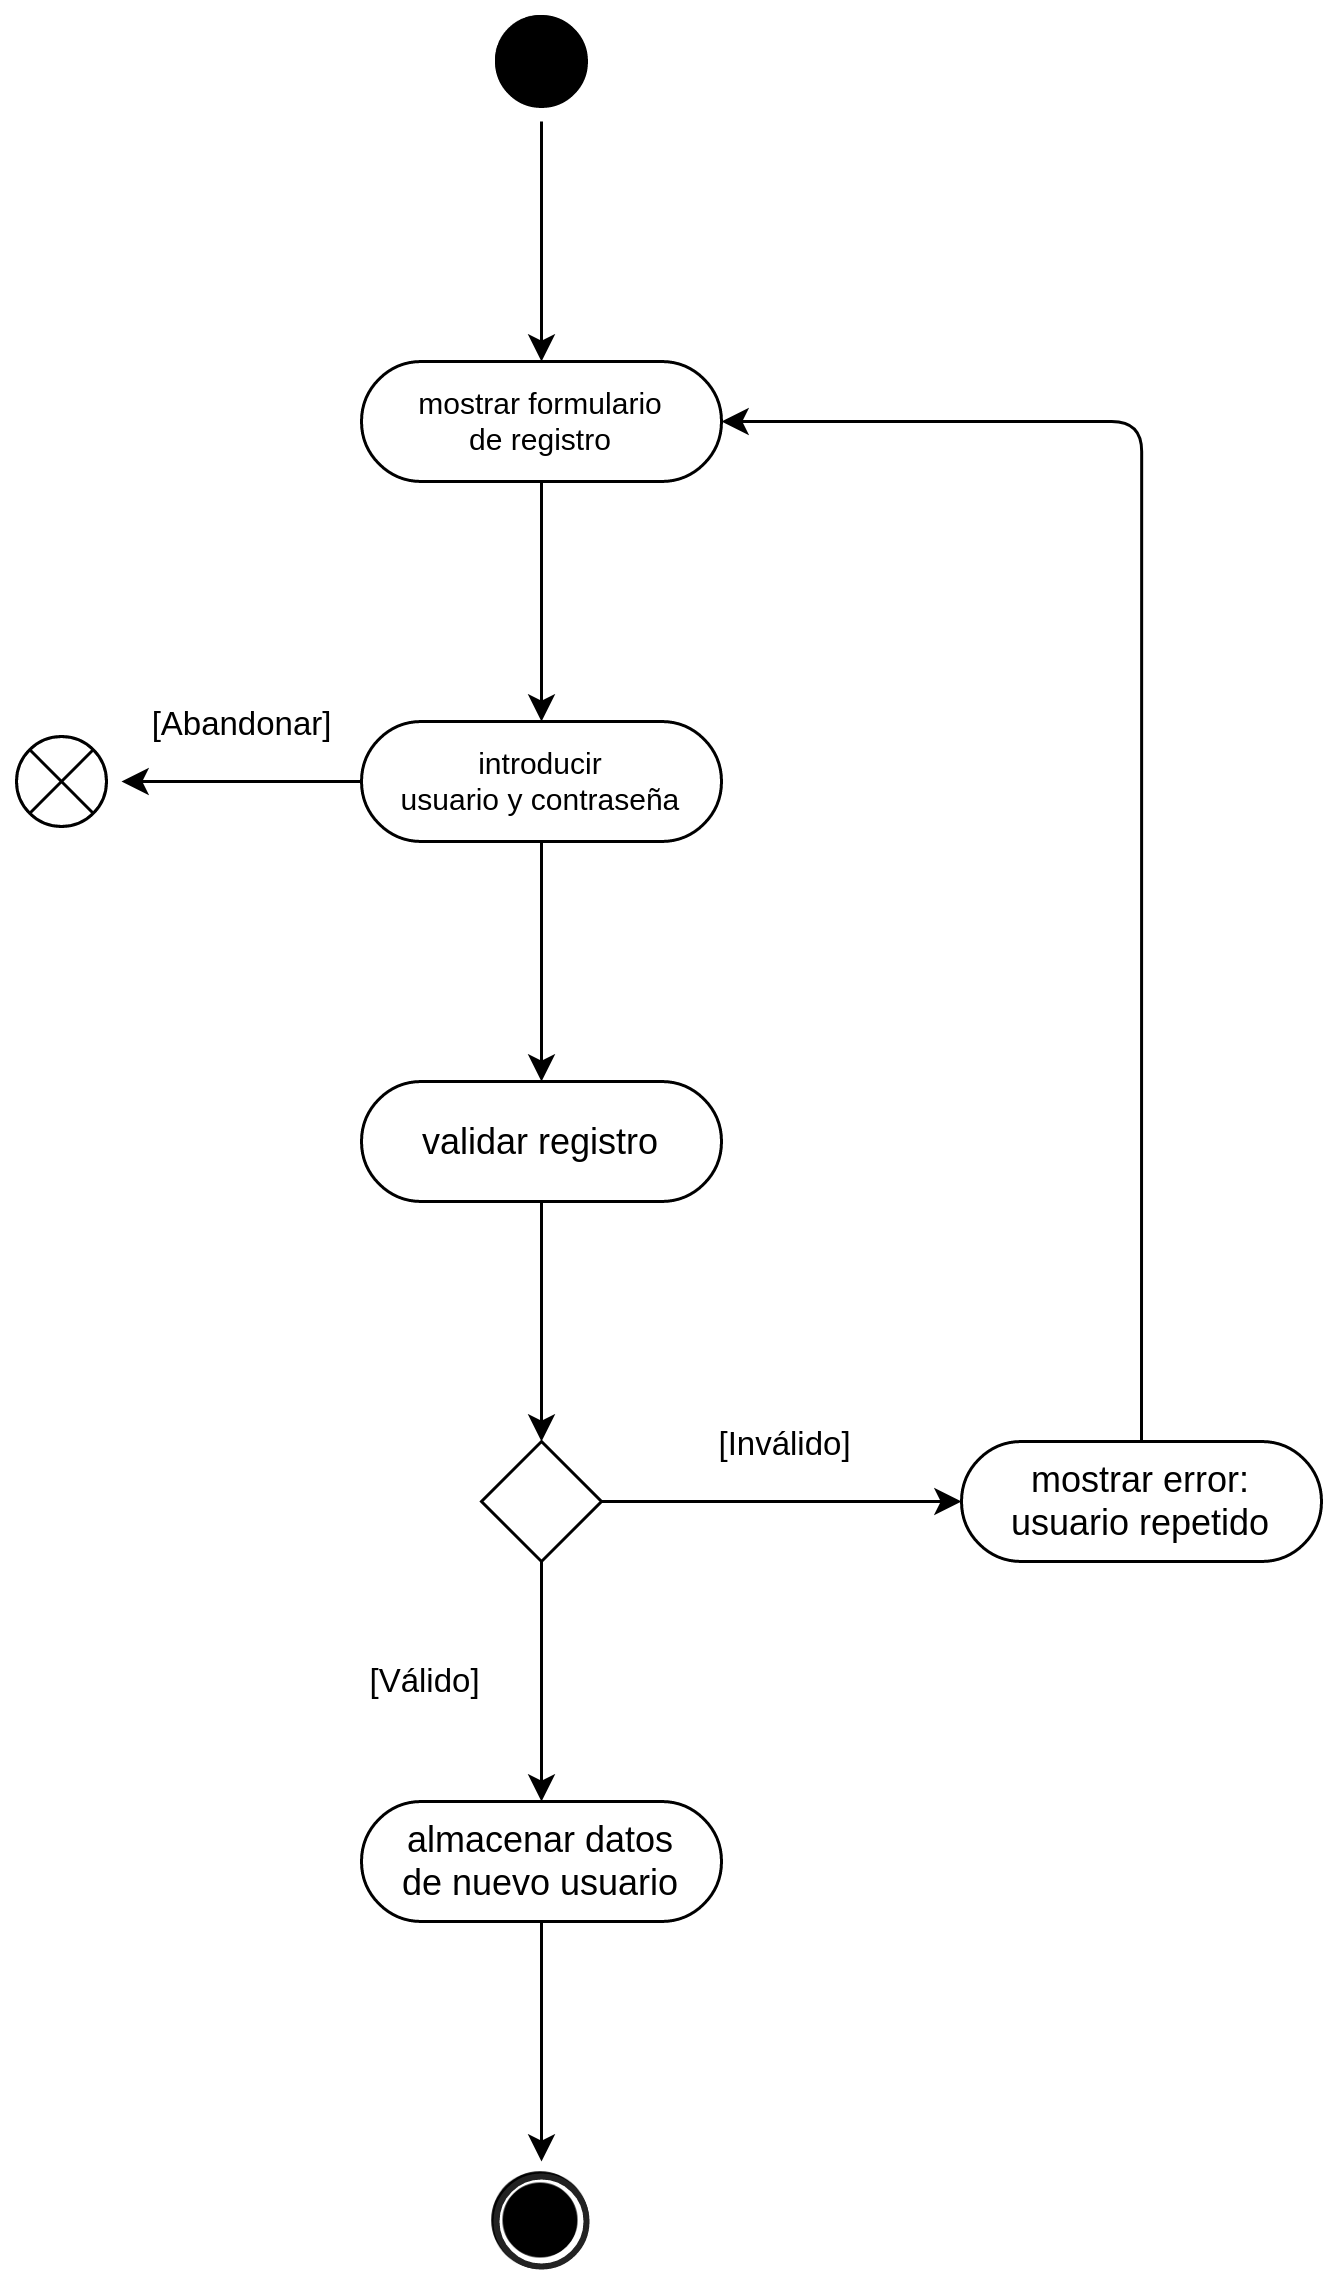
\includegraphics[scale=0.15]{images/Diagramas/Actividades y transiciones 1.png}
                    \caption{Registro de un usuario}
                    \label{fig:registro-usuario}
                \end{subfigure}
                \hfill
                \begin{subfigure}{0.45\textwidth}
                    \centering
                    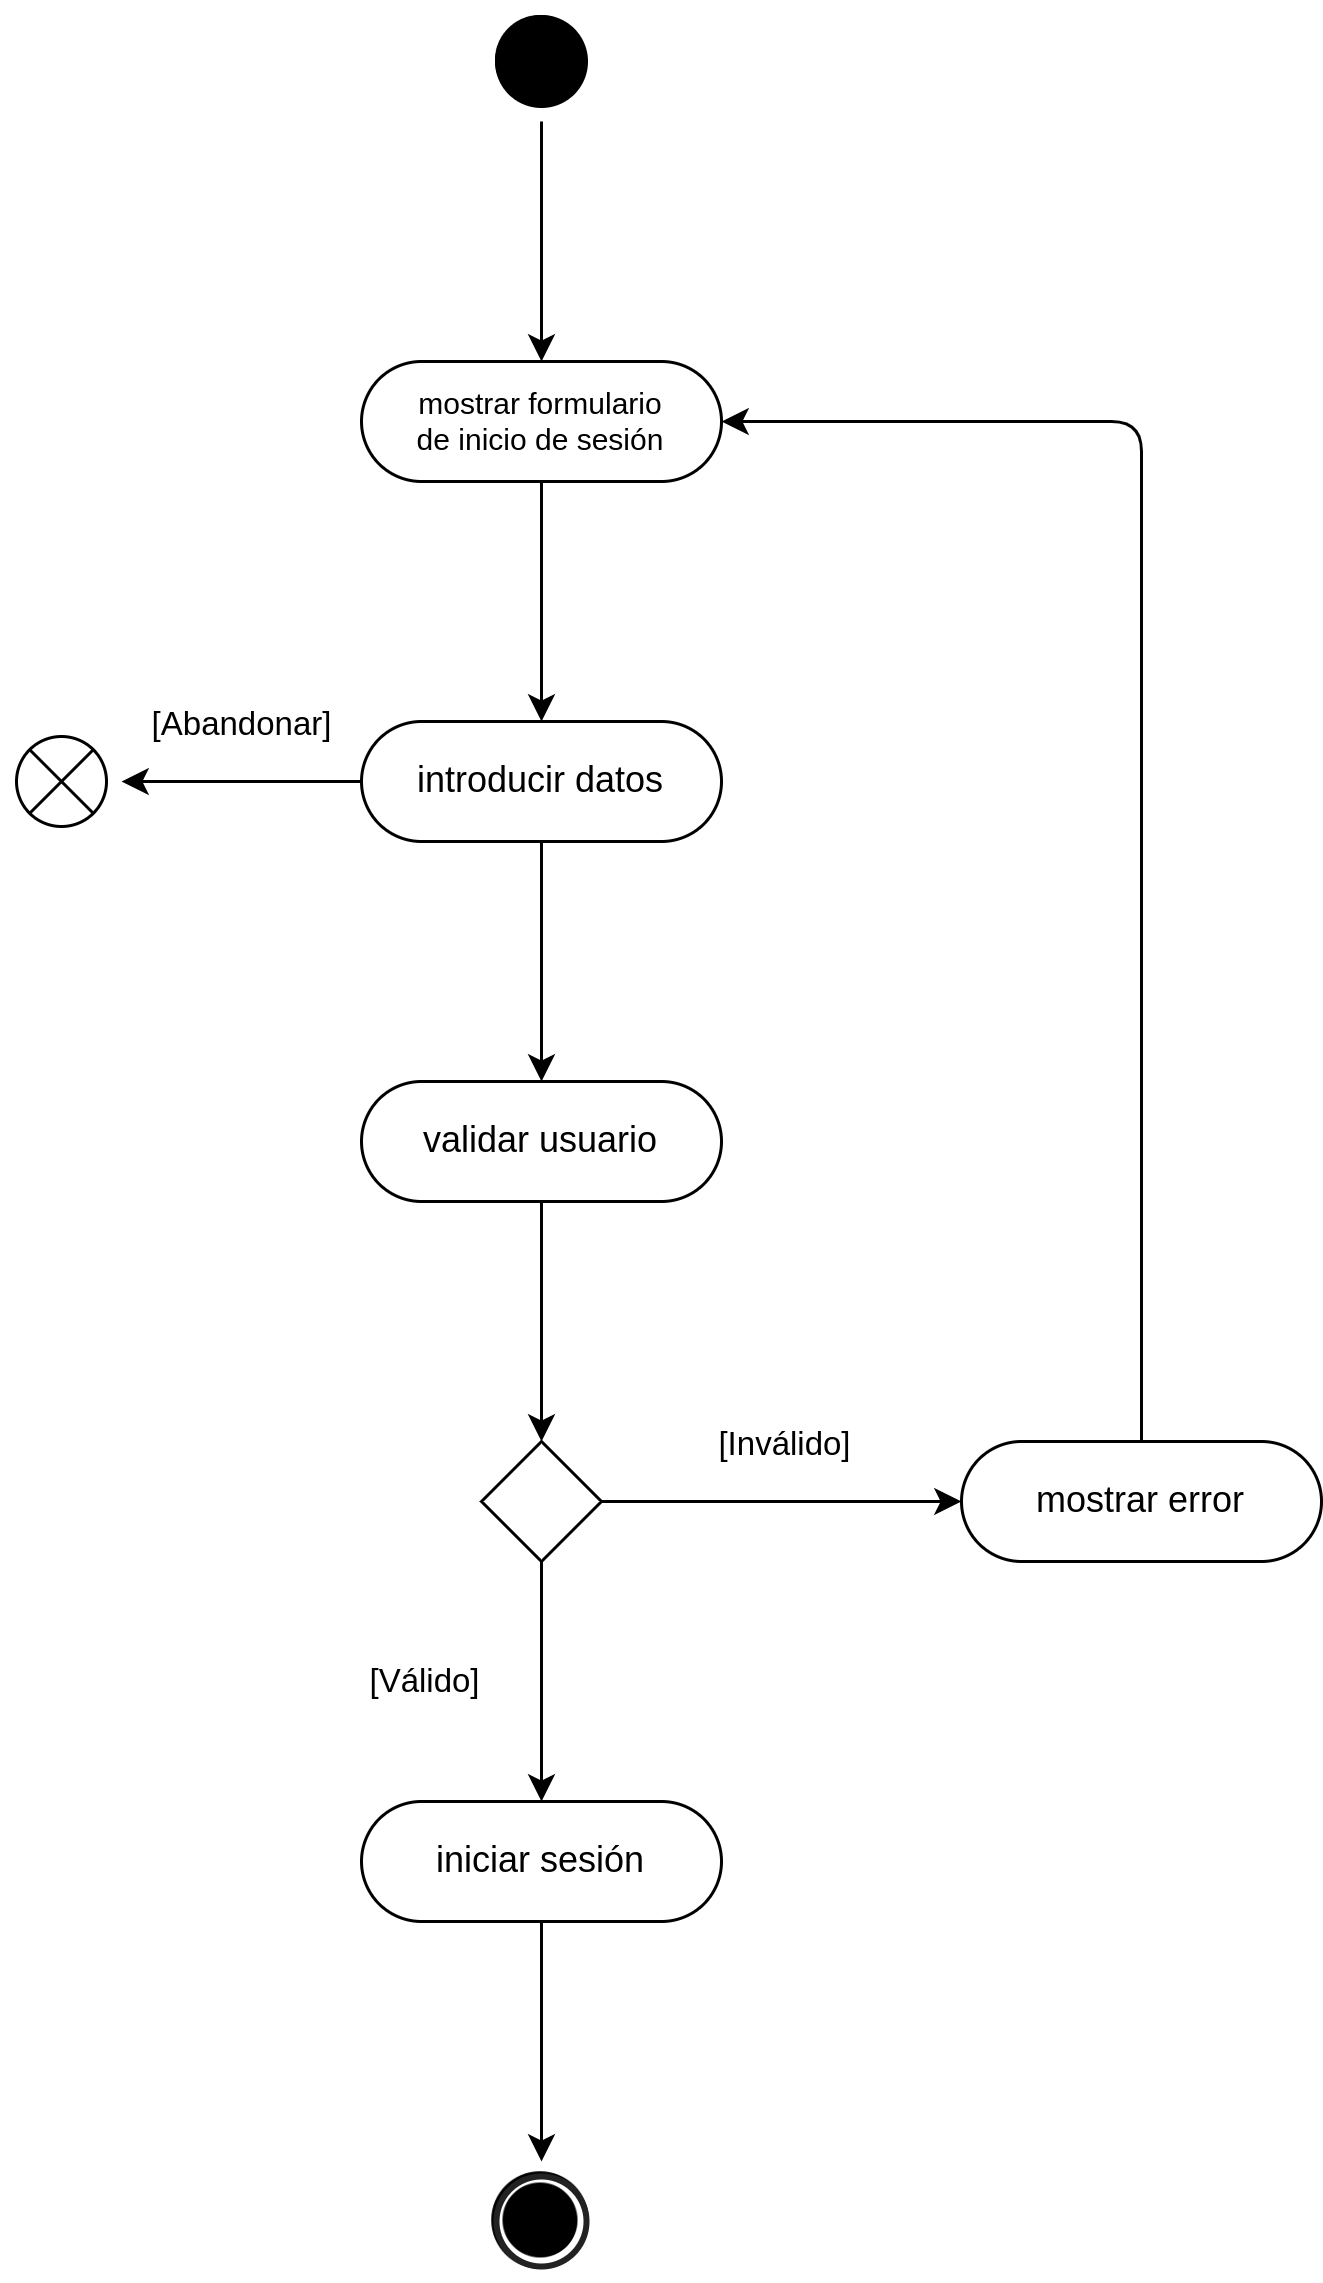
\includegraphics[scale=0.15]{images/Diagramas/Actividades y transiciones 2.png}
                    \caption{Inicio de sesión de un usuario}
                    \label{fig:inicio-usuario}
                \end{subfigure}

                \caption{Modelado de actividades y transiciones}
                \label{fig:tratamiento-usuarios}
            \end{figure}
            
            Los diagramas presentados en esta sección definen la gestión de usuarios que permite el registro e inicio de sesión de los mismos en la plataforma.
            
            El proceso de registro de un usuario mostrará inicialmente un formulario para poder obtener sus datos, debiendo verificar que dichos datos no pertenecen a un usario previamente registrado, puesto que los usuarios deben ser únicos.
            
            El proceso de inicio de sesión de un usuario mostrará un funcionamiento similar al de registro, pero esta vez, para comprobar que el usuario sí ha sido registrado anteriormente.
            
            \newpage
            
        \subsection{Consulta de la documentación}
            \label{sec:consulta-documentacion}
            
            \begin{figure}[h]
                \centering
                
                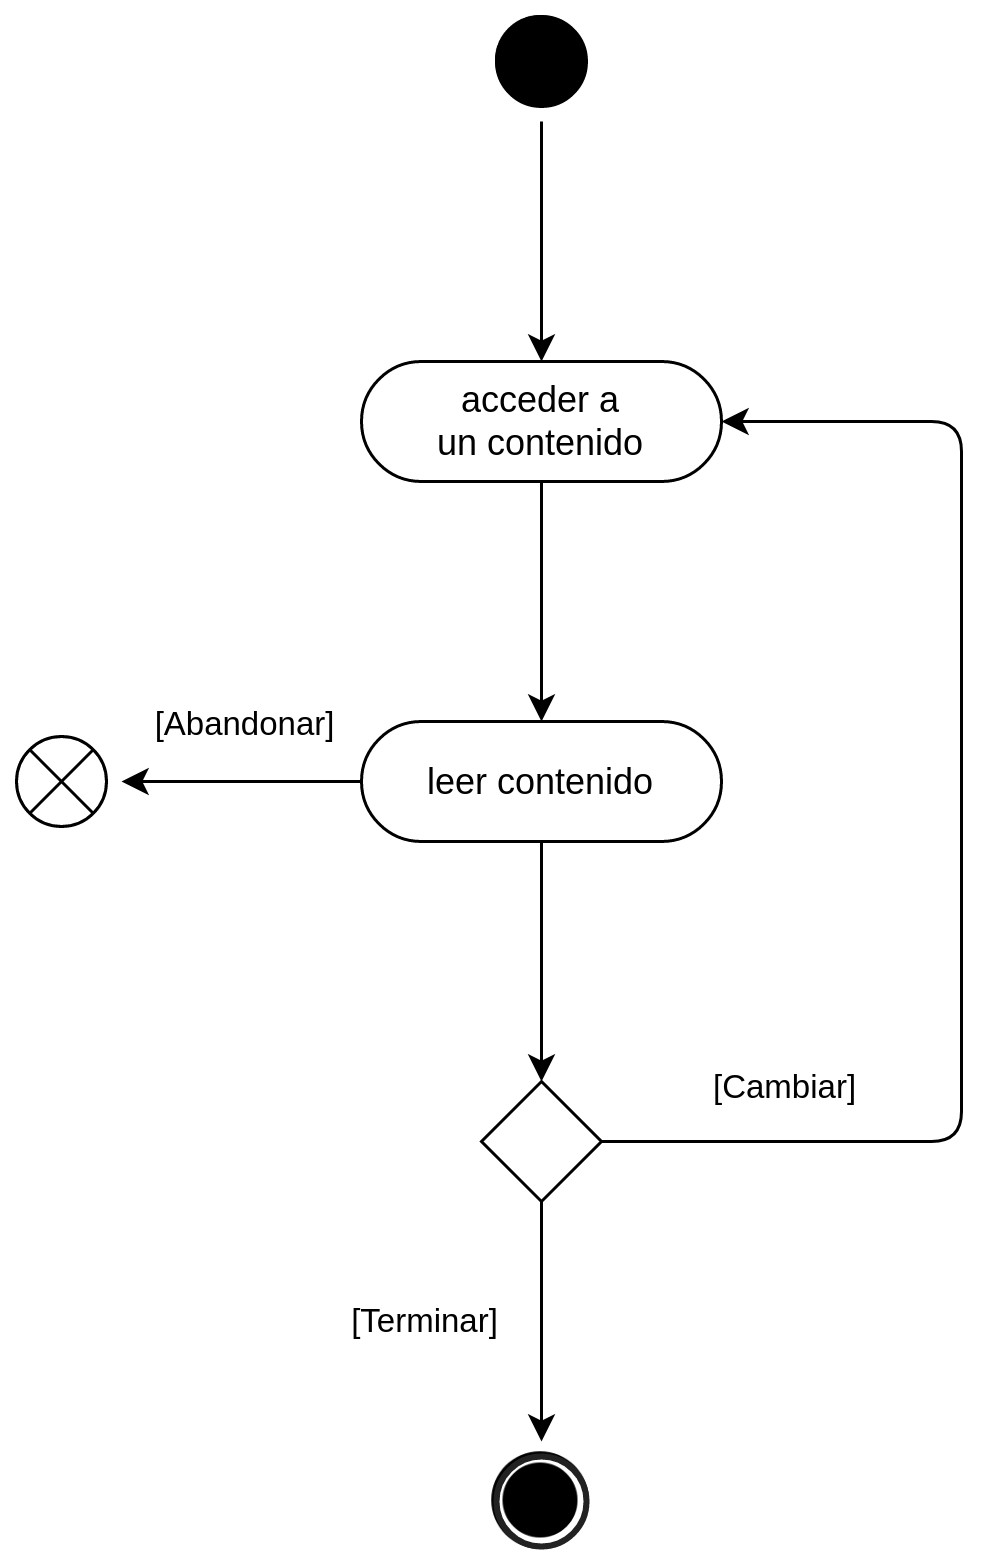
\includegraphics[scale=0.20]{images/Diagramas/Actividades y transiciones 3.png}

                \caption{Consulta de documentación}
                \label{fig:consulta-documentacion}
            \end{figure}
            
            El diagrama presentado en esta sección define el consumo de contenido de la plataforma por parte de un usuario, esté registrado o no, ya que el contenido instructivo de la plataforma se considera público, al contrario que el uso de los laboratorios que requerirá un registro por parte del usuario.
            
            El proceso de consulta de documentación es bastante simple: un usuario puede consumir contenido de forma continua, pero al estar dividido por conceptos, necesitará cambiar de ubicación dentro de la plataforma para poder seguir accediendo a contenido nuevo.
            
            \newpage
            
        \subsection{Tratamiento de laboratorios}
        
            \begin{figure}[h]
                \centering
                
                \begin{subfigure}{0.45\textwidth}
                    \centering
                    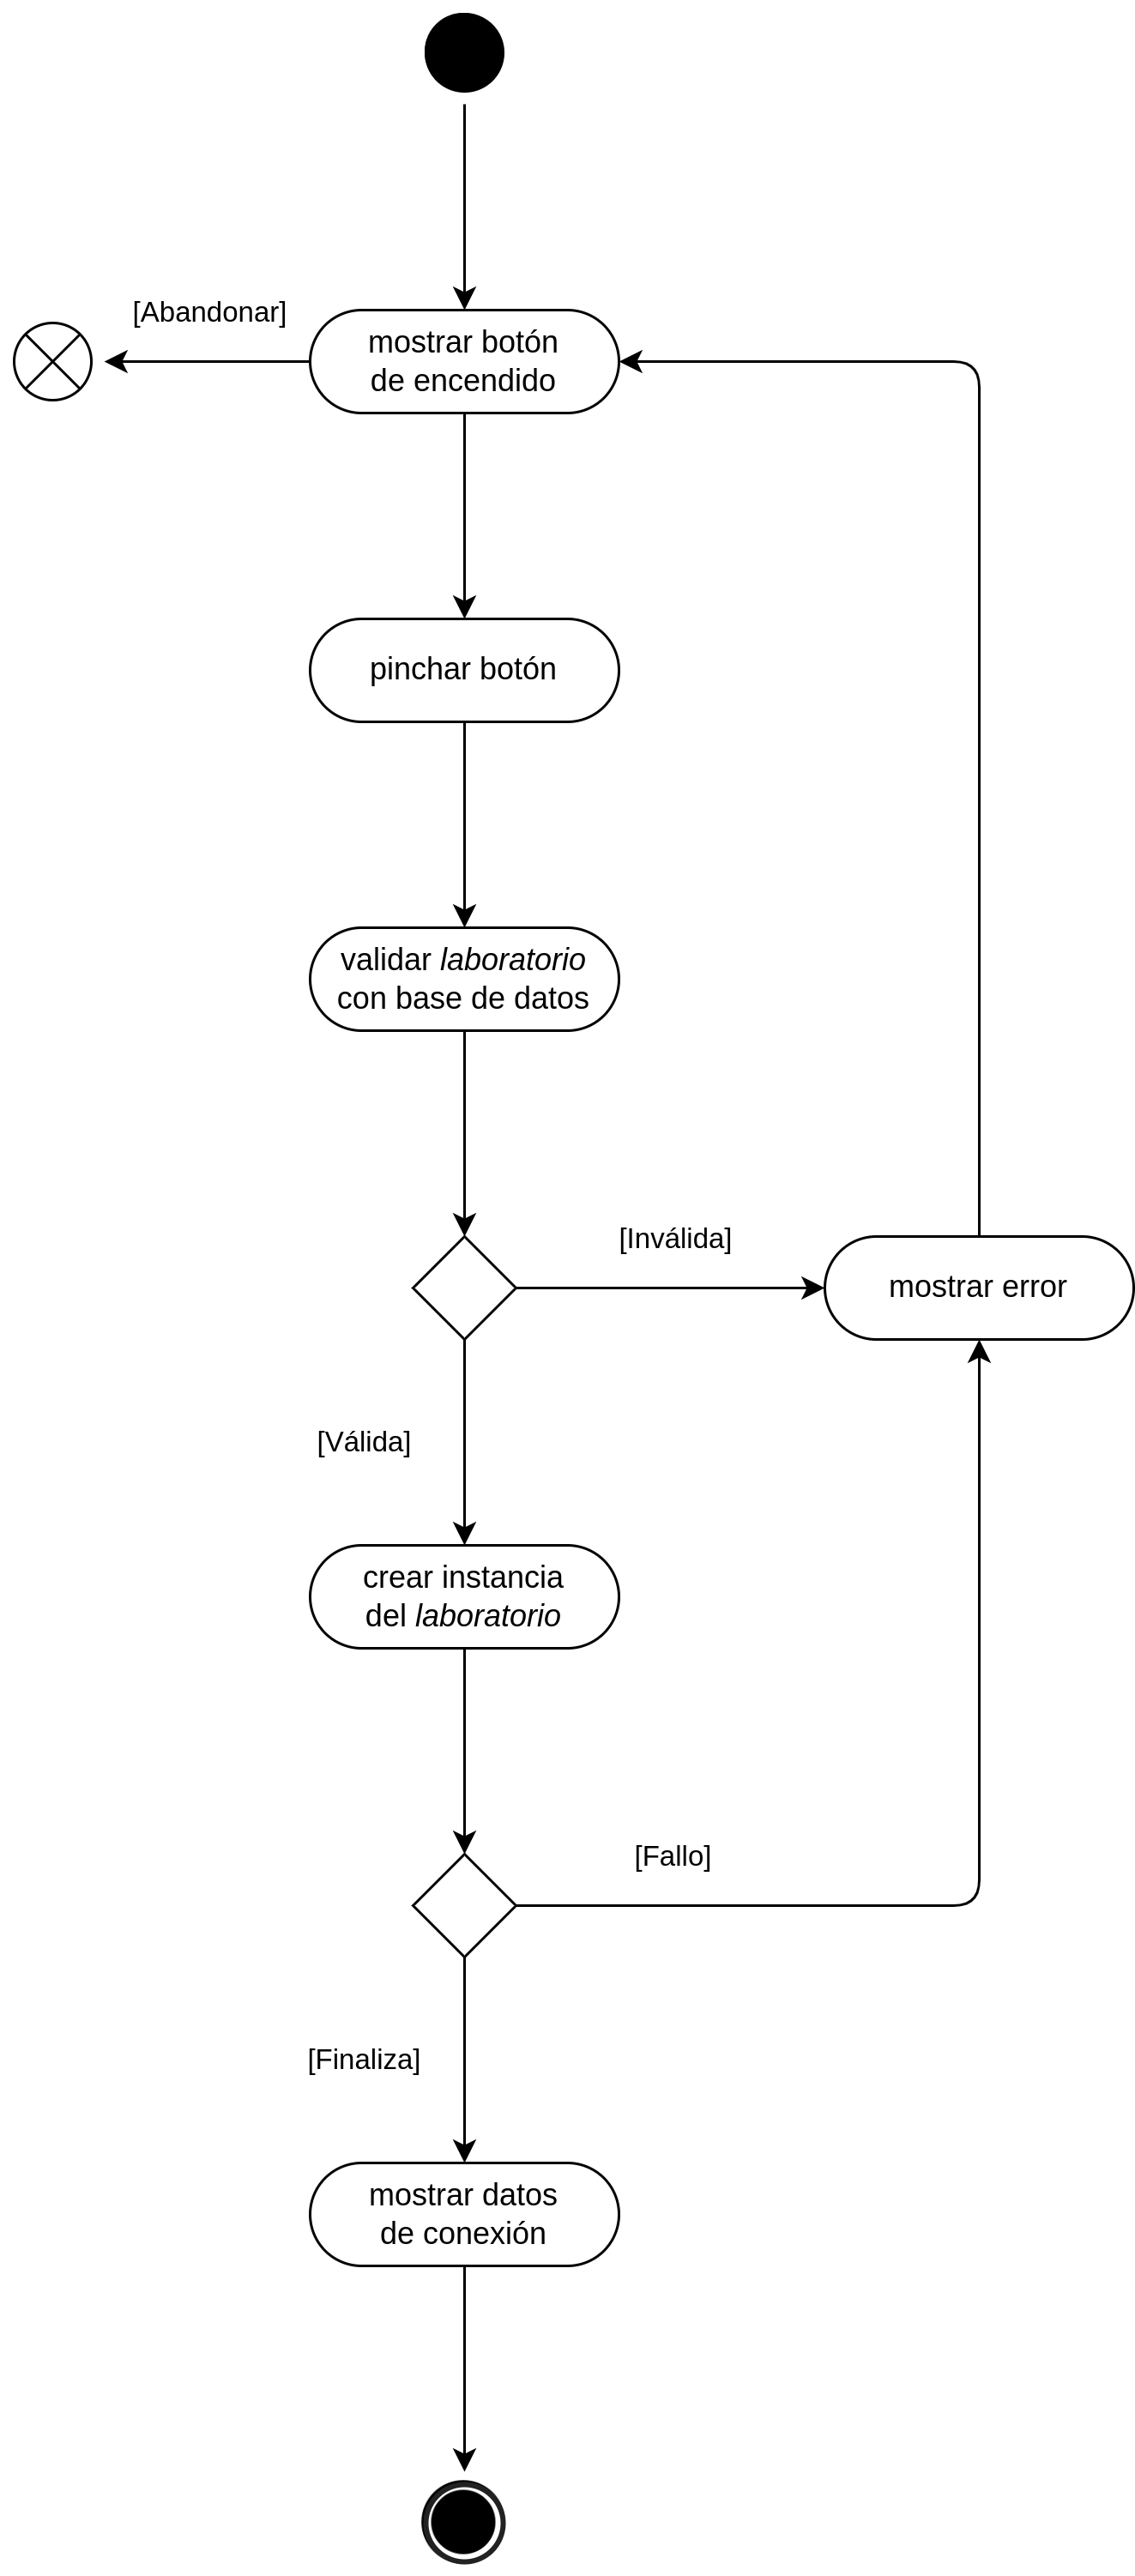
\includegraphics[scale=0.115]{images/Diagramas/Actividades y transiciones 4.png}
                    \caption{Creación de un laboratorio}
                    \label{fig:creacion-laboratorio}
                \end{subfigure}
                \hfill
                \begin{subfigure}{0.45\textwidth}
                    \centering
                    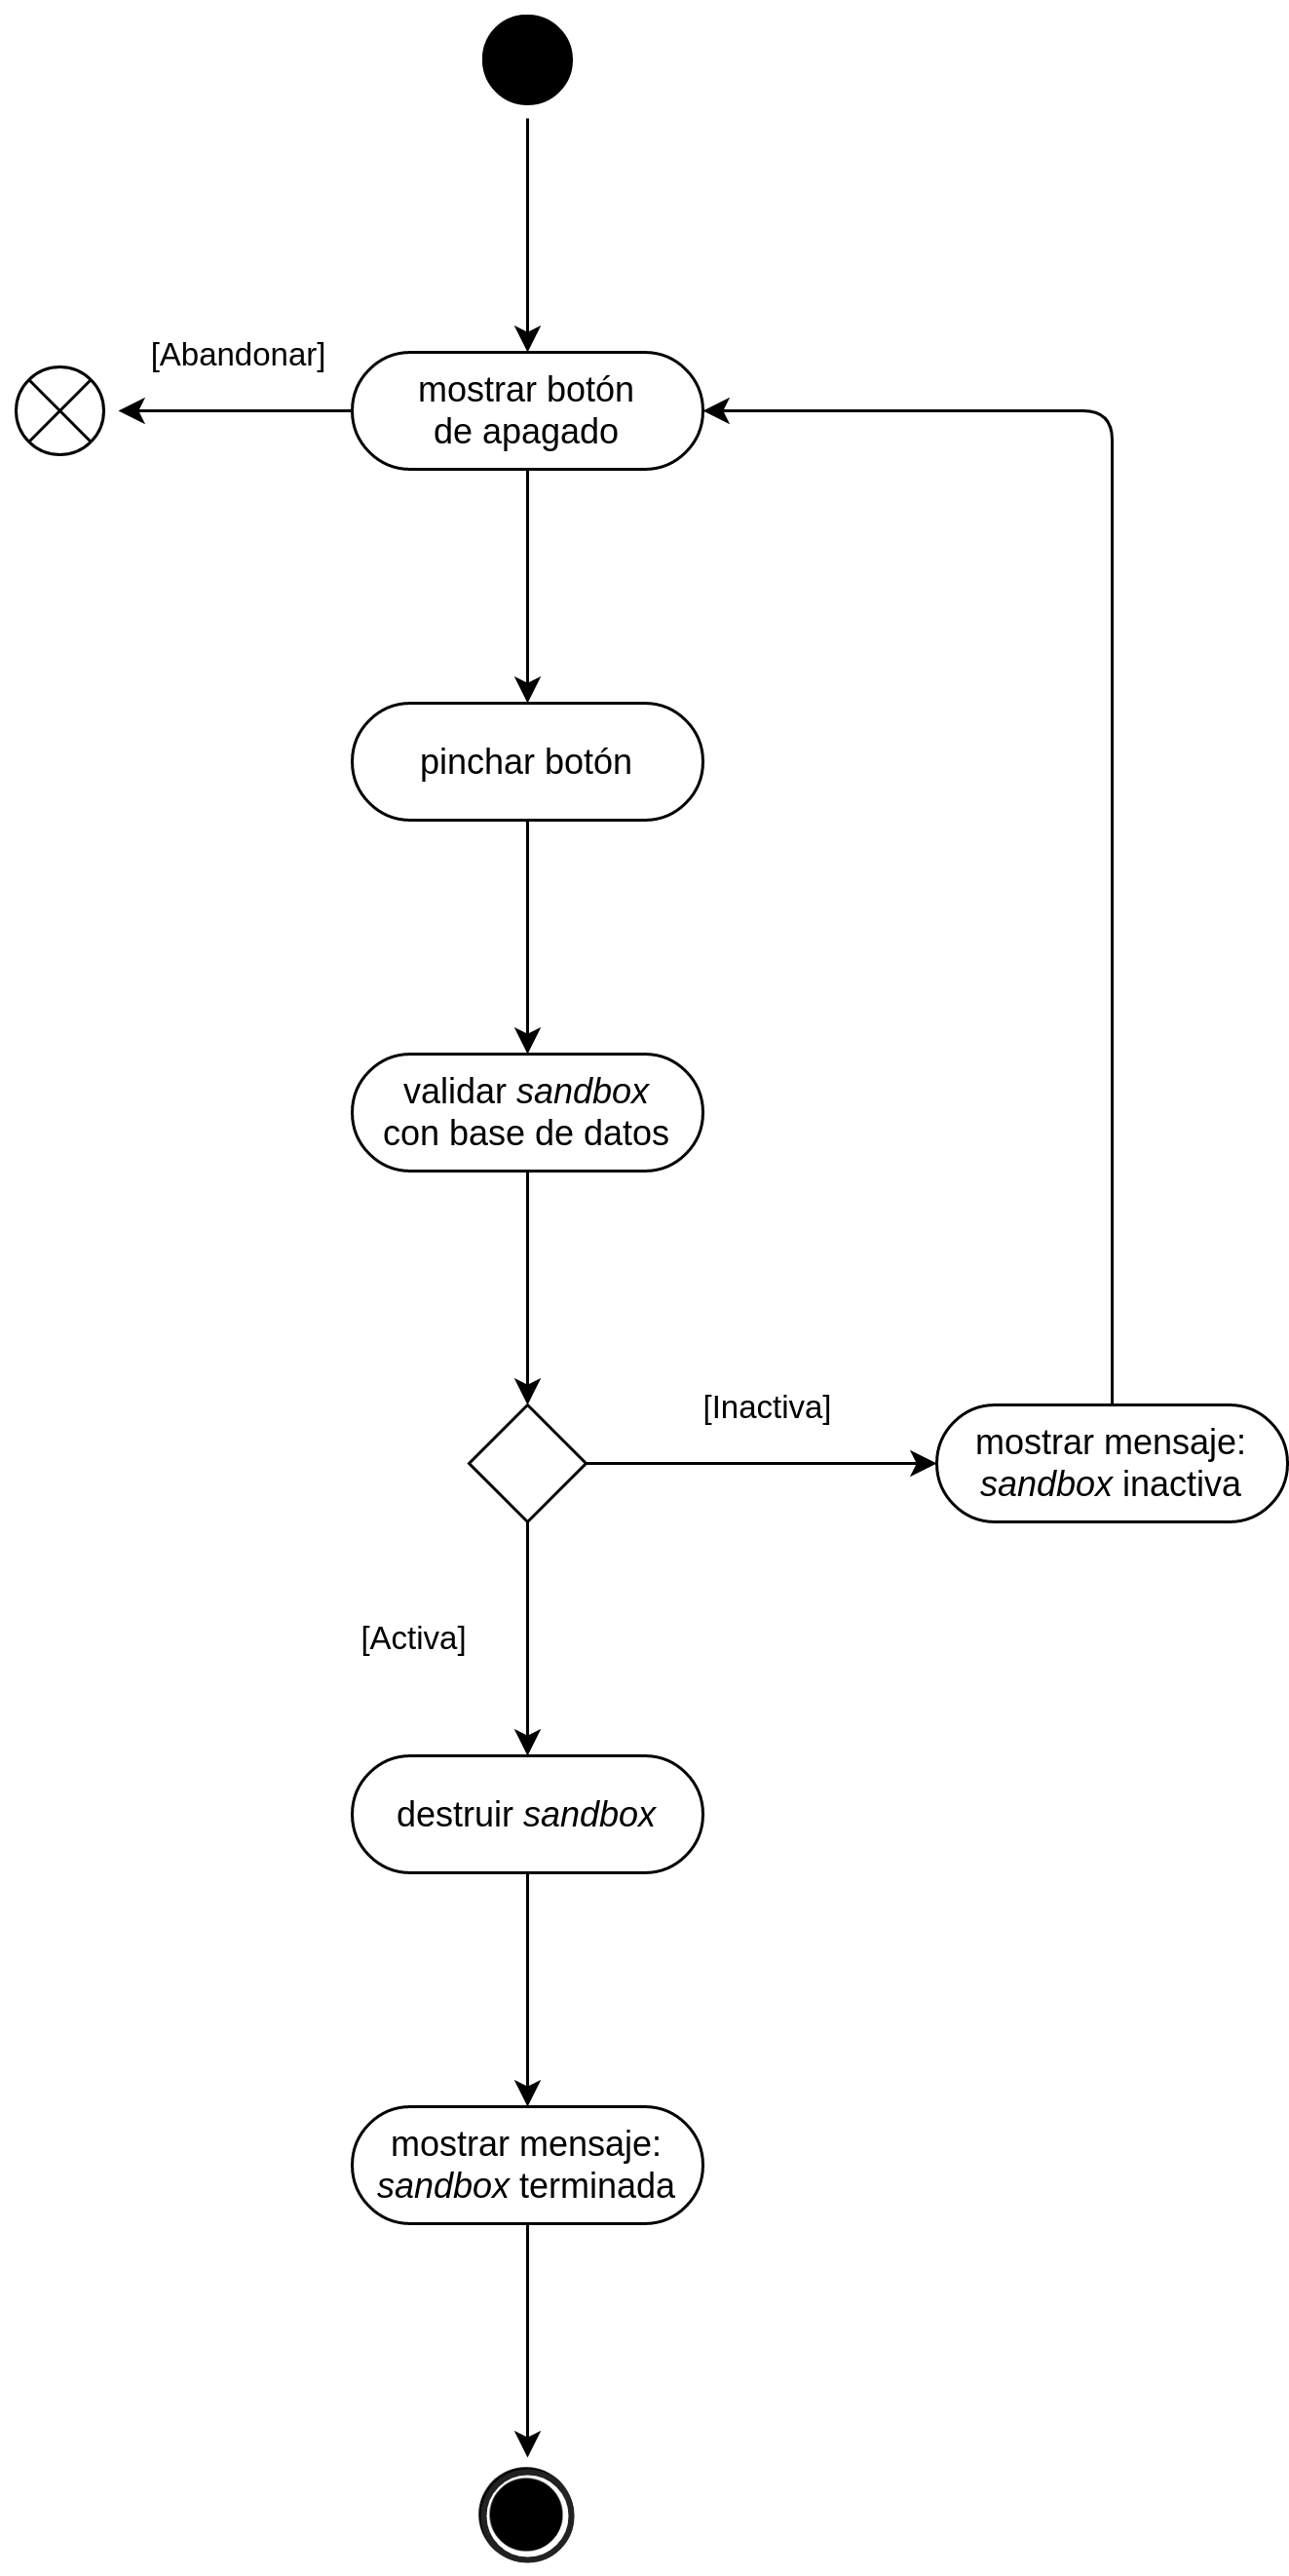
\includegraphics[scale=0.115]{images/Diagramas/Actividades y transiciones 5.png}
                    \caption{Destrucción de un laboratorio}
                    \label{fig:destruccion-laboratorio}
                \end{subfigure}

                \caption{Tratamiento de laboratorios}
                \label{fig:tratamiento-laboratorios}
            \end{figure}
            
            Los diagramas presentados en esta sección definen la gestión de entornos virtualizados de la plataforma.
            
            El proceso de creación de un laboratorio iniciará pulsando un botón, preferiblemente ubicado al final de un contenido instructivo descrito anteriormente en la sección \ref{sec:consulta-documentacion}, debiendo verificar que es posible crear dicho laboratorio.
            
            El proceso de destrucción de un laboratorio seguirá el mismo proceso que el anterior, pero realizará la opción opuesta.

            \newpage

            \begin{figure}[h]
                \centering

                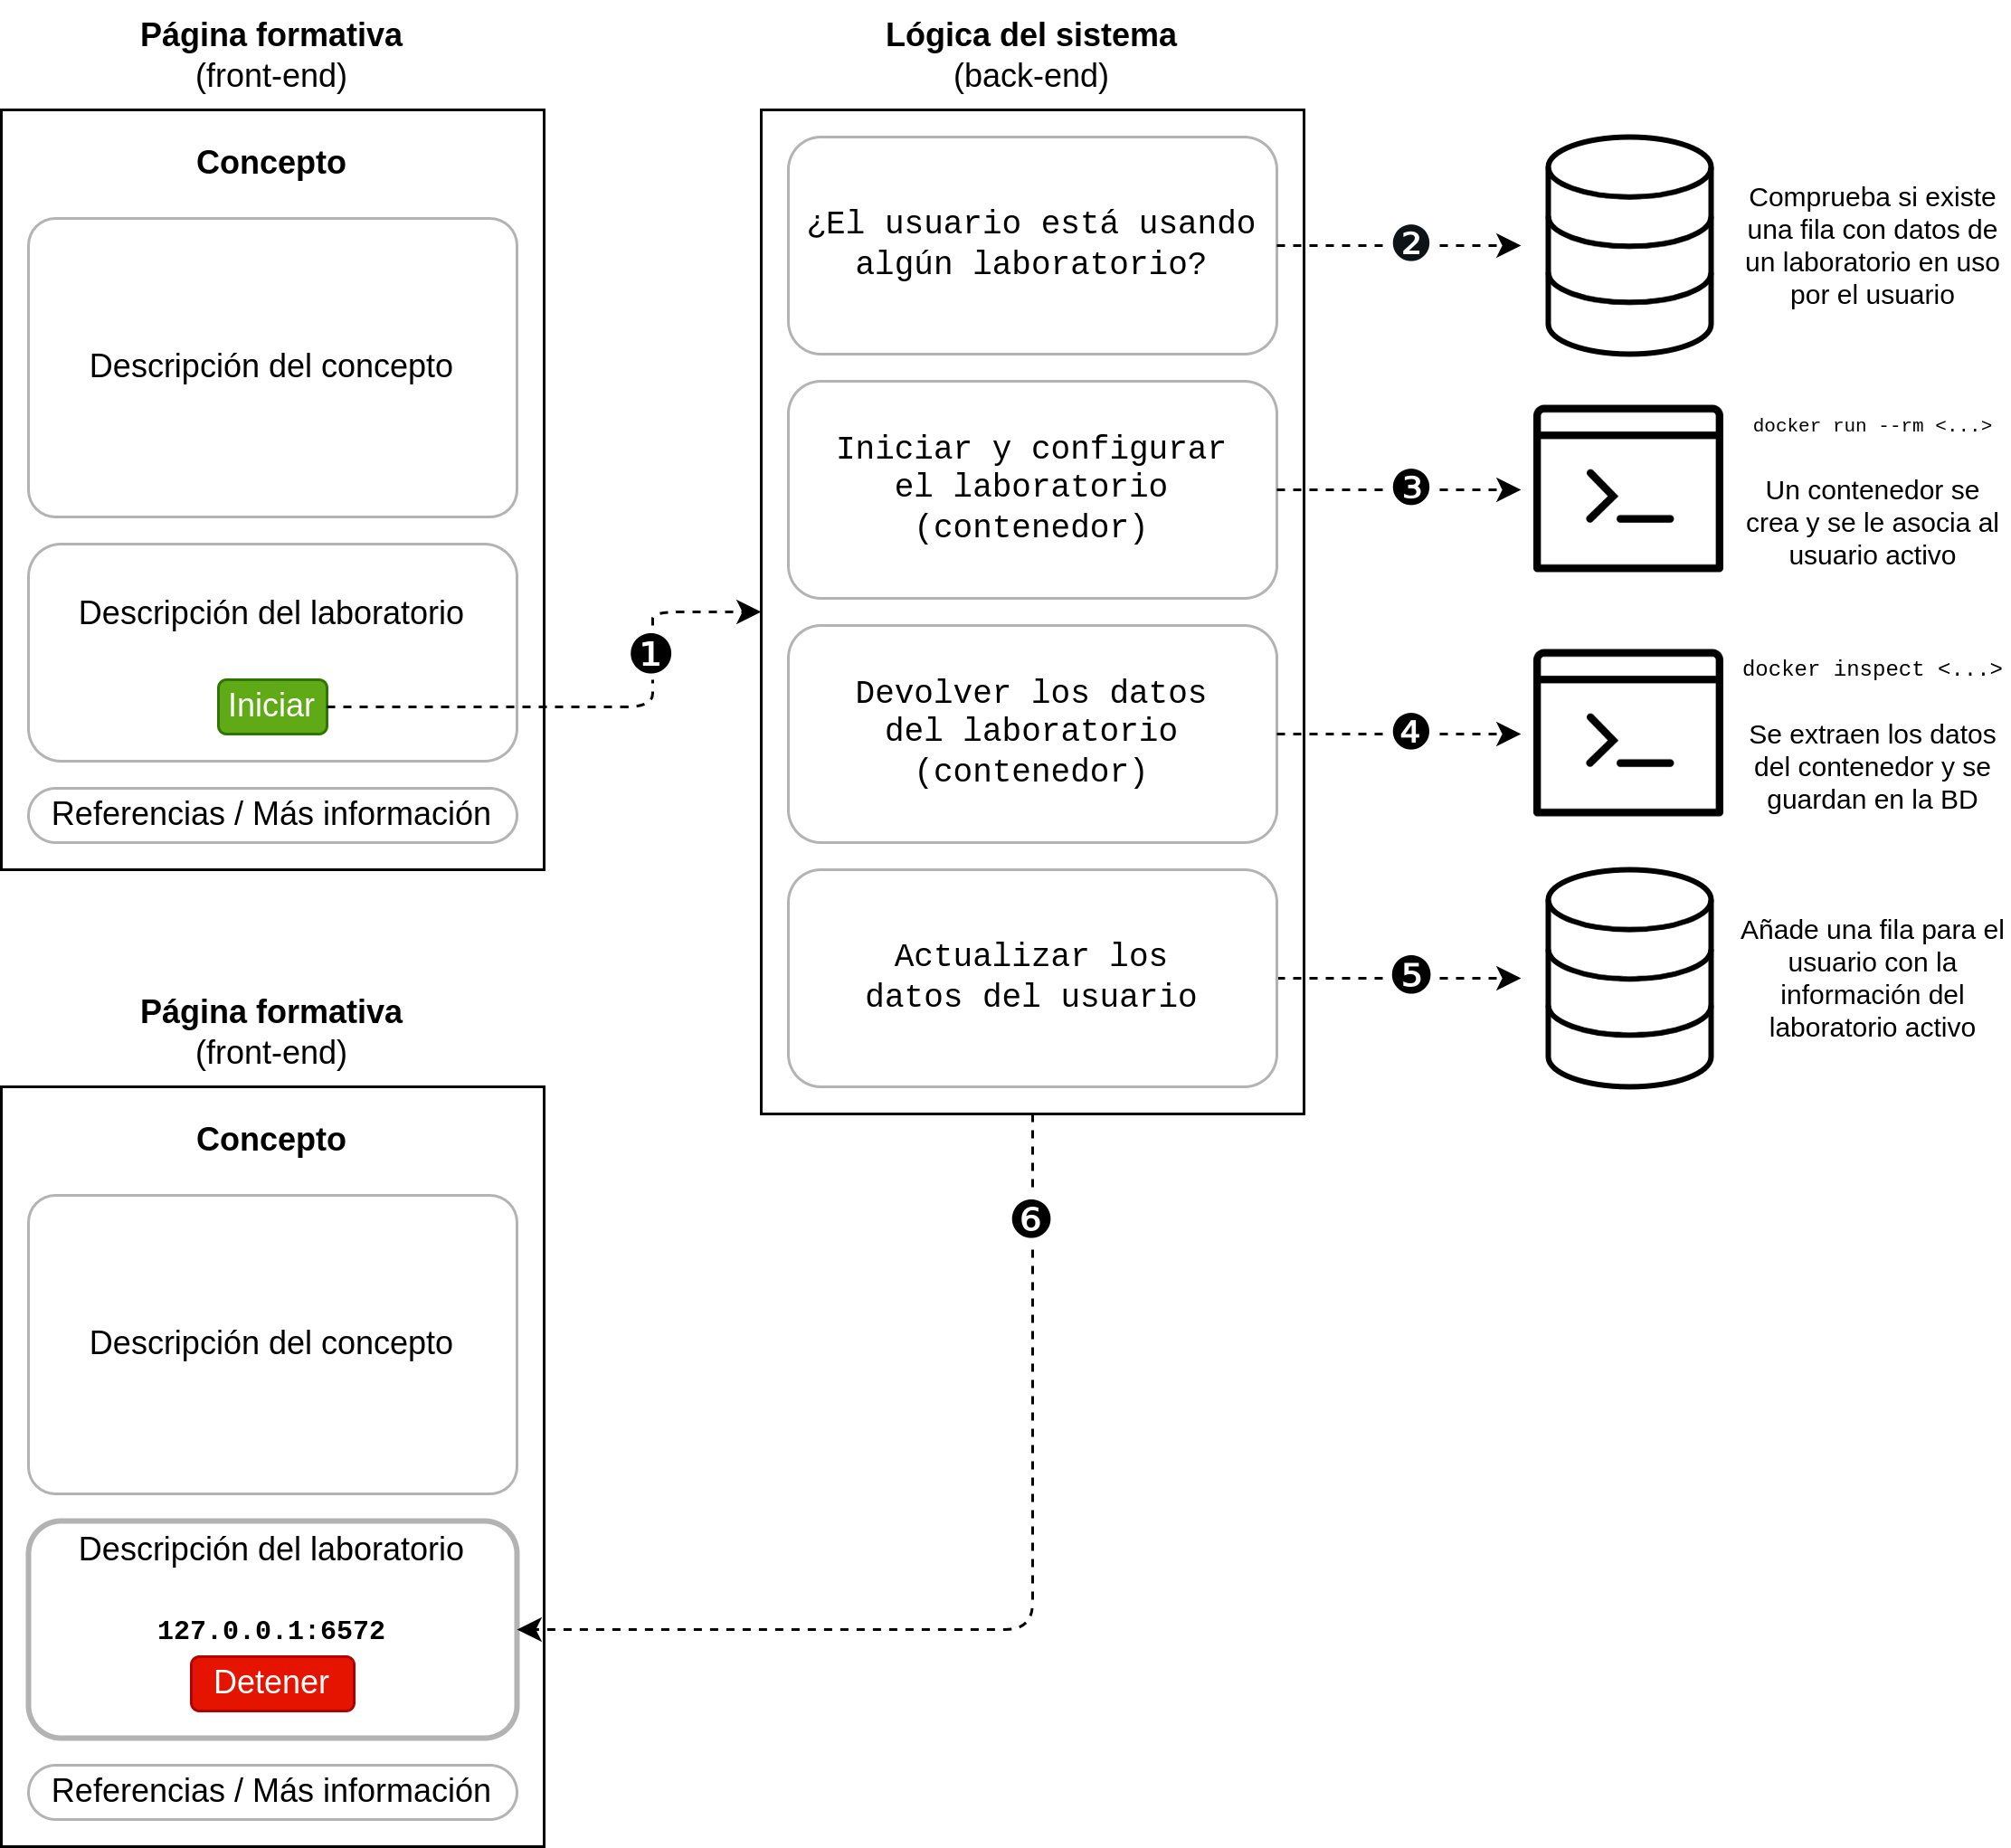
\includegraphics[scale=0.125]{images/Diagramas/iniciar.png}

                \caption{Inicio de un laboratorio desde el sitio web}
                    \label{fig:inicio-laboratorio}
            \end{figure}

            Este diagrama representa un uso normal de la plataforma, donde el usuario accede a la página web y desea iniciar un laboratorio para probar el concepto tratado en la página informativa.

            Se detallan a continuación los pasos que se llevan a cabo:

            \begin{enumerate}
                \item El usuario solicita crear un laboratorio para probar el concepto tratado en la página informativa pulsando el botón de inicio, ejecutando algunas de las funcionalidades de la plataforma definidas en \texttt{functions.php}.

                \item Se comprueba en la base de datos que el usuario activo no tiene ningún otro laboratorio activo. Si lo tuviera, mostraría una advertencia y un enlace a la página del laboratorio activo en la sección \textit{Laboratorio} de la página.

                \item Se obtiene un puerto disponible en el servidor y se hace una llamada al sistema para crear un contenedor Docker mapeando su puerto 22 (SSH por defecto) con el puerto obtenido. La ejecución del comando en el sistema devuelve la ID del contenedor creado, almacenándola en \texttt{functions.php}.

                \item Se vuelve a llamar al sistema para extraer los datos de dicho contenedor usando el ID del paso anterior, porque en el paso anterior el contenedor todavía no existía y por tanto, no era posible extraer información.
                
                \item Se registran los datos recopilados en la base de datos en formato JSON para usar una única celda de la tabla y poder extraerlos cómodamente en \texttt{functions.php}.

                \item Se cambia el estado de la sección \textit{Laboratorio} de la página: se añade la IP de la plataforma (en este caso, \textit{localhost}), el puerto del sistema asociado al contenedor y se cambia el botón de la sección para que ahora detenga el laboratorio.
            \end{enumerate}

            Para facilitar la interpretación, no se han contemplado los errores que pueden ocurrir durante el proceso.
            
            \newpage

            \begin{figure}
                \centering

                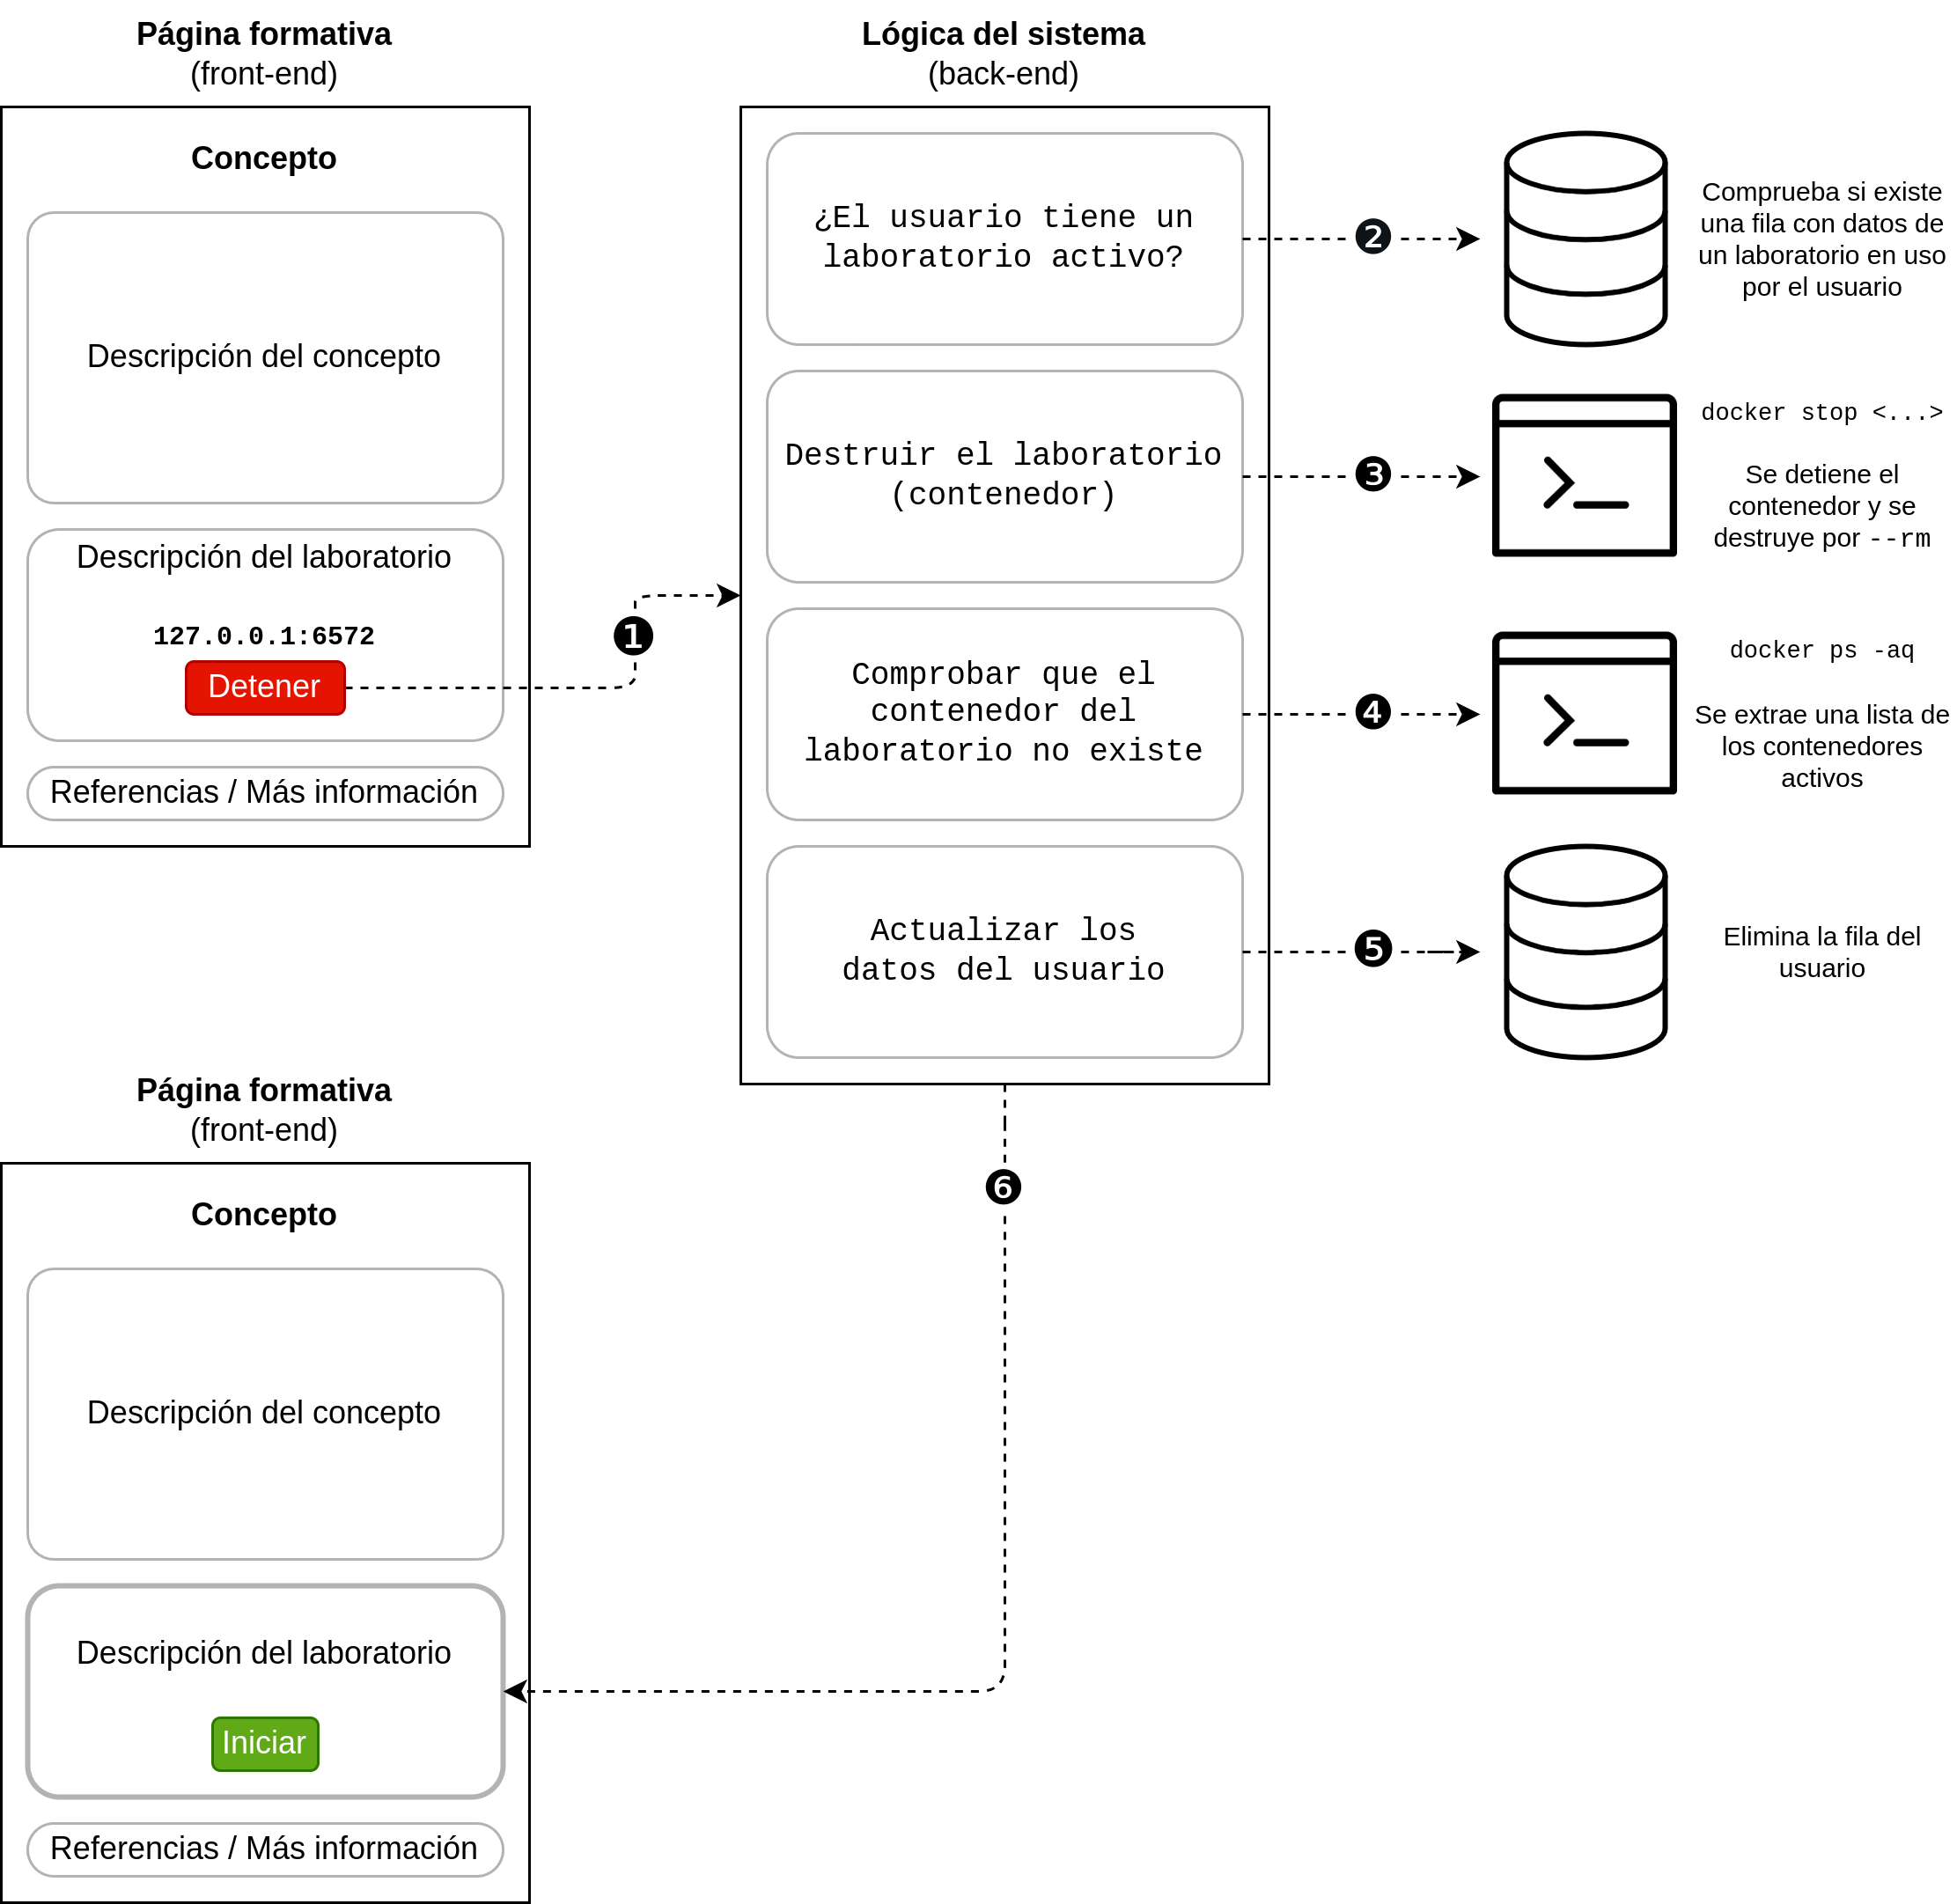
\includegraphics[scale=0.125]{images/Diagramas/detener.png}

                \caption{Destrucción de un laboratorio desde el sitio web}
                    \label{fig:detener-laboratorio}
            \end{figure}

            Este diagrama representa un uso normal de la plataforma, donde el usuario accede a la página web y desea detener el laboratorio activo.

            Se detallan a continuación los pasos que se llevan a cabo:

            \begin{enumerate}
                \item El usuario solicita detener el laboratorio activo porque ha terminado de usarlo (o quiere usar otro) pulsando el botón de detener, ejecutando algunas de las funcionalidades de la plataforma definidas en \texttt{functions.php}.

                \item Se comprueba en la base de datos que el usuario activo tiene un laboratorio activo y se obtienen los datos del mismo.

                \item Se hace una llamada al sistema para detener el contenedor Docker usando la ID obtenida en el paso anterior. Como todos los contenedores se han creado con la opción \texttt{--rm}, al detenerse son eliminados.

                \item Se hace una llamada al sistema para comprobar que el contenedor se ha eliminado correctamente. Se ejecuta el comando \texttt{docker ps -aq} (lista de IDs de todos los contenedores existentes) y se comprueba que no aparece el contenedor en la lista.
                
                \item Se elimina la entrada de la base de datos asociada al laboratorio activo.

                \item Se cambia el estado de la sección \textit{Laboratorio} de la página: se elimina la IP de la plataforma y el puerto del sistema asociado al contenedor y se cambia el botón de la sección para que ahora inicie de nuevo el laboratorio.
            \end{enumerate}

            Para facilitar la interpretación, no se han contemplado los errores que pueden ocurrir durante el proceso.

            \newpage

            \begin{figure}
                \centering

                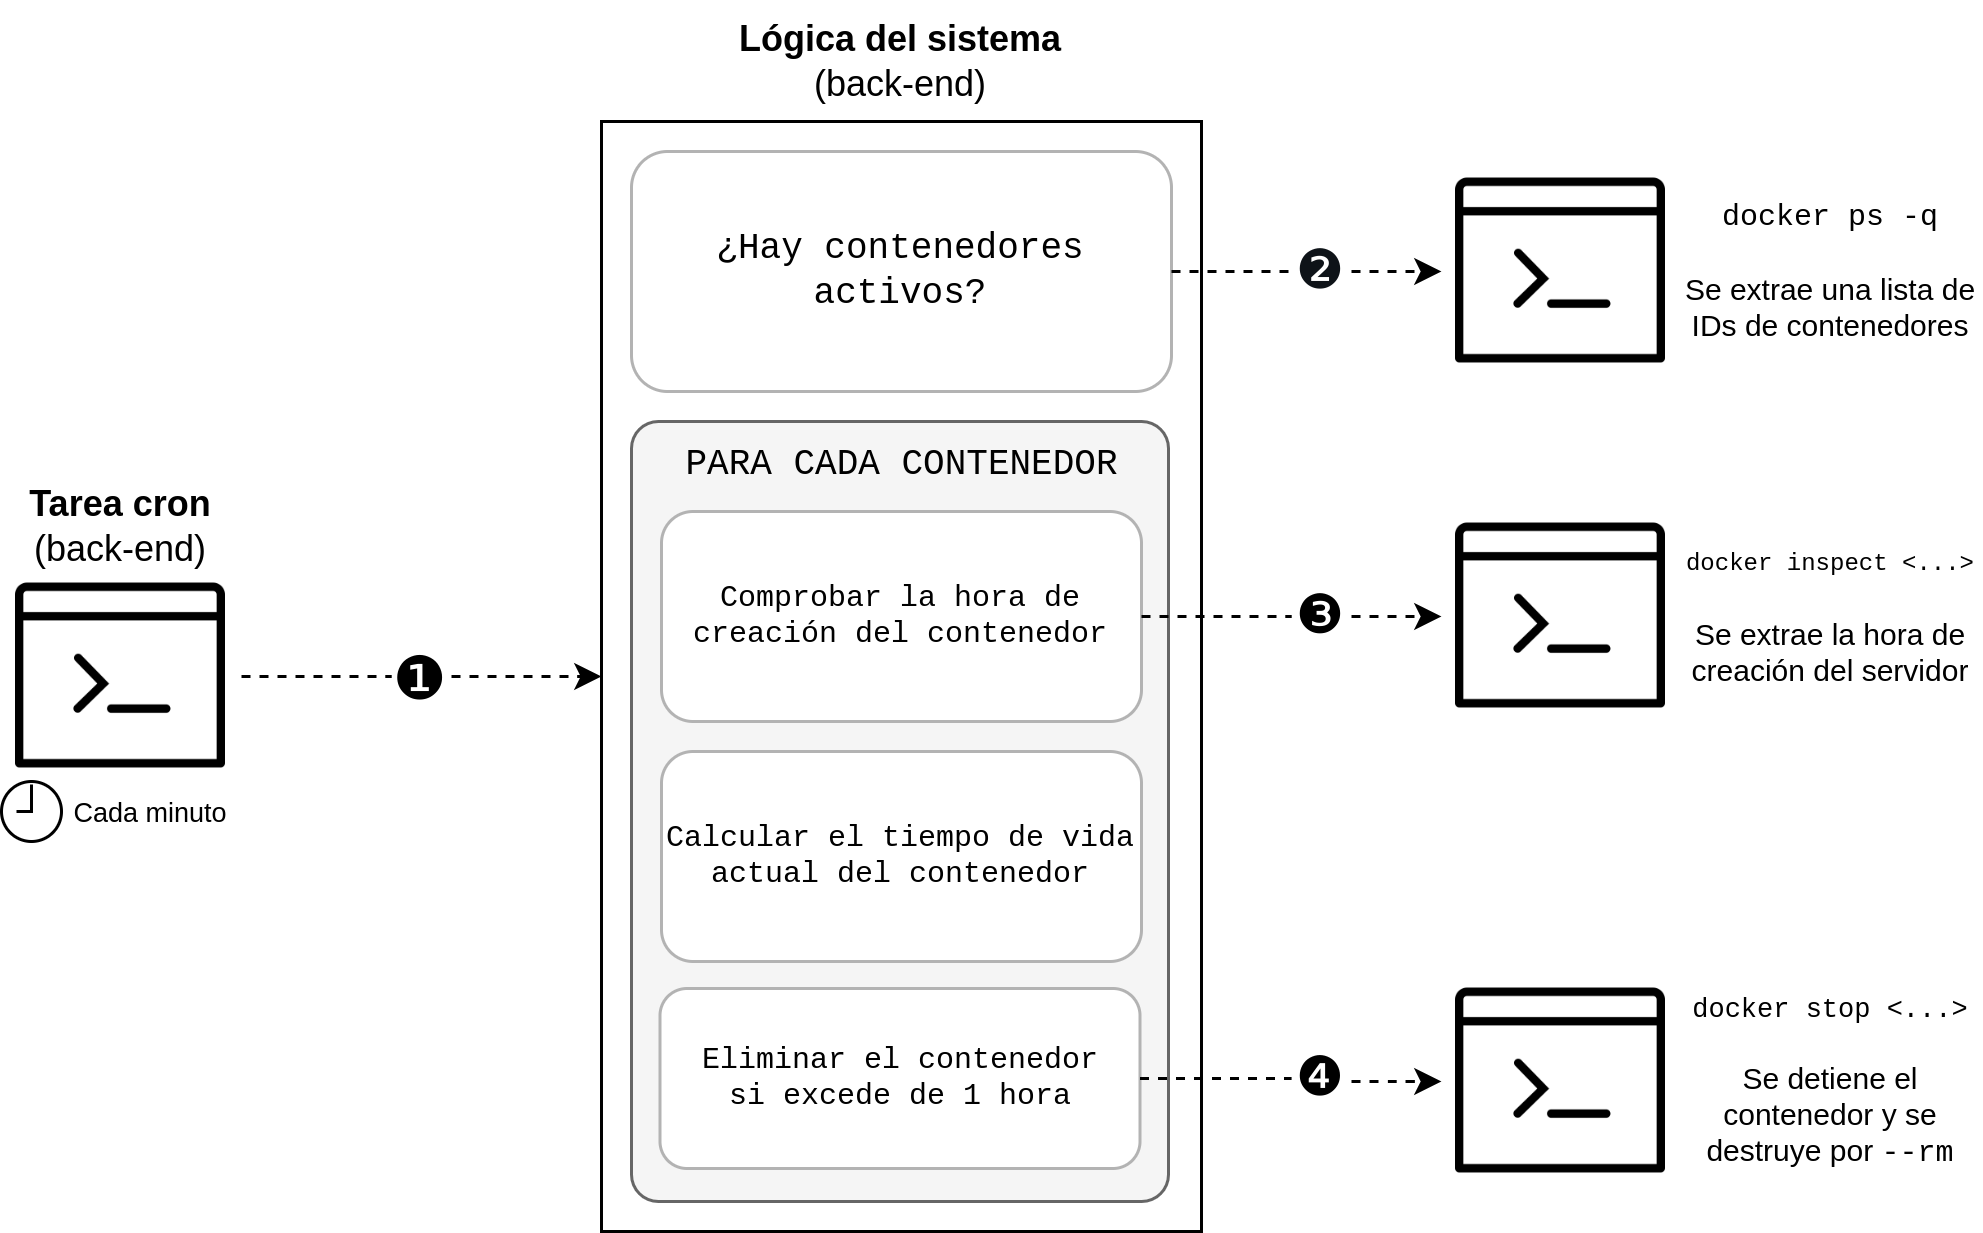
\includegraphics[scale=0.15]{images/Diagramas/detener-cron.png}

                \caption{Destrucción automática de un laboratorio}
                    \label{fig:detener-cron-laboratorio}
            \end{figure}

            Este diagrama representa un uso normal de una tarea de cron con la que detener y eliminar automáticamente laboratorios que excedan su tiempo de vida.

            Se detallan a continuación los pasos que se llevan a cabo:

            \begin{enumerate}
                \item La tarea de cron del sistema ejecuta un script de Bash para detener los contenedores Docker que se encuentren activos y cuyo tiempo de vida exceda a 1 hora. Esta tarea se ejecuta cada minuto.

                \item Se hace una llamada al sistema para comprobar si hay contenedores activos y en caso afirmativo, obtener una lista de los IDs de esos contenedores. El script termina en caso de no haber ninguno.

                \item Se usa la lista en un bucle para iterar sobre ella y se hace una llamada al sistema para obtener la hora de creación del contenedor actual. Esos datos se usan para calcular el tiempo de vida del contenedor actual.
                
                \item Se comprueba si el tiempo de vida del contenedor actual excede a 1 hora y si es así, se detiene. Como los contenedores han sido creados con la opción \texttt{--rm}, al detenerse son eliminados.
            \end{enumerate}

            Este script muestra información cada vez que se ejecuta, haciendo que la tarea de cron almacene dicha información en un archivo de texto a modo de registro.

            \begin{figure}[htbp]
                \centering

                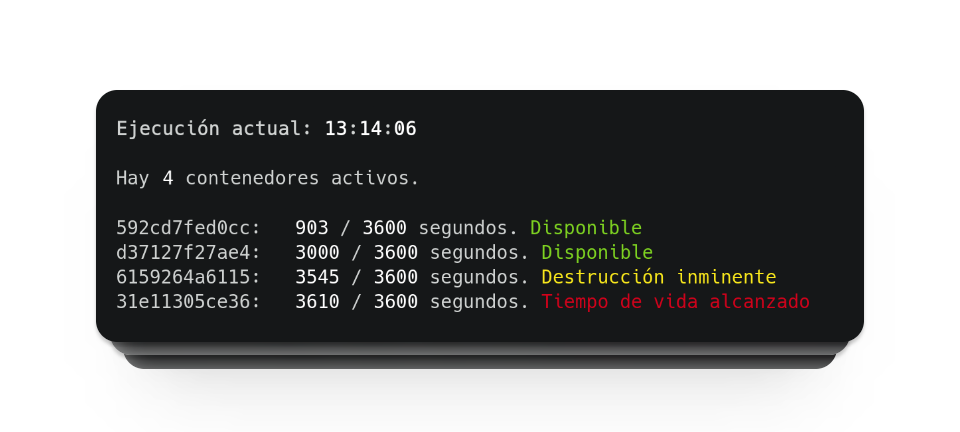
\includegraphics[scale=0.3]{images/Capturas/cron-log.png}

                \caption{Salida del script de la tarea de cron}
                \label{fig:detener-cron-log}
            \end{figure}

            \newpage
        
        
\chapter{Catálogo de conceptos}
    \label{cap:catalogo}

    A continuación se muestra una serie de conceptos relacionados con el pentesting. El catálogo incluye algunos conceptos más genéricos y comunes, así como casos más específicos, todo con el fin de ofrecer al usuario una visión general del pentesting.

    Cada concepto de este capítulo incluye una pequeña descripción, el motivo de su inclusión al sitio web y un resumen de la funcionalidad de su laboratorio asociado.

    Por último, cabe destacar que el texto mostrado en este documento no se corresponde con la versión final -más elaborada y detallada- publicada en el sitio web del proyecto, ya que está orientado a la redacción de este trabajo de fin de grado y no al entorno en producción del usuario final.


    \section{Introducción a Linux}

        Linux es un sistema operativo de código abierto basado en UNIX creado en 1991, y aunque inicialmente fue desarrollado para ordenadores personales, actualmente se utiliza en una gran variedad de dispositivos (servidores, dispositivos móviles, sistemas embebidos, etc.).

        Este concepto se presenta como una introducción al sistema de jerarquía de ficheros y directorios de Linux, así como a la gestión de permisos, grupos y usuarios del sistema. También se incluyó una introducción a la terminal de Linux y a distintos comandos clasificados por categorías.

        \subsection{Motivación}

            Este trabajo de fin de grado está orientado a aquellos usuarios que quieren empezar en el sector del pentesting, por lo que se ha considerado adecuado incluir una breve introducción a Linux, ya que resulta evidente el abundante uso de sistemas operativos basados en UNIX en el sector.

            Tener un profundo conocimiento de la jerarquía de ficheros y directorios, la gestión de permisos, grupos y usuarios, así como el uso de la terminal, es fundamental para llevar a cabo pruebas de penetración efectivas y descubrir posibles vulnerabilidades y puntos débiles en un sistema. Un pentester debe comprender esta jerarquía para ubicar rápidamente recursos críticos y datos sensibles.

            Comprender cómo funcionan los permisos, cómo se asignan a usuarios y grupos específicos, y cómo se heredan en la jerarquía de archivos, es esencial para evaluar la seguridad. Los pentesters pueden identificar vulnerabilidades al explorar archivos con permisos incorrectos, que podrían permitir el acceso no autorizado o la ejecución de comandos peligrosos.

        \subsection{Laboratorio}

            Se proporciona al usuario un entorno virtualizado Linux donde poner en práctica lo mencionado anteriormente, revisar y manipular su contenido, así como ejecutar comandos.

            Este entorno está pensado, principalmente, para aquellos usuarios que no dispongan de un sistema operativo basado en UNIX o que prefieran no modificar el suyo propio para realizar pruebas.

    
    \section{Introducción a Bash}

        Bash (\textit{Bourne Again Shell}) es un lenguaje de scripting que se ejecuta en la terminal de Linux, y que permite automatizar tareas de forma sencilla.

        Este concepto se presenta como una introducción al lenguaje Bash, abarcando desde la sintaxis básica hasta el uso de variables, funciones, bucles y condicionales.

        \subsection{Motivación}

            Bash es un lenguaje de scripting muy popular y ampliamente utilizado en el sector, ya que viene incluido en la mayoría de distribuciones de Linux y es el intérprete de comandos por defecto en la mayoría de ellas.
                        
            Durante una prueba de penetración, hay muchas tareas que se deben realizar de manera repetitiva, como el escaneo de puertos, la recolección de información, la enumeración de servicios, entre otros; es posible crear scripts de Bash que realicen estas tareas automáticamente, lo que ahorra tiempo y reduce errores humanos.

            Resulta común crear exploits o pruebas específicas para aprovechar vulnerabilidades y evaluar la resistencia de un sistema durante una prueba de penetración, por lo que es importante contar con conocimientos de Bash para adaptarse a las necesidades de la prueba y crear scripts personalizados que permitan realizar pruebas de manera eficiente.

            Por último, el proceso de crear scripts en Bash puede fomentar un conocimiento más profundo sobre cómo funcionan los sistemas operativos y las redes, lo que puede mejorar la comprensión general de los conceptos de seguridad informática y permitir al pentester detectar vulnerabilidades que podrían pasar desapercibidas de otra forma.

        \subsection{Laboratorio}

            Se proporciona al usuario un entorno virtualizado Linux donde poner en práctica lo mencionado anteriormente, revisar y manipular su contenido, así como ejecutar comandos.

            Este entorno, al igual que el de \textit{Introducción a Linux}, está pensado para aquellos usuarios que no dispongan de un sistema operativo basado en UNIX o que prefieran no modificar el suyo propio para realizar pruebas.


    \section{Introducción a las redes}

        Una red de ordenadores es un conjunto de dispositivos electrónicos conectados entre sí a través de un medio, que intercambian información y comparten recursos.
            
        Los protocolos de red definen un conjunto de reglas y convenciones para llevar a cabo la comunicación entre dispositivos en una red, incluyendo mecanismos para la autenticación, la transferencia de datos, la detección de errores y la corrección de errores, y la señalización.

        Este concepto se presenta como una introducción a los conceptos básicos de redes, que abarca algunos de los protocolos más comunes, como TCP/IP, UDP y SSH, así como los tipos y topologías de redes, y ataques comunes a redes.

        \subsection{Motivación}

            El conocimiento de las redes ocupa un lugar destacado Entre las habilidades esenciales para llevar a cabo un pentesting efectivo, debido a su importancia fundamental en la seguridad de los sistemas.

            Antes de realizar una prueba de penetración, es vital identificar los objetivos y las áreas de interés en la red, ya que sin esta información, sería difícil determinar qué atacar y dónde centrar los esfuerzos de prueba.

            El conocimiento de las direcciones IP y los protocolos utilizados por los sistemas en la red permite a los profesionales de seguridad seleccionar las herramientas y técnicas adecuadas para las pruebas, porque diferentes sistemas y servicios pueden requerir enfoques de ataque específicos, y esta elección informada es esencial para simular con precisión los métodos utilizados por los atacantes reales.

            Por otra parte, comprender la topología de la red ayuda a identificar puntos débiles, rutas alternativas y posibles vectores de ataque.
        

    \section{Análisis de tráfico}

        Esta es una técnica de ciberseguridad que implica la monitorización y el examen de los datos que fluyen a través de una red de comunicaciones. Puede incluir la recopilación de información sobre el origen y el destino de los datos, el tipo de protocolo utilizado, la cantidad de datos transmitidos y otros metadatos relacionados con el tráfico, etc.

        Este concepto se presenta como una descripción del proceso de análisis de tráfico, que abarca la captura de tráfico de red, el análisis de paquetes y el uso de herramientas de análisis de tráfico, como Wireshark.

        \subsection{Motivación}

            El análisis de tráfico es una habilidad esencial para los profesionales de la seguridad informática, ya que permite identificar y comprender el tráfico de red, lo que facilita la detección de anomalías y de posibles amenazas.

            Durante una prueba de penetración, puede ayudar a identificar sistemas y servicios en la red, así como a comprender cómo interactúan entre sí. Esto permite a los pentesters identificar posibles vulnerabilidades y vectores de ataque, y seleccionar las herramientas y técnicas adecuadas para la prueba.

        \subsection{Laboratorio}

            Este entorno permite al usuario usar Wireshark en el propio navegador, alojando el servicio en otro puerto del servidor, accesible desde la propia plataforma. Contiene 4 capturas de tráfico que involucran los protocolos ICMP, ARP, TCP y FTP.
            
            La página de la plataforma hace un recorrido y explicación de 2 de ellas:

            La captura \texttt{SSL.pcap} contiene el intercambio de datos de una conexión TCP, donde se produce el proceso de \textit{handshake} de SSL/TLS, que permite el cifrado de la conexión. El usuario puede usar Wireshark para explorar distintos detalles sobre las versiones de TLS utilizadas y cómo se han decidido utilizar. Se muestra cómo se han obtenido los algoritmos de cifrados y las características de la conexión.

            La captura \texttt{filezilla.pcap} contiene el intercambio de datos de una conexión FTP, donde se produce el proceso de autenticación del usuario, que permite el acceso al servidor FTP. El usuario puede usar Wireshark para explorar distintos detalles sobre el intercambio de datos, como el usuario y contraseña, así como el uso de comandos FTP para la gestión de archivos. También es posible observar el contenido de los ficheros enviados.

            Las otras 3 capturas, llamadas \texttt{Internet.pcap}, \texttt{ping.pcap} y \texttt{SSH.pcap} muestran información sobre otros protocolos útiles como ICMP, SSH y ARP.


    \section{Introducción al OSINT}
        \label{sec:osint}

        La inteligencia de código abierto (\textit{Open Source INTelligence}) es una técnica de investigación que se basa en la obtención de información a partir de fuentes de acceso público.

        Este concepto se presenta como una introducción a OSINT, abarcando la búsqueda de información en distintas herramientas, como los \textit{Google Dorks}, \textit{Shodan.io}, \textit{VirusTotal} y \textit{WHOIS}.

        \subsection{Motivación}

            Esta técnica se utiliza en el sector de la ciberseguridad para obtener información sobre un objetivo, como puede ser una persona, una empresa o una organización, con el objetivo de realizar un ataque posterior.

        \subsection{Laboratorio}

            Este entorno presenta un proyecto de Python con el que extraer información de una IP de varias fuentes de información, entre las que se encuentran Shodan, VirusTotal y WHOIS.

            El proyecto consiste en una interfaz de línea de comandos que permite al usuario introducir una IP o una lista de IPs (en un archivo de texto) y obtener información de cada una de ellas usando las fuentes mencionadas, entre otras.
            
            \paragraph{Nota} La información de Shodan.io y VirusTotal se obtiene a través de sus APIs públicas, por lo que es necesario tener una cuenta en cada una de ellas y obtener una clave de API para poder usarlas. No usar una clave no afectará al programa más allá de no usar esas 2 fuentes de información.

            La herramienta desarrollada para este laboratorio se explica en mayor profundidad en el apéndice \ref{sec:ip-osint}.
        

    \section{Esteganografía}

        La esteganografía es una técnica de ocultación de información dentro de un archivo, como puede ser una imagen, un vídeo o un archivo de audio, lo que facilita la transmisión de datos confidenciales sin ser detectados.

        Este laboratorio presenta una definición de esteganografía y muestra de herramientas comunes, como \texttt{steghide} y \texttt{exiftools}.

        \subsection{Motivación}

            Esta técnica se utiliza en el sector de la ciberseguridad para ocultar información sensible dentro de archivos que no levanten sospechas, por lo que durante una prueba de penetración, los conocimientos de esteganografía pueden ayudar a descubrir información oculta en archivos multimedia.

        \subsection{Laboratorio}

            Este entorno contiene una serie de imágenes con información oculta en ellas, donde el usuario podrá identificar la información oculta y usar las herramientas mencionadas para extraer dicha información.

            Toda la información oculta está conectada, por lo que es posible llevar a cabo un proceso similar al \textit{footprinting} para obtener una información específica.


    \section{Fuerza bruta}

        La fuerza bruta es una técnica en la que se intenta adivinar una contraseña o credencial de acceso probando diferentes combinaciones hasta encontrar la correcta. Generalmente, usando un diccionario de contraseñas como \textit{rockyou.txt}.

        Este concepto se presenta como una descripción de la técnica de fuerza bruta, abarcando el uso de herramientas para descifrar contraseñas.

        Este apartado es especialmente corto dada la naturaleza básica del concepto, ya que se consideró que no era necesario profundizar en él por su conexión con otros más relevantes, como por ejemplo el hash-cracking (sección \ref{sec:hash-cracking}).

        \subsection{Motivación}

            La fuerza bruta es una técnica muy utilizada en el sector de la ciberseguridad para descifrar contraseñas, ya que es relativamente sencilla de implementar y puede ser muy efectiva si se usa correctamente.

            Este término es la base de muchos otros conceptos y está presente en muchas otras técnicas de penetración, como listado de directorios, enumeración de usuarios, etc.

            Por otra parte, es importante saber identificar y aplicar los diccionarios correctos.

        \subsection{Laboratorio}

            Este entorno presenta un sistema Linux vulnerable, ya que la contraseña del usuario \textit{root} es una contraseña común y pertenece al diccionario \textit{rockyou.txt}.


    \section{Hash-cracking}
        \label{sec:hash-cracking}

        El hash-cracking es una técnica de ataque que se utiliza para obtener la contraseña original a partir de un hash.

        Este concepto se presensta como descripción de la técnica de hash-cracking, abarcando el uso de herramientas para descifrar información.

        \subsection{Motivación}

            Las contraseñas y otros datos sensibles, rara vez se almacenan en texto plano debido a los riesgos de seguridad asociados; en su lugar, se transforman en valores hash utilizando algoritmos de hash criptográficos.
            
            Conocer técnicas de hash-cracking permite a los pentesters evaluar la calidad de las contraseñas utilizadas por los usuarios en un sistema. Si las contraseñas se descifran con relativa facilidad, esto indica que los usuarios están utilizando contraseñas débiles, lo que representa un riesgo de seguridad significativo.
            
            Por último, si los pentesters logran descifrar contraseñas y acceder a cuentas o sistemas protegidos, pueden demostrar el impacto real que tendría un ataque exitoso. Esto es especialmente valioso para concienciar a las partes interesadas sobre la importancia de mejorar la seguridad de las contraseñas y tomar medidas adecuadas.

        \subsection{Laboratorio}

            Este entorno presenta 3 bases de datos cuyas contraseñas han sido almacenadas usando 3 algoritmos de hash diferentes: MD5, SHA1 y SHA256.

            El usuario puede emplear las herramientas descritas en la plataforma para identificar el tipo de hash usado en cada base de datos, y llevar a cabo una extracción de las contraseñas de cada una.

            Además, se le proporciona al usuario una breve guía de comandos SQL para usar, ya que la finalidad de este laboratorio no es el manejo de bases de datos.


    \section{Criptografía}

        La criptografía es una técnica que se utiliza para cifrar y descifrar información, cuyo objetivo es que solo el emisor y el receptor puedan acceder a ella.

        Este concepto se presenta como una introducción a la criptografía, abarcando algunos tipos de cifrado y su clasificación, así como el uso de herramientas de criptografía para cifrar y descifrar mensajes.

        \subsection{Motivación}

            La criptografía está presente en muchos aspectos de la seguridad informática, como la autenticación de usuarios y la firma digital, por lo que es importante conocer los conceptos básicos de la criptografía para comprender cómo funcionan estos mecanismos de seguridad.


    \section{Escalada de privilegios}
    
        La escalada de privilegios es una técnica de hacking que se utiliza para obtener acceso a sistemas o recursos que normalmente estarían restringidos por permisos de seguridad. 

        Este concepto se presenta como una descripción de la técnica de escalada de privilegios y posibles casos de uso de la misma.

        \subsection{Motivación}

            Esta técnica se utiliza cuando un atacante ya ha obtenido acceso a un sistema con un conjunto limitado de permisos, pero necesita obtener permisos adicionales para llevar a cabo acciones malintencionadas, resultando en una habilidad muy útil para la ejecución de pruebas de penetración, ya que si es posible obtener permisos de administrador o de otro usuario privilegiado, el atacante puede tener acceso a información confidencial, instalar malware o tomar el control total del sistema.

        \subsection{Laboratorio}

            Este entorno presenta una vulnerabilidad de permisos débiles; en esta ocasión, el fichero \texttt{/etc/shadow} tiene permisos de lectura para todos los usuarios, por lo que cualquier usuario puede leer el contenido del fichero, que contiene las contraseñas cifradas de los usuarios del sistema.

            Una vez se lee el fichero, se puede observar que existen 2 usuarios: \texttt{root} y \texttt{user}, siendo este último el que maneja la conexión SSH para el usuario de la plataforma.

            Además, haciendo un estudio del formato de los hashes almacenados, es posible llegar a la conclusión de que las contraseñas están usando MD5 crypt, por lo que es posible descifrarlas usando una herramienta de hash-cracking.

            Obteniendo así, la contraseña del usuario \texttt{root} y pudiendo acceder al sistema como administrador.


    \section{Bypass}

        Un bypass es una vulnerabilidad que permite a un atacante evadir un mecanismo de seguridad, como la autenticación, para obtener acceso no autorizado a un sistema o recurso.

        Este concepto se presensta como una descripción del término de bypass, a través de la vulnerabilidad CVE-2017-8386, que permite a un atacante remoto omitir la autenticación en un servidor Git.

        \subsection{Motivación}

            Una vulnerabilidad de bypass puede permitir a un atacante evadir un mecanismo de seguridad, como la autenticación, para obtener acceso no autorizado a un sistema o recurso.

            Esta técnica se utiliza en el sector de la ciberseguridad para obtener acceso a sistemas o recursos que normalmente estarían restringidos por permisos de seguridad, por lo que es importante conocer los conceptos básicos de los bypasses para comprender cómo funcionan estos mecanismos de seguridad y cómo se pueden evitar.

        \subsection{Laboratorio}

            Este laboratorio simula un servidor de Git con la vulnerabilidad CVE-2017-8386.

            Se requiere una clave SSH privada proporcionada en la plataforma para que se realice la conexión correctamente.

            Una vez se hayan completado esos preparativos, se podrá llevar a cabo la explotación mencionada anteriormente y el usuario podrá explorar las posibilidades que ofrece dicho bypass.


    \section{Ransomware}
        \label{sec:ransomware}
        
            Este es un laboratorio especial -algo más alejado del pentesting- que trata la peligrosidad de un ransomware, al mismo tiempo que se observa la sencillez con la que este puede causar mucho daño en un sistema.

        \subsection{Motivación}

            Se ha considerado importante usar una parte de este trabajo de fin de grado para concienciar a los usuarios sobre la amenaza real que supone el ransomware, ya que es una de las amenazas más comunes en la actualidad y puede causar mucho daño en un sistema.

        \subsection{Laboratorio}

            Este entorno contiene una muestra de ransomware muy simple, pero igualmente peligrosa si no se trata con cuidado. El ransomware se llama \texttt{stockholm.py} y ha sido desarrollado en Python.
            
            El script se encuentra en el directorio del usuario \texttt{root} y realizará las siguientes acciones:
            
            \begin{enumerate}
                \item Creará una clave de cifrado aleatoria.
                \item Buscará una carpeta llamada \texttt{infection/} en la carpeta del usuario \texttt{root}.
                \item Usando la clave, cifrará todos los archivos de la carpeta \texttt{infection/} cuya extensión también fuera afectada por \textit{WannaCry}.
                \item Guardará la clave de cifrado de forma segura en un archivo llamado \texttt{clave.key}.
            \end{enumerate}

            No obstante, como solo es una prueba de concepto, el script también puede devolver los archivos a su estado original utilizando la clave de cifrado proporcionada por el mismo (paso 1): ejecutar \texttt{stockholm.py -r \{clave\}} revertirá el cifrado.
            
            El objetivo de este laboratorio es que el usuario observe el funcionamiento de un ransomware y expermiente con él para que pueda entender mejor cómo funcionan y cómo se pueden evitar.

            \cleardoublepage



\chapter{Resultados}

    \section{Cumplimiento de los requisitos}
        
        Se muestran a continuación los requisitos funcionales definidos en el capítulo \ref{sec:ingenieria-requisitos} y su cumplimiento en la plataforma.
        
        Para ello, se ha usado el lenguaje Gherkin \cite{gherkin}, que permite definir requisitos funcionales en un lenguaje natural, y que además, permite definir escenarios de prueba para comprobar el cumplimiento de dichos requisitos.

        \begin{table}[!htbp]
            \centering

            \begin{tabular}{|c|c|}
                \hline
                \textbf{RF - 01} & \textbf{Registro de usuarios} \\
                \hline
                \multicolumn{2}{|p{15cm}|}{
                    El sistema debe permitir que los usuarios se registren y creen una cuenta en la plataforma para poder usar los laboratorios de pruebas.
                } \\                    
                \hline
                \multicolumn{2}{|p{15cm}|}{
                    %% Vacío
                } \\
                \hline
                \textbf{escenario} & \textbf{Registro correcto de un usuario.} \\
                cuando & Estoy en la página de registro. \\
                entonces & Relleno el formulario de registro con datos válidos. \\
                y & Pulso el botón de registro. \\
                entonces & Un mensaje me indica que mi usuario ha sido creado correctamente. \\
                cuando & Estoy en la página de inicio de sesión. \\
                entonces & Puedo iniciar sesión con el usuario que acabo de crear. \\
                \hline
                \multicolumn{2}{|p{15cm}|}{
                    %% Vacío
                } \\
                \hline
                \textbf{escenario} & \textbf{Registro incorrecto de un usuario.} \\
                cuando & Estoy en la página de registro. \\
                entonces & Relleno el formulario de registro con datos inválidos. \\
                y & Pulso el botón de registro. \\
                entonces & Un mensaje me indica que ha ocurrido un error al crear mi usuario. \\
                \hline
            \end{tabular}
        \end{table}

        \begin{table}[!htbp]
            \centering

            \begin{tabular}{|c|c|}
                \hline
                \textbf{RF - 02} & \textbf{Inicio de sesión} \\
                \hline
                \multicolumn{2}{|p{15cm}|}{
                    El sistema debe permitir que los usuarios inicien sesión en la plataforma para poder usar los laboratorios de pruebas.
                } \\                    
                \hline
                \multicolumn{2}{|p{15cm}|}{
                    %% Vacío
                } \\
                \hline
                \textbf{escenario} & \textbf{Inicio de sesión correcto de un usuario.} \\
                cuando & Estoy en la página de inicio de sesión. \\
                entonces & Relleno el formulario de inicio de sesión con datos válidos. \\
                y & Pulso el botón de inicio de sesión. \\
                entonces & Soy redirigido a la página de inicio. \\
                \hline
                \multicolumn{2}{|p{15cm}|}{
                    %% Vacío
                } \\
                \hline
                \textbf{escenario} & \textbf{Inicio de sesión incorrecto de un usuario.} \\
                cuando & Estoy en la página de inicio de sesión. \\
                entonces & Relleno el formulario de inicio de sesión con datos inválidos. \\
                y & Pulso el botón de inicio de sesión. \\
                entonces & Un mensaje me indica que ha ocurrido un error al iniciar sesión. \\
                \hline
            \end{tabular}
        \end{table}

        \begin{table}[!htbp]
            \centering

            \begin{tabular}{|c|c|}
                \hline
                \textbf{RF - 03} & \textbf{Validación de los datos de registro} \\
                \hline
                \multicolumn{2}{|p{15cm}|}{
                    El sistema debe validar los datos de registro de los usuarios para poder crear una cuenta en la plataforma.
                } \\
                \hline
                \multicolumn{2}{|p{15cm}|}{
                    %% Vacío
                } \\
                \hline
                \textbf{escenario} & \textbf{Validación correcta de los datos de registro.} \\
                cuando & Estoy en la página de registro. \\
                entonces & Relleno el formulario de registro con datos válidos. \\
                y & Pulso el botón de registro. \\
                entonces & Un mensaje me indica que mi usuario ha sido creado correctamente. \\
                \hline
                \multicolumn{2}{|p{15cm}|}{
                    %% Vacío
                } \\
                \hline
                \textbf{escenario} & \textbf{Validación incorrecta de los datos de registro.} \\
                cuando & Estoy en la página de registro. \\
                entonces & Relleno el formulario de registro con datos inválidos. \\
                y & Pulso el botón de registro. \\
                entonces & Un mensaje me indica que ha ocurrido un error al crear mi usuario. \\
                \hline
            \end{tabular}
        \end{table}

        \begin{table}[!htbp]
            \centering

            \begin{tabular}{|c|c|}
                \hline
                \textbf{RF - 04} & \textbf{Consulta de documentación} \\
                \hline
                \multicolumn{2}{|p{15cm}|}{
                    El sistema debe permitir que los usuarios consulten la documentación de la plataforma para poder aprender sobre los conceptos de ciberseguridad.
                } \\                    
                \hline
                \multicolumn{2}{|p{15cm}|}{
                    %% Vacío
                } \\
                \hline
                \textbf{escenario} & \textbf{Consulta de documentación.} \\
                cuando & Estoy en la página de laboratorios. \\
                entonces & Puedo ver una lista de conceptos de ciberseguridad. \\
                cuando & Estoy en la página de un concepto. \\
                entonces & Puedo ver una descripción del concepto asociado. \\
                y & Avanzando en la página. \\
                entonces & Puedo ver un laboratorio asociado (si lo hubiera). \\
                \hline
            \end{tabular}
        \end{table}

        \begin{table}[!htbp]
            \centering

            \begin{tabular}{|c|c|}
                \hline
                \textbf{RF - 05} & \textbf{Inicio de laboratorios} \\
                \hline
                \multicolumn{2}{|p{15cm}|}{
                    El sistema debe permitir que los usuarios inicien y detengan laboratorios de pruebas para poder practicar los conceptos de ciberseguridad.
                } \\                    
                \hline
                \multicolumn{2}{|p{15cm}|}{
                    %% Vacío
                } \\
                \hline
                \textbf{escenario} & \textbf{Inicio correcto de un laboratorio de pruebas.} \\
                cuando & Estoy en la página de un concepto. \\
                y & Existe un laboratorio de pruebas asociado. \\
                y & He iniciado sesión en la plataforma. \\
                y & No tengo ningún laboratorio de pruebas activo. \\
                y & Pulso el botón de inicio del laboratorio. \\
                entonces & Se crea un laboratorio de pruebas alojado en un puerto. \\
                \hline
                \textbf{escenario} & \textbf{Inicio incorrecto de un laboratorio de pruebas} \\
                cuando & Estoy en la página de un concepto. \\
                y & Existe un laboratorio de pruebas asociado. \\
                y & No he iniciado sesión en la plataforma. \\
                entonces & Un mensaje me indica que debo iniciar sesión. \\
                cuando & Estoy en la página de un concepto. \\
                y & Existe un laboratorio de pruebas asociado. \\
                y & He iniciado sesión en la plataforma. \\
                y & Tengo un laboratorio de pruebas activo. \\
                entonces & Un mensaje me indica que ya tengo un laboratorio activo. \\
                \hline

            \end{tabular}
        \end{table}

        \begin{table}[!htbp]
            \centering

            \begin{tabular}{|c|c|}
                \hline
                \textbf{RF - 06} & \textbf{Tiempo de vida de un laboratorio} \\
                \hline
                \multicolumn{2}{|p{15cm}|}{
                    El sistema debe permitir que los usuarios inicien y detengan laboratorios de pruebas para poder practicar los conceptos de ciberseguridad.
                } \\
                \hline
                \multicolumn{2}{|p{15cm}|}{
                    %% Vacío
                } \\
                \hline
                \textbf{escenario} & \textbf{Tiempo de vida alcanzado (1 hora).} \\
                cuando & Estoy dentro del laboratorio.\\
                y & El laboratorio alcanza su tiempo de vida. \\
                entonces & El laboratorio se detiene automáticamente. \\
                y & Soy expulsado de la sesión SSH. \\
                \hline
            \end{tabular}
        \end{table}

        \newpage

        \begin{table}[!htbp]
            \centering

            \begin{tabular}{|c|c|}
                \hline
                \textbf{RF - 07} & \textbf{Número máximo de laboratorios} \\
                \hline
                \multicolumn{2}{|p{15cm}|}{
                    El sistema debe permitir que los usuarios inicien y detengan laboratorios de pruebas para poder practicar los conceptos de ciberseguridad.
                } \\
                \hline
                \multicolumn{2}{|p{15cm}|}{
                    %% Vacío
                } \\
                \hline
                \textbf{escenario} & \textbf{Número máximo de laboratorios alcanzado.} \\
                cuando & Estoy en la página de un concepto. \\
                y & Existe un laboratorio de pruebas asociado. \\
                y & He iniciado sesión en la plataforma. \\
                y & Tengo un laboratorio de pruebas activo. \\
                entonces & Un mensaje me indica que ya tengo un laboratorio activo. \\
                \hline
            \end{tabular}
        \end{table}

        \begin{table}[!htbp]
            \centering
            \begin{tabular}{|c|c|}
                \hline
                \textbf{RF - 08} & \textbf{Uso de un laboratorio iniciado} \\
                \hline
                \multicolumn{2}{|p{15cm}|}{
                    El sistema debe permitir que los usuarios inicien y detengan laboratorios de pruebas para poder practicar los conceptos de ciberseguridad.
                } \\
                \hline
                \multicolumn{2}{|p{15cm}|}{
                    %% Vacío
                } \\
                \hline
                \textbf{escenario} & \textbf{Quiero usar un laboratorio que aún no he detenido.} \\
                cuando & Estoy en la página del concepto del laboratorio. \\
                y & Existe un laboratorio de pruebas asociado. \\
                y & He iniciado sesión en la plataforma. \\
                y & Tengo el laboratorio de pruebas activo. \\
                y & El laboratorio no ha alcanzado su tiempo de vida. \\
                entonces & Un mensaje me indica que el laboratorio está activo. \\
                y & Puedo conectarme usando SSH. \\
                \hline
            \end{tabular}
        \end{table}

        \begin{table}[!htbp]
            \centering

            \begin{tabular}{|c|c|}
                \hline
                \textbf{RF - 09} & \textbf{Detener de laboratorios} \\
                \hline
                \multicolumn{2}{|p{15cm}|}{
                    El sistema debe permitir que los usuarios detengan laboratorios de pruebas para poder practicar los conceptos de ciberseguridad.
                } \\                    
                \hline
                \multicolumn{2}{|p{15cm}|}{
                    %% Vacío
                } \\
                \hline
                \textbf{escenario} & \textbf{Detención correcta de un laboratorio de pruebas.} \\
                cuando & Estoy en la página de un concepto. \\
                y & Existe un laboratorio de pruebas asociado. \\
                y & He iniciado sesión en la plataforma. \\
                y & Tengo el laboratorio de pruebas activo. \\
                y & Pulso el botón de detención del laboratorio. \\
                entonces & Se detiene el laboratorio de pruebas alojado en un puerto. \\
                \hline
                \textbf{escenario} & \textbf{Detención incorrecta de un laboratorio de pruebas} \\
                cuando & Estoy en la página de un concepto. \\
                y & Existe un laboratorio de pruebas asociado. \\
                y & No he iniciado sesión en la plataforma. \\
                entonces & Un mensaje me indica que debo iniciar sesión. \\
                \hline
            \end{tabular}
        \end{table}

        \newpage
            
    
    \section{Conclusiones}

        La realización de este proyecto me ha permitido profundizar en el mundo de la ciberseguridad, así como en el desarrollo web y la virtualización con Docker. Considero que me ha servido para ampliar mis conocimientos en estas áreas y para aprender nuevas técnicas y herramientas que no conocía.
    
        Personalmente, tenía 2 objetivos principales al llevar a cabo este proyecto: ampliar mi conocimiento sobre ciberseguridad y pentesting; y aprender sobre Docker.

        Respecto al primer objetivo, he podido adquirir más conocimientos sobre algunos conceptos que ya conocía, como: OSINT, esteganografía y fuerza bruta; pero también he podido avanzar en aquellos otros conceptos en los que considero que era necesario aprender más, como: el análisis de tráfico, la escalada de privilegios y el hash-cracking.
        
        Por otra parte, también me ha resultado útil para revisar algunos conceptos tratados durante la carrera o debido a la misma, como Bash scripting y redes.

        Respecto al segundo objetivo, he aprendido a usar Docker y he sido testigo no solo de la potencia de esta herramienta, sino de la infinidad de posibilidades que esta plantea, tanto en el ámbito de desarrollo, como en el de producción de sistemas y servicios.

        Si bien no ha sido necesario un uso avanzado de Docker para este proyecto, sí he investigado y aprendido acerca de todas sus otras funcionalidades, como los volúmenes, las redes y los ficheros \textit{dockercompose.yml}.

        Por último, con este proyecto también he adquirido experiencia en el desarrollo web a través de una de las herramientas más usadas: WordPress. Nunca trabajé con ella, por lo que considero que ha sido una buena oportunidad para aprender más sobre esta herramienta y cómo funcionan los sitios web construidos sobre ella.

    
    \section{Futuras líneas de trabajo}
        \label{sec:futuras-lineas-trabajo}

        Este proyecto ha consistido en el desarrollo de una plataforma de introducción al pentesting, pero durante el mismo, se han planteado diversas ideas que podrían ser implementadas en un futuro para mejorar la plataforma.

        \subsection{Traslado del proyecto a un servicio de alojamiento}

            Todo el proyecto está alojado en un servidor local, por lo que un siguiente paso natural sería trasladar la plataforma a un servicio de alojamiento, como por ejemplo alguno de los mencionados en la sección \ref{sec:alojamiento}.

            Esto permitiría que la plataforma estuviera disponible públicamente para cualquier usuario con acceso a Internet, facilitando aún más su consumo y su uso.

        \subsection{Expansión del contenido de pentesting}

            Actualmente la plataforma describe 12 conceptos que cubren los aspectos descritos en la sección \ref{cap:catalogo}, pero se podrían describir y añadir más conceptos junto a sus laboratorios, para ampliar el contenido de la plataforma y ofrecer más experiencias instructivas a los usuarios.

            Por ejemplo: simulación de nuevos ataques, explotación de vulnerabilidades, etc.
        
        \subsection{Optimización de la plataforma}

            La plataforma está construida sobre WordPress, pero se podría plantear la posibilidad de desarrollarla desde cero, ya que WordPress es una herramienta muy potente, pero también muy pesada, por lo que podría ser interesante desarrollar una plataforma más ligera y personalizada.

            Por otra parte, también existen herramientas alternativas que han sido diseñadas específicamente para crear plataformas de CTFs, como: Mellivora \cite{mellivora}, CTFd \cite{ctfd}, Root The Box \cite{root-the-box}, etc.

            \paragraph{Importante}
            
                Cabe destacar que \textbf{este proyecto no es una plataforma de CTFs}, ni debe serlo, ya que los laboratorios planteados quedan a disposición completa del usuario para que los use como desee. Sin embargo, sí podría ser interesante investigar estas herramientas y quizás, aplicar modificaciones para que las pruebas virtualizadas no requieran de una bandera, convirtiendo la plataforma en una herramienta de aprendizaje y no de competición.
            
        \subsection{Generalización del contenido}
            
            El contenido inicial de la plataforma está enfocado al pentesting, pero podría establecerse una temática genérica para abarcar muchos más conceptos de distintas áreas de la seguridad.
            
            Por ejemplo: administración de sistemas, análisis de malware, desarrollo seguro, hacking web, etc. diferentes ramas y especializaciones de ciberseguridad.
            
            Esto daría lugar a una plataforma más eficiente y parecida a otras ya existentes, pero manteniendo la diferencia que se fomentaba al inicio del proyecto en la sección \ref{sec:objetivos}: una plataforma ligera, \textit{open-source} y fácilmente extensible, que permita a los usuarios aprender y practicar conceptos de ciberseguridad mediante laboratorios.

        \subsection{Organización de contenido}
        
            Elaboración de \textit{módulos} o \textit{rutas} de aprendizaje que permitan al usuario seguir un orden lógico al adquirir conocimientos, en lugar de elegir un conceptos al azar o tratar de asumir un orden por su cuenta.

            Por ejemplo: un módulo de introducción a redes, otro de ciber-defensa, etc; una ruta para aprender sobre herramientas de fuerza bruta y explorar sus posibilidades, otra para herramientas como IDS o IPS, etc.

            Esto podría favorecer a la velocidad de aprendizaje del usuario, ya que no tendría que pensar en qué concepto aprender a continuación, sino que podría seguir una ruta de aprendizaje establecida por la plataforma, diseñada para que las conexiones entre las temáticas sean más claras y lógicas.

            \cleardoublepage
